\documentclass[conference,a4paper]{IEEEtran}

\usepackage[noadjust]{cite}
\usepackage[utf8]{inputenc}
\usepackage{csquotes}
\usepackage{textcomp}
\usepackage{pifont}
\usepackage{hyperref}
\usepackage{amsmath}
\usepackage{makecell}
\usepackage{xcolor}
\usepackage{multirow}
\usepackage{booktabs}
\usepackage{graphicx}
\usepackage{subcaption}
\usepackage{amssymb}


\usepackage{tabularx}
\def\tabularxcolumn#1{m{#1}} % vertical centering in tabularx cells
\newcolumntype{Y}{>{\centering\arraybackslash}X} % cell type Y for centered text with automatic line breaks
\newcommand*\rot{\rotatebox{90}} % rotates content 90deg ccw, mainly for table headers
\newcommand*\OK{\ding{51}} % a checkmark-style sign




\bibliography{literature.bib}

\title{A Comparison of Graph Processing Systems}

\author{\IEEEauthorblockN{Simon König}
\IEEEauthorblockA{(3344789)\\
st156571@stud.uni-stuttgart.de}
\and
\IEEEauthorblockN{Leon Matzner}
\IEEEauthorblockA{(3315161)\\
st155698@stud.uni-stuttgart.de}
\and
\IEEEauthorblockN{Felix Rollbühler}
\IEEEauthorblockA{(3310069)\\
st154960@stud.uni-stuttgart.de}
\and
\IEEEauthorblockN{Jakob Schmid}
\IEEEauthorblockA{(3341630)\\
st157100@stud.uni-stuttgart.de}}

\date{\today}



\begin{document}

\maketitle


\begin{abstract}
TODO
\end{abstract}

\begin{IEEEkeywords}
graphs, distributed computing, Galois, Ligra, Polymer, Giraph, Gluon, Gemini
\end{IEEEkeywords}



\section{Introduction}
In recent years graph sizes have increased significantly [?] .
Thus performance and memory efficiency of the graph analysis applications is now more important than ever. 

Many applications like 

Wachsende graphen,
benötigt für folgende Applikationen,
verwenden graph algorithmen,
diese müssen schnell und verteilt laufen
dafür wurden Frameworks entwickelt...

und das noch schön formulieren


We compare several non-uniform memory access (NUMA) aware systems in terms of their performance on three graph algorithms (PageRank, SSSP, BFS).
The comparison is performed on both real world data sets and synthetic graphs. 

To provide a comparison to a non-NUMA aware system, Giraph\cite{Giraph} is included in the testing. Giraph itself has often been compared to other state of the art systems like Pregel or GraphX.



%One of the most famous is the (closed source) distributed graph processing system Pregel. Pregel and several open source versions of .
%This results in suboptimal performance, due to missing cache locality, because the Pregel like systems are written in an object oriented manner relying on pointer chasing mechanisms. 


To this end several non-uniform memory access (NUMA) aware systems were proposed like Polymer \cite{Polymer}, Galois \cite{Galois} or Ligra \cite{Ligra}.



This paper makes the following contributions:
\begin{itemize}
  \item Comparison of several state-of-the-art graph processing frameworks
  \item
  \item
  \item
\end{itemize}

\section{Preliminaries}

\paragraph{Graphs and Paths}
An \emph{unweighted graph} is the pair $G=(V,E)$ where the \emph{vertex set} is $V\subseteq\mathbb N$ and the $E$ is the \emph{edge set}.
The edge set describes a number of connections or relations between two vertices. Depending on these relations, a graph can be directed or undirected. For a \emph{directed graph} the edge set becomes 
\begin{equation*}
  E\subseteq\{(x,y)\,|\, x,y\in V, x\neq y\}
\end{equation*}
and in the \emph{undirected} case $E$ is a set of two-sets 
\begin{equation*}
  E\subseteq\{\{x,y\}\,|\, x,y\in V, x\neq y\}.
\end{equation*}

The main difference is thus, that in the case of a directed graph a connection between $s$ and $t$ is not the same as a connection between $t$ and $s$ -- the direction matters.

Independently of the graph being directed or not, a graph can be \emph{weighted}. In this case the edge set is expanded by a numerical value $E_{\text{weighted}}=E_{\text{unweighted}}\times \mathbb R$ further describing the relation.

The size of a graph is often described in the number of edges $|E|$ because this number is typically much larger than the number of vertices $|V|$.

A \emph{Path} from start $s$ to target $t$ is a set of edges $P\subseteq E^n$ with
\begin{equation*}
   P=((x_0,x_1),(x_1,x_2),\ldots, (x_{n-1},x_n))
\end{equation*}
where all $(x_i,x_{i+1})\in E$ and $x_0=s, x_n=t$.

Thus we call a target $t$ \emph{accessible} from $s$ if a Path from $s$ to $t$ exists.

\paragraph{Single-Source Shortest-Paths}
Single-Source Shortest-Paths (SSSP) describes the problem of finding a path along some edges of the input graph from a given start node to a target.

Input to the problem is a weighted graph $G=(V,E)$ and a start node $s\in V$. Output is the shortest possible distance from $s$ to each node in $V$. 
The distance is defined as the sum of edge weights $w_i$ on a path from $s$ to the target.
In the case of a unweighted graph, the distance is often described in \emph{hops}, i.e. the number of edges on a path.

The most common implementations are Dijkstra's algorithm or BellmanFord.

\paragraph{Breadth-First Search}
Breadth-first search (BFS) is a search problem on a graph. It usually requires an unweighted graph and a start vertex as input. In some cases a target vertex is also given.

The output is usually a set of vertices that are accessible from the start vertex. In the case of a target being given, the output is true if a path from start to target exists or false otherwise.

\paragraph{PageRank}



\paragraph{Pregel Model}




% Google, to overcome, these challenges came up with Pregel.
% Provides scalability
% Fault-tolerance
% Flexibility to express arbitrary algorithms
% The high level organization of Pregel programs
% is inspired by Valiant’s Bulk Synchronous
%  Parallel model 
\paragraph{Congest Model}


\section{Overview of the framworks}
\subsection{Galois and Gluon}
%!TEX root=main.tex

Galois \cite{Galois} is a general purpose library designed for parallel programming. The Galois system supports fine grain tasks, allows for autonomous, speculative execution of these tasks and grants control over the task scheduling policies to the application. It also simplifies the implementation of parallel applications by providing an implicitly parallel unordered-set iterator.\\
For graph analytics purposes a topology aware work stealing scheduler, a priority scheduler and a library of scalable data structures have been implemented. Galois includes applications for for many graph analytics problems, among these are single-source shorthest-paths (sssp) and pagerank. Both of these applications can be executed in shared memory systems and due to the Gluon integration in a distributed environment.\\
Gluon \cite{vertGalois} reduces the communication overhead needed in distributed systems for graph analysis by exploiting structural and temporal invariants.


\subsection{Gemini}
%!TEX root=../../main.tex



\subsection{Giraph}
%!TEX root=../../main.tex
Apache Giraph is an example for an open-source system similar to Pregel.
Thus, Giraph's computation model is closely related to the BSP model discussed in \autoref{sec:bsp}. 
This means that Giraph is based on computation units that communicate using messages and are synchonized with barriers \cite{Giraph}.

The input to a Giraph computation is always a directed graph. Not only the edges but also the vertices have a value attached to them. The graph topology is thus not only defined by the vertices and edges but also their initial values.
Furthermore, one can mutate the graph by adding or removing vertices and edges during computation.

The computation is vertex oriented and iterative.
For each iteration step called superstep, the \emph{compute} method implementing the algorithm is invoked on each active vertex, with every vertex being active in the beginning.
This method receives messages sent in the previous superstep as well as its vertex value and the values of outgoing edges.
With this data, the vertex values are modified and messages to other vertices are sent.
Communication between vertices is only performed via messages, so a vertex has no direct access to values of other vertices. The only visible information is the set of attached edges and their weights.
Supersteps are synchronized using barriers, meaning that all messages only get delivered in the following superstep and computation for the next superstep can only begin after every vertex has finished computing the current superstep.
Edge and vertex values are retained across supersteps.
Any vertex can stop computing (i.e. setting its state to inactive) at any time but incoming messages will reactivate the vertex.
A vote-to-halt method is applied, i.e. if all vertices are inactive or if a user defined superstep number is reached the computation ends.
Once calculation is finished, each vertex outputs some local information (e.g. the final vertex value) as result.

In order for Giraph to achieve scalability and parallelization, it is built on top of Apache Hadoop \cite{Giraph}.
Hadoop is a MapReduce infrastructure providing a fault tolerant basis for large scale data processing.
Hadoop supplies a distributed file system (HDFS), on which all computations are performed.
Giraph is thus, even when only using a single node, running in a distributed manner.
Hence, expanding single-node processing to a multi-node cluster is seamless.
Giraph uses the Map functionality of Hadoop to run the algorithms. Reduce is only used as the identity function.

Giraph being an Apache project makes it the most actively maintained and tested project in our comparison. While writing this paper, several new updates were pushed to Giraph's source repository\footnote{\url{https://gitbox.apache.org/repos/asf?p=giraph.git}}.


\subsection{Ligra}
%!TEX root=../../main.tex

Ligra is a lightweight graph processing framework for shared memory machines \cite{Ligra}. It offers a vertex-centric programming interface which can be used to apply a function to each vertex or outgoing edge of a set of vertices in parallel. While doing so the framework can generate a set of active vertices for the next iteration. This abstraction makes it well suited for writing graph traversal algorithms.

When mapping over edges Ligra optimizes algorithms by switching between a push-based and a pull-based approach based on the size of the set. When the size of the set is above a threshold a pull approach is used. If the threshold is not reached a push approach is used.


\subsection{Polymer}
%!TEX root=main.tex

\subsection{Polymer}
Installing Polymer is straight forward.




\section{And}
%!TEX root = ../main.tex

\subsection{An Overview of Important Graph Formats}
Since every frameworks uses different graph input formats, we supply a conversion tool capable of translating from EdgeList to the required formats.
Data Sets retreived from KONECT can be directly read and translated.

The following sections explain the output formats of our conversion tool.
\subsubsection{AdjacencyList}
The AdjacencyList and WeightedAdjacencyList formats are used by Ligra and Polymer. The format was initially specified for the Problem Based Benchmark Suite, an open source repository to compare different parallel programming methodologies in terms of performance and code quality \cite{pbbs}.

The file looks as follows
\begin{equation*}
	n, m, o_1, \ldots, o_n, t_1, \ldots, t_m
\end{equation*}
where commas are \texttt{\textbackslash n}. First, $n$ is the number of vertices and $m$ the number of edges in the graph.

The $o_k$ are the so-called offsets. Each vertex $k$ has an offset $o_k$, that describes an index in the following list of the $t_i$.
The $t_i$ are vertex IDs describing target nodes of a directed edge. 
The index $o_k$ in the list of target nodes is the point where edges outgoing from vertex $k$ begin to be declared. So vertex $k$ has the outgoing edges
\begin{equation*}
	(k, t_{o_k}), (k, t_{o_k+1}),\ldots, (k, t_{o_{k+1}-1}).
\end{equation*}

For the WeightedAdjacencyList format, the weights are appended to the end of the file in an order corresponding to the target nodes.

\subsubsection{EdgeList}
The EdgeList format is the most intuitive and one of the most commonly used in online data set repositories. The KONECT database uses this format and thus it is the input format for our conversion tool.

An edge list is a set of directed eges $(s_1,t_1),(s_2,t_2),\ldots$ where $s_i$ is a vertex ID representing the start vertex and $t_i$ is a vertex ID representing the target vertex.
In the format, there is one edges per line and the vertex IDs $s_i, t_i$ are separated with any whitespace character.

For a WeightedEdgeList, the edge weights are appended to each line, again separated by a whitespace character.

\subsubsection{Binary EdgeList}
The binary EdgeList format is used by Gemini.

For $s_i, t_i$ some vertex IDs and $w_i$ the weight of a directed edge $(s_i,t_i, w_i)$, Gemini requires the following input format
\begin{equation*}
	s_1t_1w_1s_2t_2w_2\ldots
\end{equation*}
where $s_i,t_i$ have \texttt{uint32} data type and the optional weights are \texttt{float32}.
Gemini will derive the number of edges from the file size, so there is no file header or anything similar allowed.

\subsubsection{Giraph's I/O formats}
Giraph is capable of parsing many different input and output formats. All of those are explained in Giraph's JavaDoc\footnote{\url{http://giraph.apache.org/apidocs/index.html}}.
Both edge- and vertex-centric input formats are possible.

One can even define their own input graph representation or output format. For the purposes of this paper, we used an existing format similar to AdjacencyList but represented in a JSON-like manner.

In this format, the vertex IDs are specified as \texttt{long} with \texttt{double} vertex values, \texttt{float} out-edge weights.
Each line in the graph file looks as follows
\begin{equation*}
	[s,v_s,[[t_1, w_{t_1}], [t_2, w_{t_2}]...]]
\end{equation*}
with $s$ being a vertex ID, $v_s$ the vertex value of vertex $s$. The values $t_i$ are vertices for which an edge from $s$ to $t_i$ exists. The directed edge $(s,t_i)$ has weight $w_{t_i}$.

There is no surrounding pair of brackets and no commas separating the lines as it would be expected in a JSON format.
%hier oder supplementary data?

\section{Testing methods}
%!TEX root=../main.tex


\subsection{Testing Methods}
The testing methods cover the test environment, including hardware and the setup of the frameworks, the graphs used, followed by the algorithms utilized and how the times are measured. 

\subsubsection{Environment}
For testing the graph processing systems, we used 5 machines with two AMD EPYC 7401 (24-Cores) and 256 GB of RAM each. One of those machines was only used as part of the distributed cluster, since it only has 128 GB of RAM.
All five machines were running Ubuntu 18.04.2 LTS.

The setup of each framework was performed according to our provided installation guides available in Appendix \ref{app:installationGuides}.
All benchmark cases were initiated by our benchmark script available in our repository.
All five frameworks are tested on a single server.
Galois, Gemini and Giraph were benchmarked in on the distributed 5-node cluster as well.
Since Galois supports this parameter, we ran multiple tests comparing Galois' performance with different thread counts on a single machine.
Furthermore, Galois is a framework capable of utilizing hugepages. We include an evaluation using those on the single node as well.
Unless mentioned otherwise, we always show results of each framework utilizing 96 threads (i.e. the maximum on our machines) for the single-node evaluation.
The complete benchmark log files and extracted raw results are available in our repository\footnote{\url{https://github.com/SerenGTI/Forschungsprojekt}}.


\subsubsection{Data Sets}
The graphs used in our testing can be seen in detail in \autoref{tbl:graphs}. We included a variaty of different graph sizes, from relatively small graphs like the flickr graph with 2 million edges up to an rMat28 with 4.2 billion edges. All graphs except the rMat27 and rMat28 are exemplary real-world graphs and were retrieved from the graph database\footnote{\url{http://konect.uni-koblenz.de/}} associated with the Koblenz Network Collection (KONECT)\cite{konect}.
Both the rMat27 and rMat28 were created with a modified version of a graph generator provided by Ligra (we changed the output format to EdgeList).
\begin{table}
	\centering
	\caption{Size Comparison of the Used Graphs}
	\begin{tabular}{crr}
		\hline
		\bf{Graph}&\# Vertices (M)&\# Edges (M)\\\hline
		flickr&    		0.1&  2\\
		orkut&          3&    117\\
		wikipedia&      12&   378\\
		twitter&     	52&   1963\\
		rMat27&         63&   2147\\
		friendster&     68&   2586\\
		rMat28&         121&  4294\\
		\hline
	\end{tabular}
	\label{tbl:graphs}
\end{table}

\subsubsection{Algorithms}
The three problems Breadth-first search (BFS), PageRank (PR) and Single-source shortest-path (SSSP) were used to benchmark each framework with every graph.
We always show the results of PageRank with a maximum of five iterations.
For frameworks that support multiple implementations (i.e. PageRank in push and pull modes), we included both in our evaluation.
We chose SSSP and BFS because they are iterative traversal algorithms. Active vertices typically are locally concentrated in the graph. The results of these algorithms can give some insight on the behaviour of the framework with other, similar behaving algorithms.
PageRank on the other hand is an algorithm that is very different to SSSP or BFS for that matter. With PR, there are many active vertices spread across the entire graph, enforcing different data handling strategies from the framework.

In detail, the algorithms for each framework are:
\todo{Algorithmen auflisten}
\begin{itemize}
	\item Ligra supports SSSP based on BellmanFord, BFS and two implementations of PageRank. The two implementations are a regular PR and a Delata Variant.
	\item Polymer supports the same algoritms as ligra.
	\item Gemini supports all of our tested algorithms and there are no setting options or specifications which implementations for the algorithms are used.
	\item Galois supports all of our tested algorithms too, with both a Push and a Pull variant for PageRank available. In the distributed scenario, there are Push and Pull versions for SSSP and BFS available as well. It also supports multiple implementations of the shared-memory allgorithms. The default implementation of SSSP is deltaTile. A lot of setting options are avilable as well, but we're gone with the defaults.
	\item Giraph does not natively supply a BFS algorithm, so in our comparisons a custom implementation is used. For SSSP, slight variations had to be made to the default implementation, to allow us to use different start vertices. For PageRank the supplied implementation is used.
\end{itemize}


\subsubsection{Measurements}
For every framework, we measured the \emph{execution time} as the time from start to finish of the console command.
For the \emph{calculation time}, we tried to extract only the time the framework actually executed the algorithm.
Furthermore, the \emph{overhead} is the time difference between execution time and calculation time. This includes time to read the input graph, initialization and any other tasks other than the actual user-defined algorithm.
Measuring the execution time is straight forward and was done using console time stamps.
For measuring the calculation time, we came up with the following:
\begin{itemize}
	\item For Galois, we extract console log time stamps. Galois outputs \enquote{\texttt{Reading graph complete.}}. Calculation time is the time from this output to the end of execution.

	This is not the most realiable way for measuring the calculation times.
	Not only due to unavoidable buffering in the console output we expect the measured time to be larger than the actual.
	First, it is not clear that all initialization is in fact complete after reading the graph. Second, we include time in the measurement that is used for cleanup after calculation.

	However, this method is the only way of retreiving any measurements without introducing custom modifications to the Galois source code.

	\item Polymer outputs the name of the algorithm followed by an internally measured time.

	\item Gemini outputs a line \texttt{exec\_time=x}, which was used to measure the calculation time.

	\item Ligra outputs its time measurement with \texttt{Running time : x}.

	\item Giraph has built in timers for the iterations (supersteps), the sum of those is the computation time.
\end{itemize}
Each evaluation consisting of graph, framework and algorithm was run 10 times, allowing us to smooth slight variations in the measured times.
Later on, we provide the mean values of the individual times as well as the standard deviation where meaningful.


\section{Results}
%!TEX root=../../main.tex

\subsection{Results}
Ahead of the discussion of the results a few of the issues we encountered while testing are mentioned. Afterwards the benchmark results for SSSP, BFS, PR and the speedup of Galois given a varying number of threads are discussed in that order.


\subsubsection{Encountered Issues}
We would like to raise some issues we encountered first while installing and configuring and second while running the different frameworks.

\begin{enumerate}
	\item During setup and benchmark of Gemini, we encountered several bugs in the cloned repository. These include non zero-terminated strings or even missing return statements.

	The errors rendered the code as-is unable to perform calculations, forcing us to fork the repository and modify the source code. Our changes can be found in one of our repositories\footnote{\url{https://github.com/jasc7636/GeminiGraph}}.

	\item Furthermore, we would like to address the setup of Hadoop for Giraph. It requires multiple edits in \texttt{xml} files that aren't easily automized. This makes the setup rather time consuming, especially if reconfiguration is needed later on.
	\item In order for Giraph to run, several Java tasks (the Hadoop infrastructure) have to be constantly running in the background. While we don't expect this to have a significant performance impact on other tasks, it is still suboptimal.
	\item Giraph ran us into disk space problems on multiple occasions. First, deleting files on the Hadoop distributed file system (HDFS) does not immediately free up disk space because the files are moved to a \emph{recycling bin}-like location. Second, some log files that can easily be multiple gigabytes in size are stored outside of the HDFS and are never mentioned in the Giraph documentation.
\end{enumerate}


On a plus side, setup of the frameworks Polymer and Ligra was straight forward and did not require any special treatment.
\todo{Gemini? Außerdem sollte hier noch ein bisschen was hin, die beiden Zeilen sehen ja nur traurig aus.}





%!TEX root=../../main.tex


\subsection{Single-source Shortest-paths}
For the results of our SSSP runs, we first analyze the single-node and distributed performances separately before comparing the two.

\subsubsection{Single-node}
Beginning with the single-node performance, \autoref{fig:singleNodeSSSP} shows the average calculation and execution times for SSSP on the different frameworks.

Because we did not see the perfomance going down when increasing thread counts on Galois, we always refer to Galois with 96 threads in this section (including the figures). 
For a more detailed analysis of Galois' behaviour with different thread counts, see \autoref{sec:galois_speedup}. 




TODO // Hier fehlt noch Giraph, daher noch keine vollständige Auswertung.
\begin{figure}
	\begin{subfigure}{0.3\textwidth}
		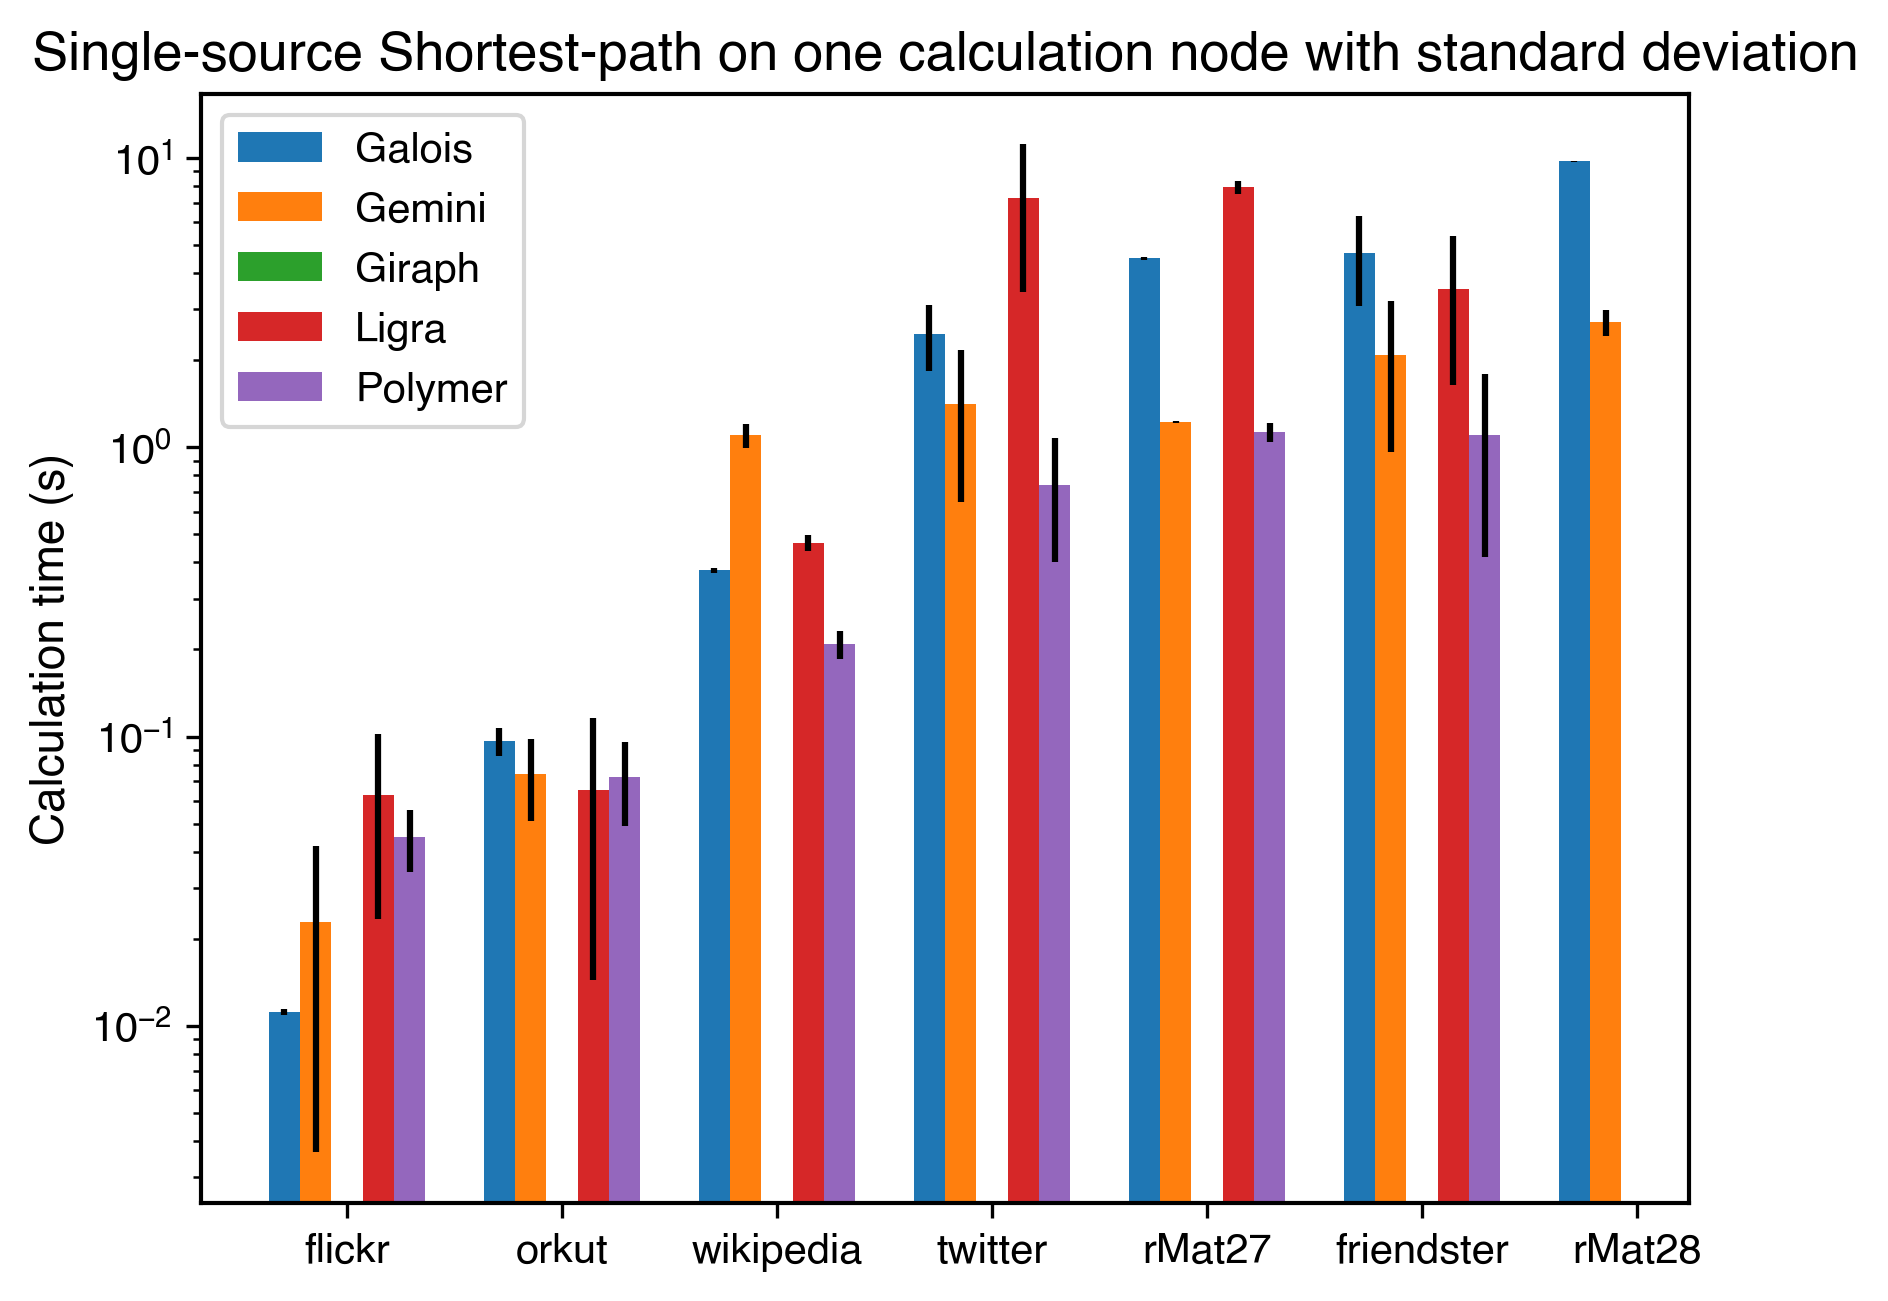
\includegraphics[width=\linewidth]{../../plots/singleNodeSSSP_calcTime.png}
		\caption{Calculation times for SSSP on a single node}
		\label{fig:singleNodeSSSP_calc}
	\end{subfigure}
	\hfil
	\begin{subfigure}{0.3\textwidth}
		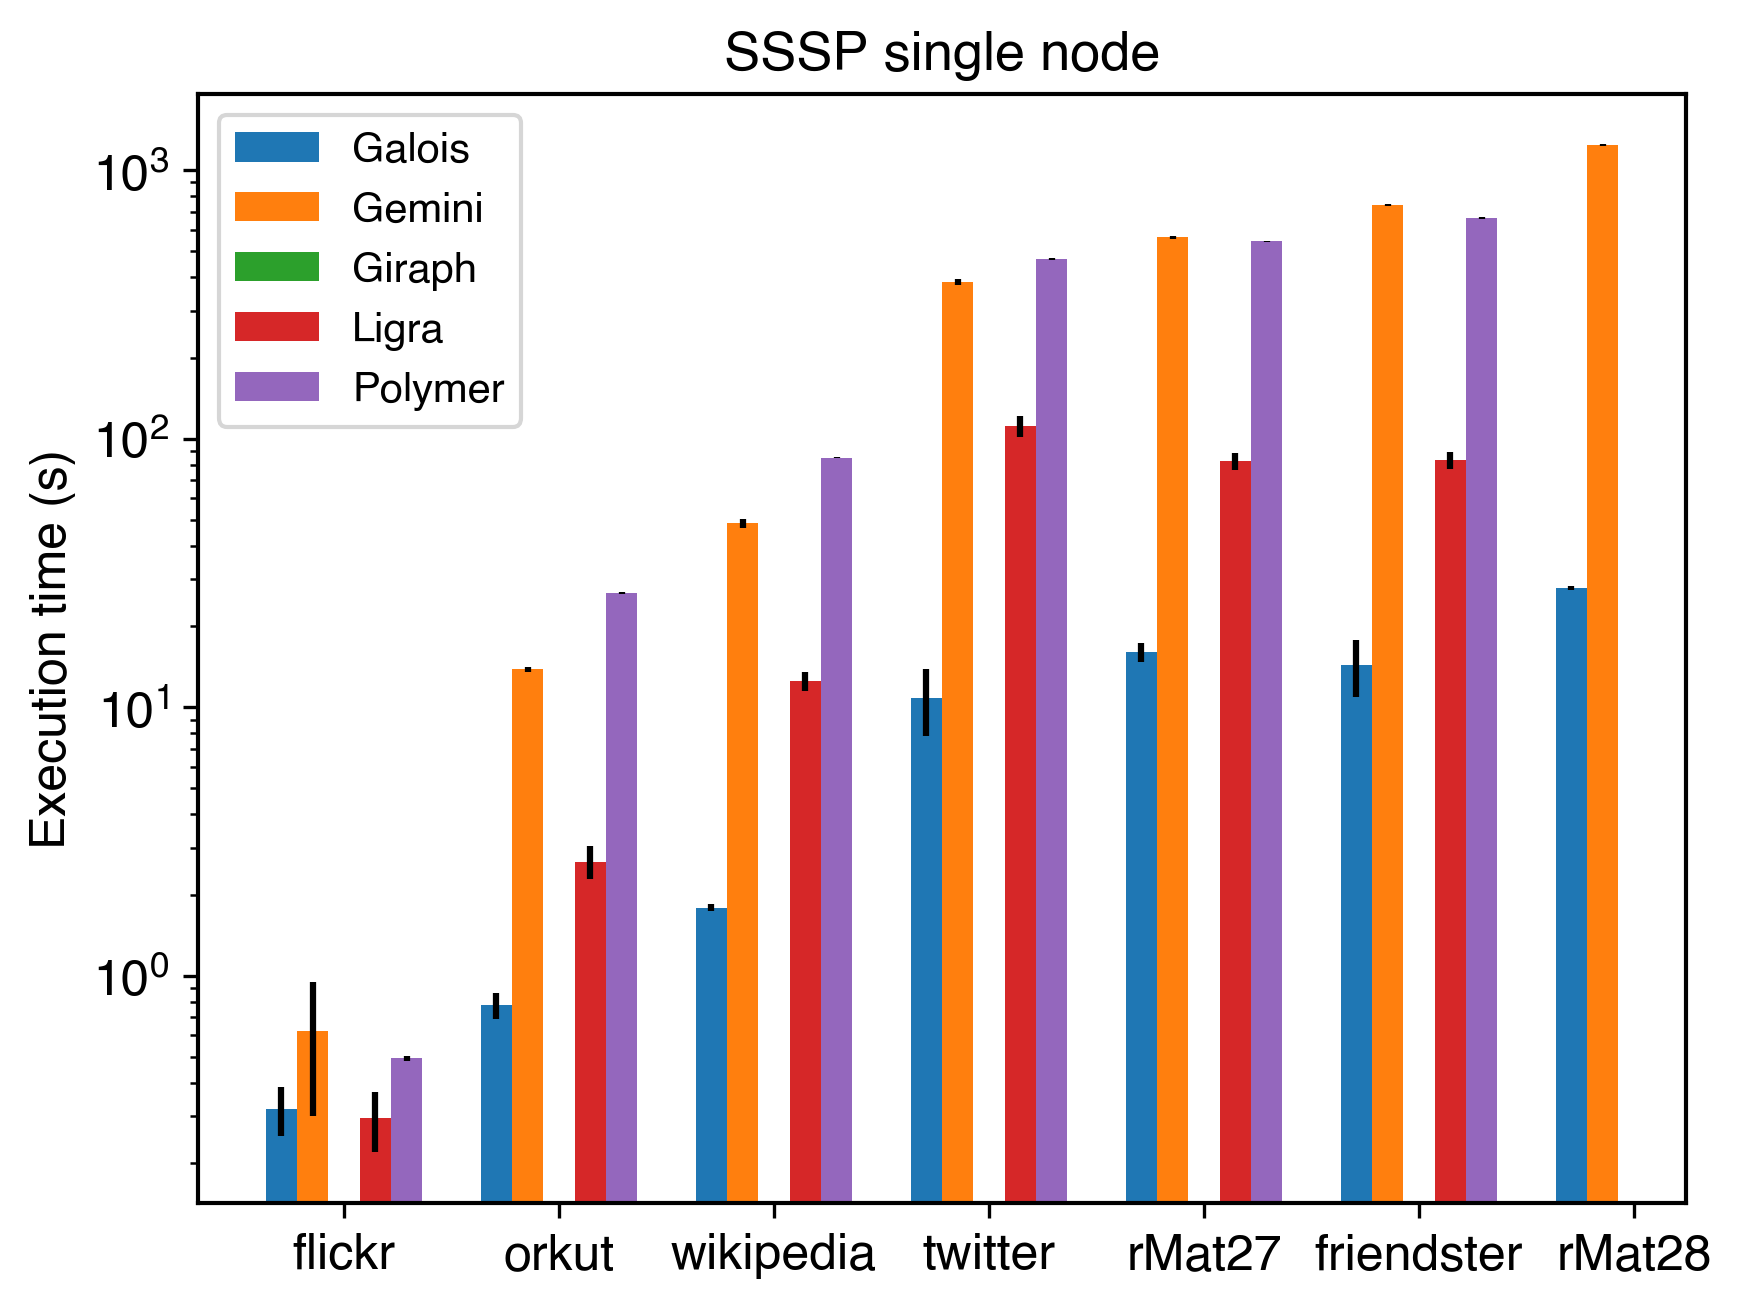
\includegraphics[width=\linewidth]{../../plots/singleNodeSSSP_execTime.png}
		\caption{Execution times for SSSP on a single node}
		\label{fig:singleNodeSSSP_exec}
	\end{subfigure}
	\hfil
	\begin{subfigure}{0.3\textwidth}
		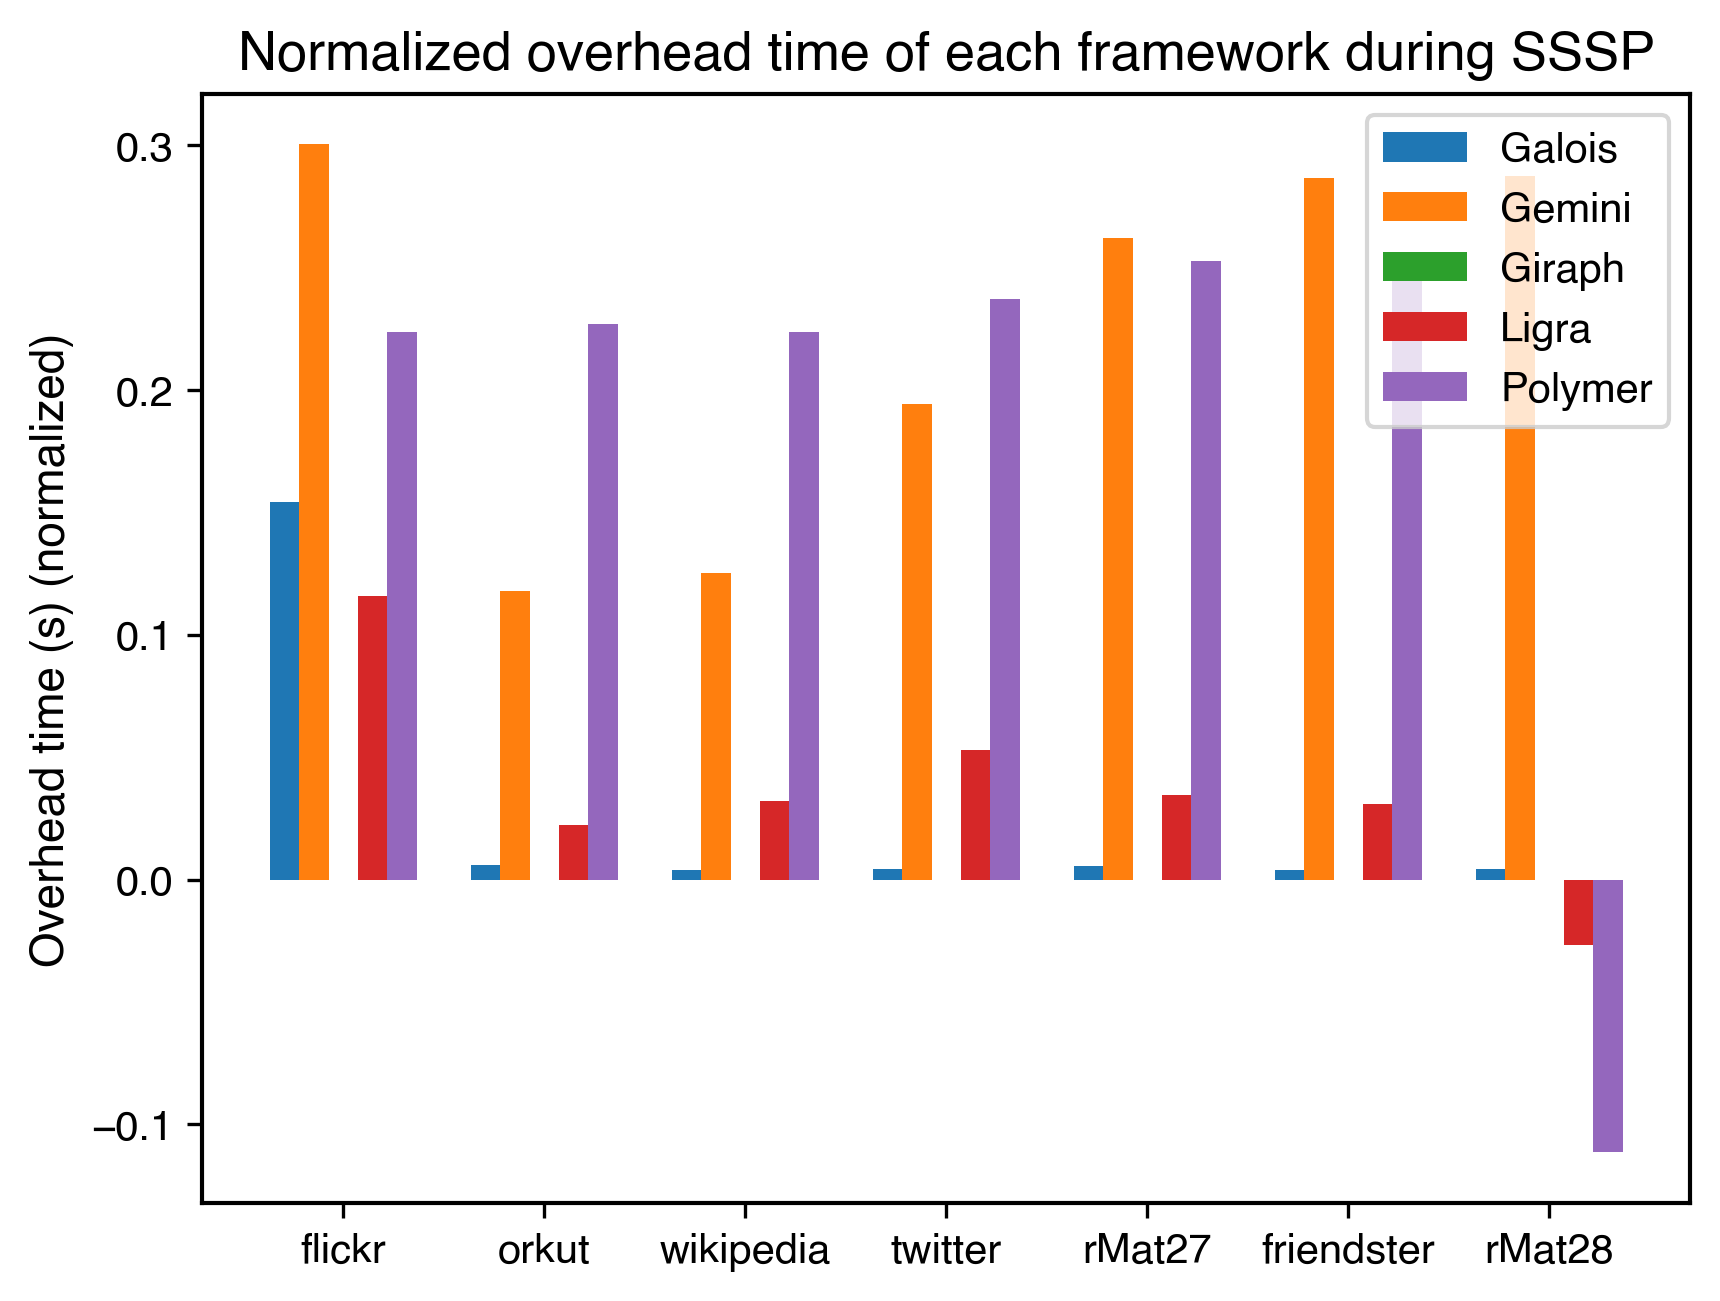
\includegraphics[width=\linewidth]{../../plots/singleNodeSSSP_overheadTimeNormalized.png}
		\caption{Overhead time normalized by the graph size in million edges}
		\label{fig:singleNodeSSSP_overheadNormalized}
	\end{subfigure}
	\caption{Average times on a single computation node, black bars represent one standard deviation in our testing.
	The runs on rMat28 for Ligra and Polymer failed and the frameworks were unable to complete the task.}
	\label{fig:singleNodeSSSP}
\end{figure}








\subsubsection{Distributed}

\begin{figure}
	\centering
	\begin{subfigure}{\columnwidth}
		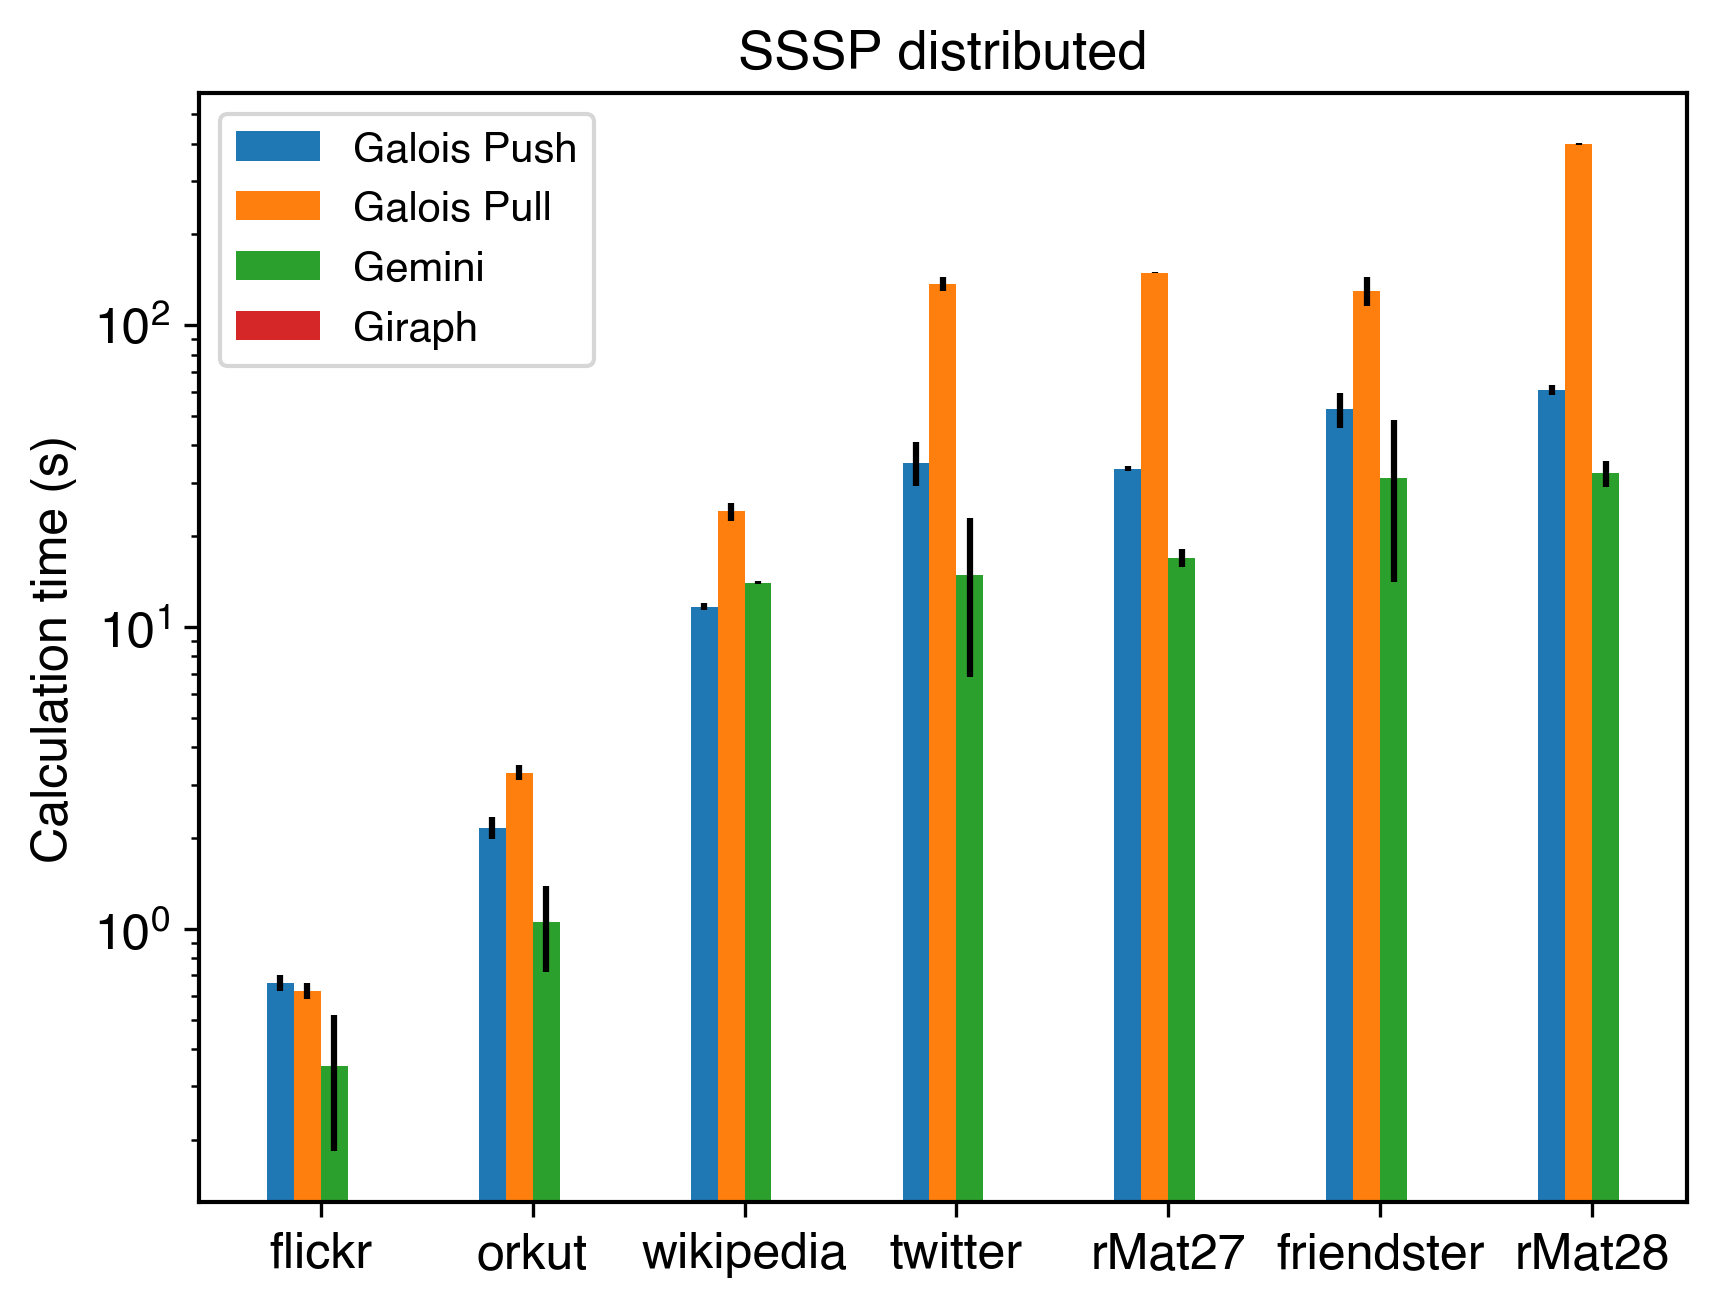
\includegraphics[width=\linewidth]{../../plots/distributedSSSP_calcTime.png}
		\caption{Calculation times for distributed SSSP}
		\label{fig:distributedSSSP_calc}
	\end{subfigure}
	\begin{subfigure}{\columnwidth}
		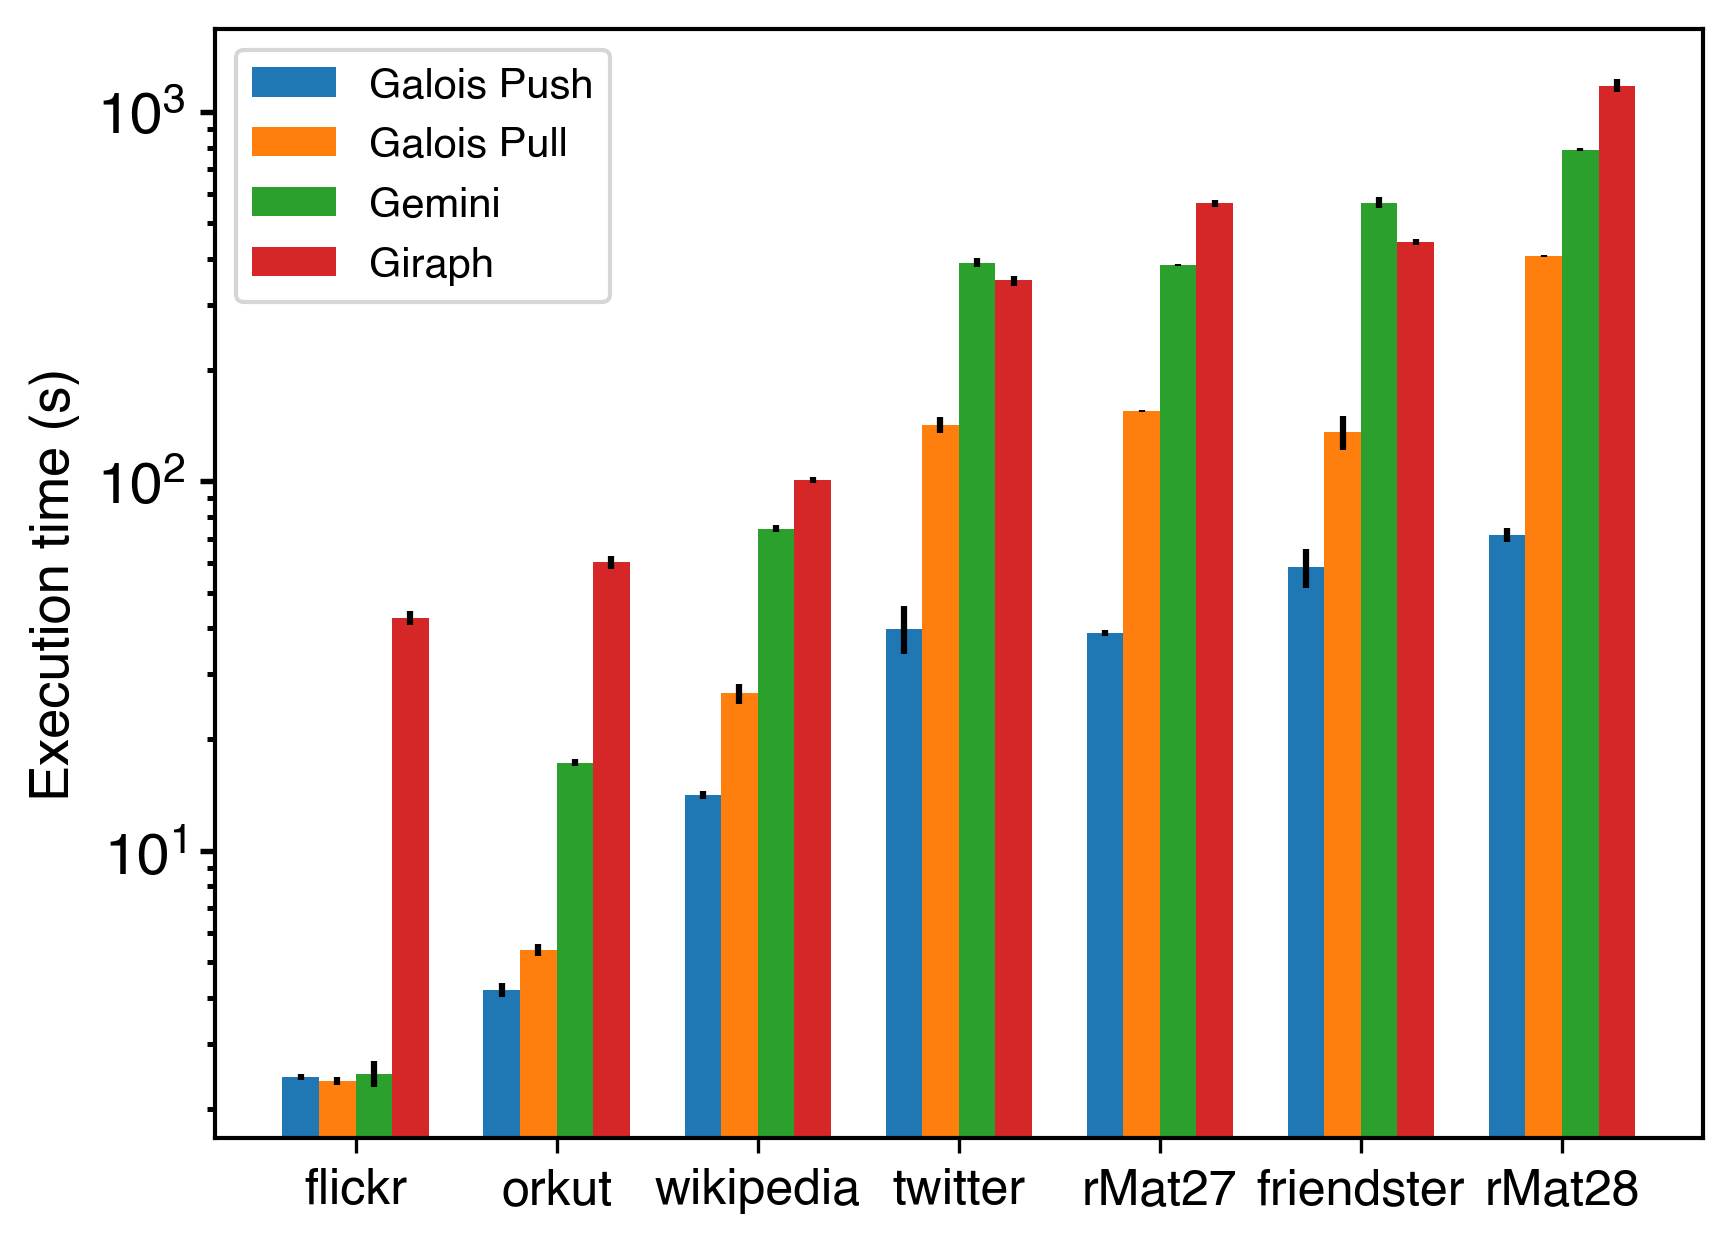
\includegraphics[width=\linewidth]{../../plots/distributedSSSP_execTime.png}
		\caption{Execution times for distributed SSSP}
		\label{fig:distributedSSSP_exec}
	\end{subfigure}
	\caption{Average times on the distributed cluster, black bars represent one standard deviation in our testing.}
	\label{fig:distributedSSSP}
\end{figure}

\begin{figure}
	\centering
	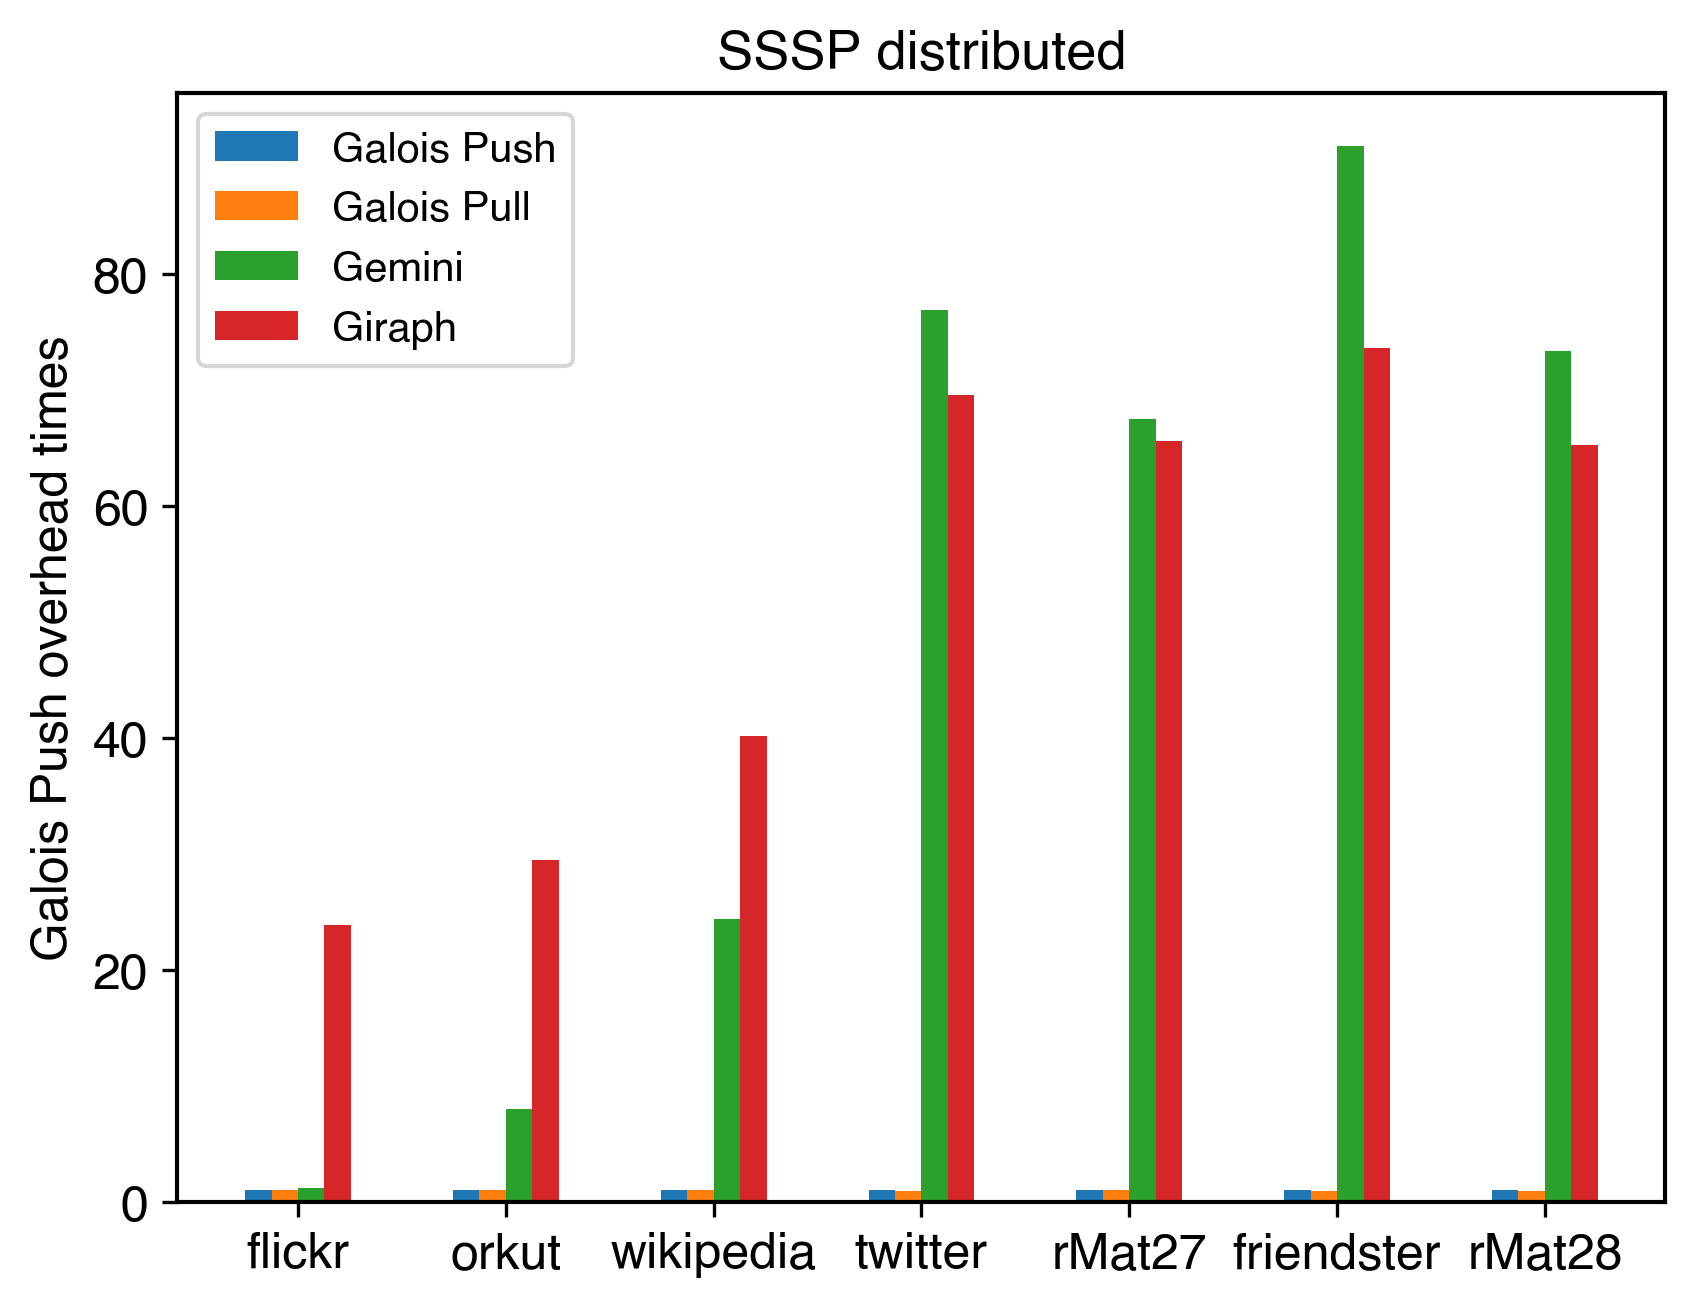
\includegraphics[width=\linewidth]{../../plots/distributedSSSP_overheadTimeNormalizedToGalois.png}
	\caption{Distributed Single-Source Shortest-Paths overhead times of each framework normalized by the overhead time of Galois Push}
	\label{fig:distributedSSSP_overhead}
\end{figure}

Moving on to the distributed cluster, \autoref{fig:distributedSSSP} shows the benchmark results as calculation and execution times. 

Comparing the two Galois implementations, we find the calculation and execution times to be similar on smaller graphs and Push being the superior implementation for SSSP on larger data sets. Galois Pull being anywhere from just as fast to 3.5$\times$ slower on real-world data sets compared to the Push variant. The synthetic graphs are more extreme, execution times are close to 4$\times$ (rMat27) and 5$\times$ (rMat28) longer.

Both Galois implementations have significantly smaller execution times compared to Gemini or Giraph on all graphs, see \autoref{tbl:ssspexec}.
You can see Gemini being worse by at least a factor of 4 compared to Galois Push on all graphs except flickr.
Giraph's execution times in comparison to this are even worse, taking at least 7$\times$ longer than Galois Push on all graphs.

Evidently, Galois Push is the fastest algorithm in our lineup on 6 out of 7 graphs. With the exception being flickr, where Galois Push takes negligibly longer than the Pull counterpart. 



\begin{table}
\renewcommand{\arraystretch}{1.3}
\centering
\caption{Distributed SSSP Execution Times Relative to Galois Push}
\begin{tabular}{crrrr}
\hline
\bf{Data Set}&Galois Push&Galois Pull&Gemini&Giraph\\\hline
flickr&1.0&0.97&1.02&17.46\\
orkut&1.0&1.28&4.12&14.38\\
wikipedia&1.0&1.88&5.26&7.11\\
twitter&1.0&3.56&9.79&8.76\\
rMat27&1.0&3.98&9.91&14.52\\
friendster&1.0&2.32&9.72&7.59\\
rMat28&1.0&5.70&11.07&16.5\\\hline
\end{tabular}
\label{tbl:ssspexec}
\end{table}



When taking a closer look at Giraph, it seems to not cope well with synthetic data sets. Analyzing the computation times in \autoref{fig:distributedSSSP_calc}, we see that it is the fastest framework on our real-world graphs. And that with a considerable margin of other frameworks always taking at least 50\% longer (lower bound here is Gemini on flickr) up to Galois Pull needing 18$\times$ more time on wikipedia.  
On both synthetic graphs however, Giraph is actually the slowest to compute. Giraph requires 12$\times$ or even 15$\times$ the computation time of Gemini on rMat27 or rMat28 respectively.

While Giraph's computation times are very competitive, when comparing the execution times in \autoref{fig:distributedSSSP_exec} we see that Giraph is actually the slowest framework on 5 out of 7 graphs. For the other two, namely twitter and friendster, Giraph is second slowest with only Gemini taking longer to complete.

Giraph and Gemini's very long execution times are only due to their overhead being many orders of magnitude larger than Galois overhead (\autoref{fig:distributedSSSP_overhead}).
Overhead for Gemini is greater than that of Galois on every graph. From just a 20\% increase on flickr up to friendster, where the overhead is 90$\times$ that of Galois Push.
For Giraph the overhead times are not as extreme but still generally worse. Even on flickr, Giraph's overhead time is already 23$\times$ that of Galois. On friendster, where Gemini was worst, Giraph \emph{only} requires 73$\times$ the overhead time of Galois.



\subsubsection{Single-Node vs. Distributed}
TODO
\begin{itemize}
	\item GaloisPush vs Galois CPU // Galois Pull verliert bei Dist.
	\item Giraph vs. Giraph
	\item Gemini vs Gemini
\end{itemize}




%!TEX root=../../main.tex

\subsection{Breadth-first search}
\subsubsection{Single-Node}
\todo{Hier fehlt noch Giraph, daher noch keine vollständige Auswertung.}


In these figures, Galois with 96 threads is shown. Again, we show the impact of Galois' thread count in \autoref{sec:galois_speedup}.
\begin{figure*}
	\begin{subfigure}{0.3\textwidth}
		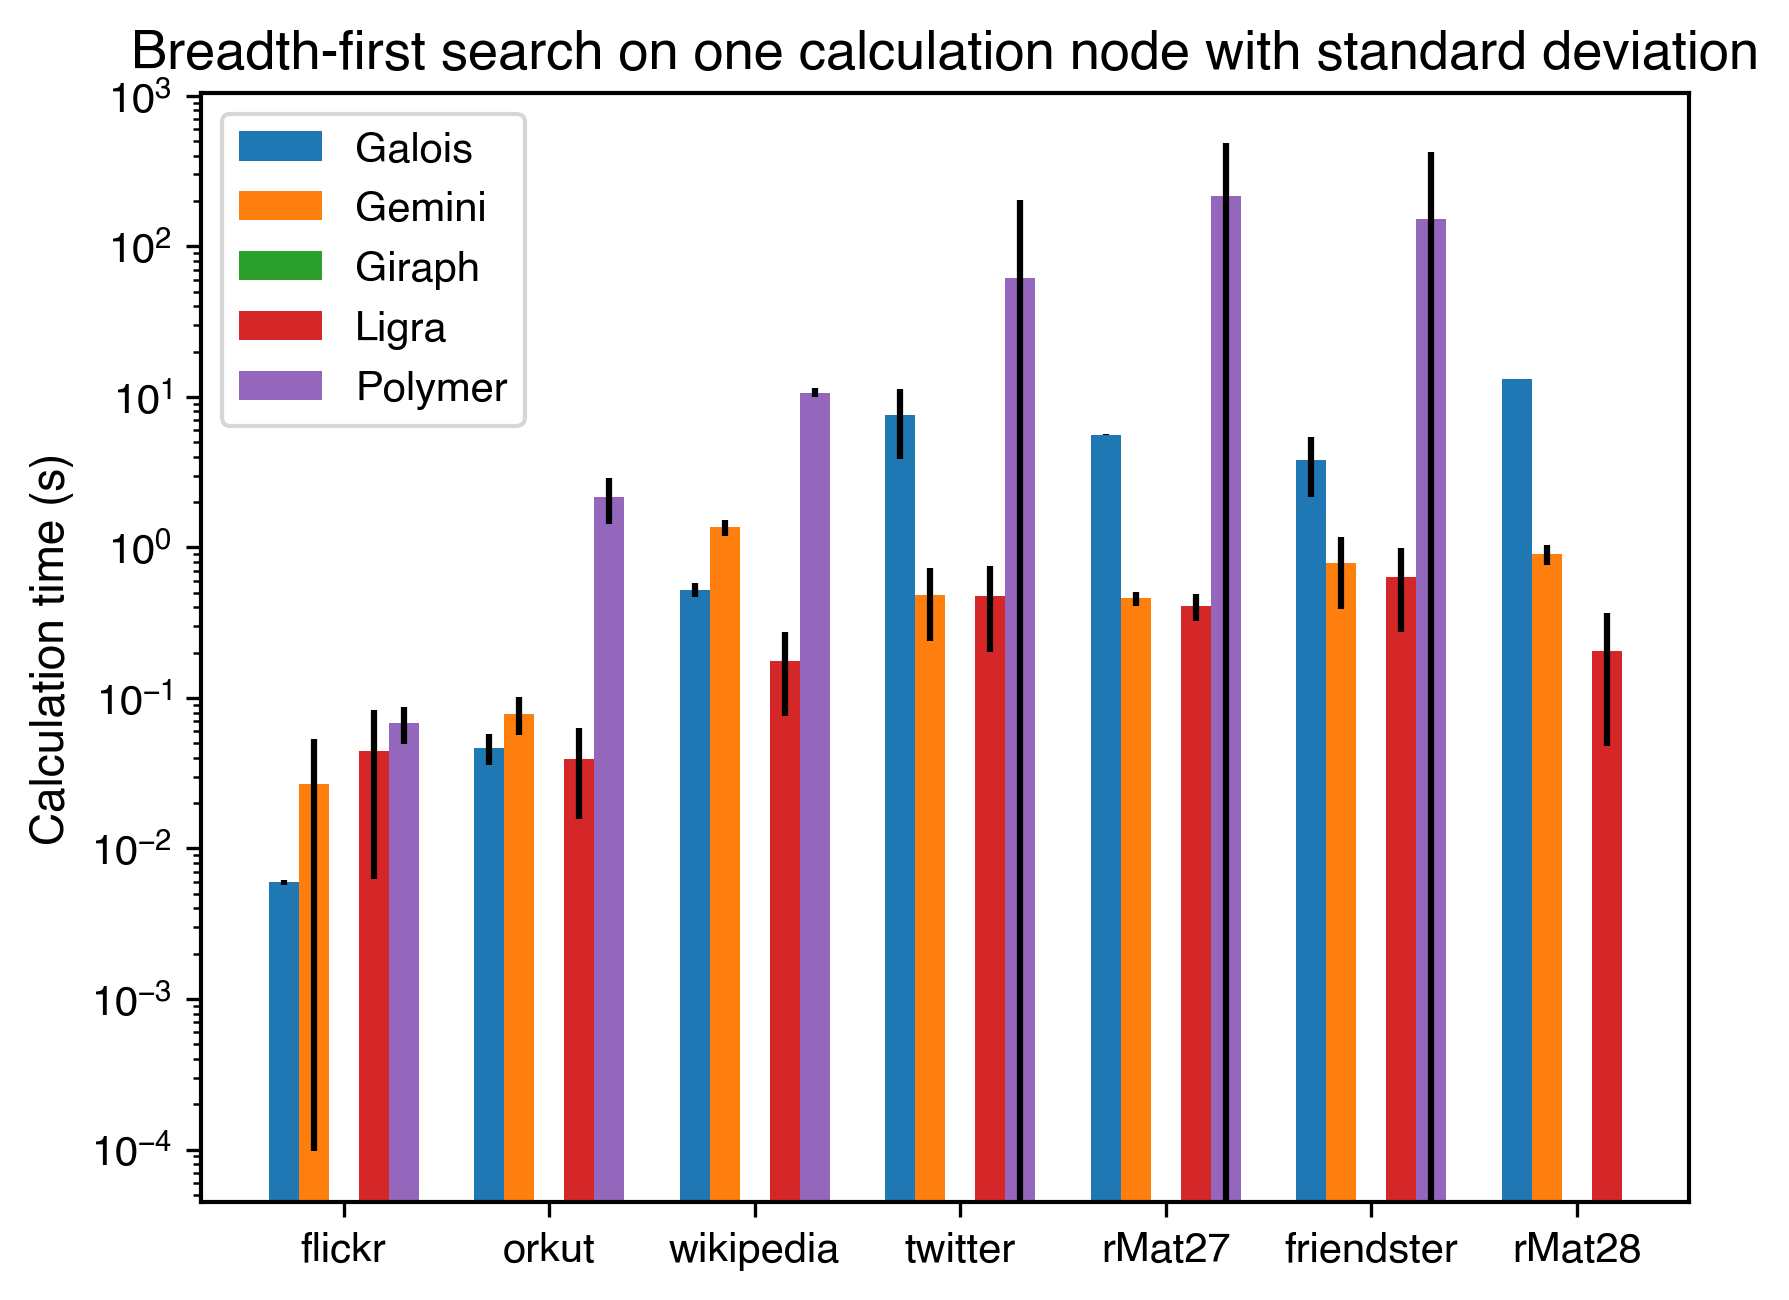
\includegraphics[width=\linewidth]{../../plots/singleNodeBFS_calcTime.png}
		\caption{Calculation times for BFS on a single node}
		\label{fig:singleNodeBFS_calc}
	\end{subfigure}
	\hfil
	\begin{subfigure}{0.3\textwidth}
		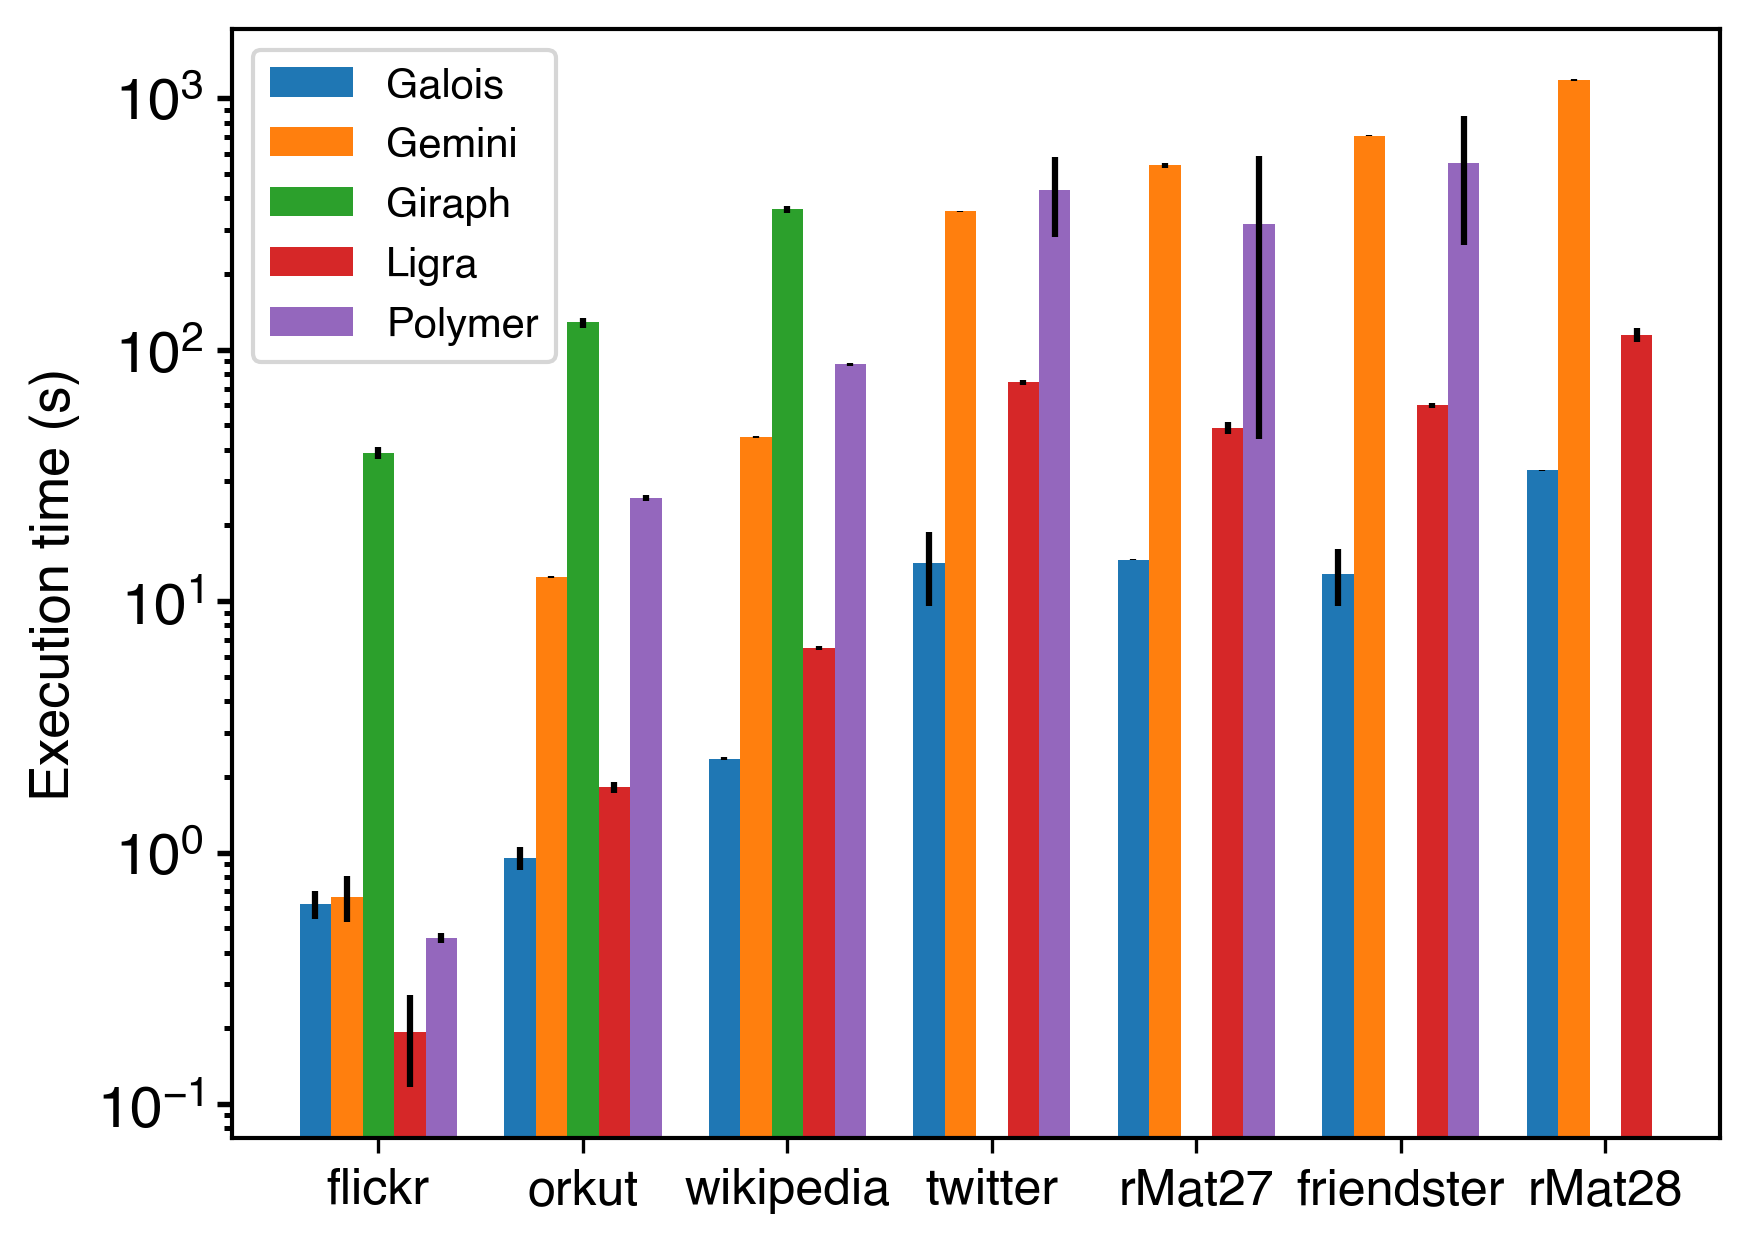
\includegraphics[width=\linewidth]{../../plots/singleNodeBFS_execTime.png}
		\caption{Execution times for BFS on a single node}
		\label{fig:singleNodeBFS_exec}
	\end{subfigure}
	\hfil
	\begin{subfigure}{0.3\textwidth}
		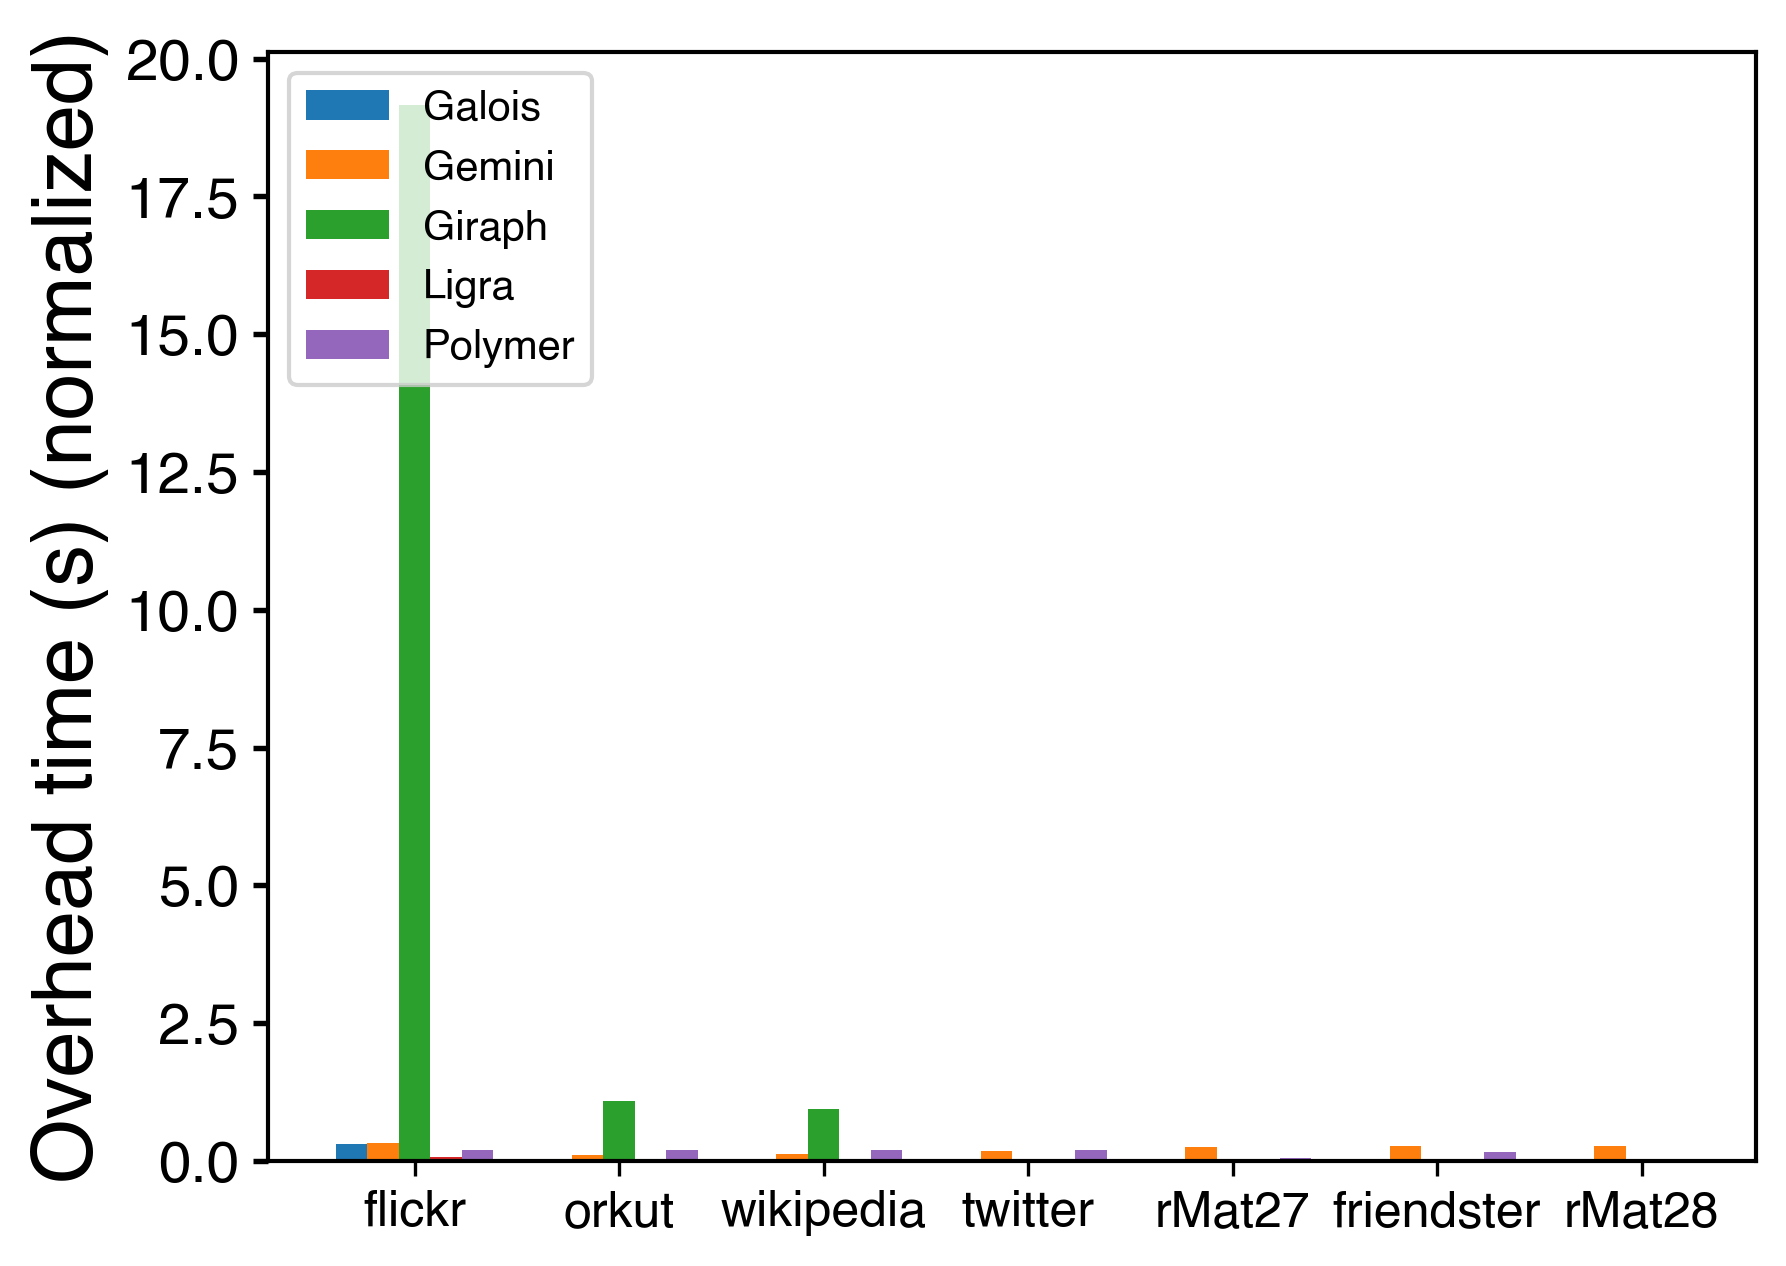
\includegraphics[width=\linewidth]{../../plots/singleNodeBFS_overheadTimeNormalized.png}
		\caption{Overhead time normalized by the graph size in million edges}
		\label{fig:singleNodeBFS_overheadNormalized}
	\end{subfigure}

	\caption{Average times on a single computation node, black bars represent one standard deviation in our testing}
\end{figure*}



\subsubsection{Distributed}
\begin{figure}
	\begin{subfigure}{\columnwidth}
		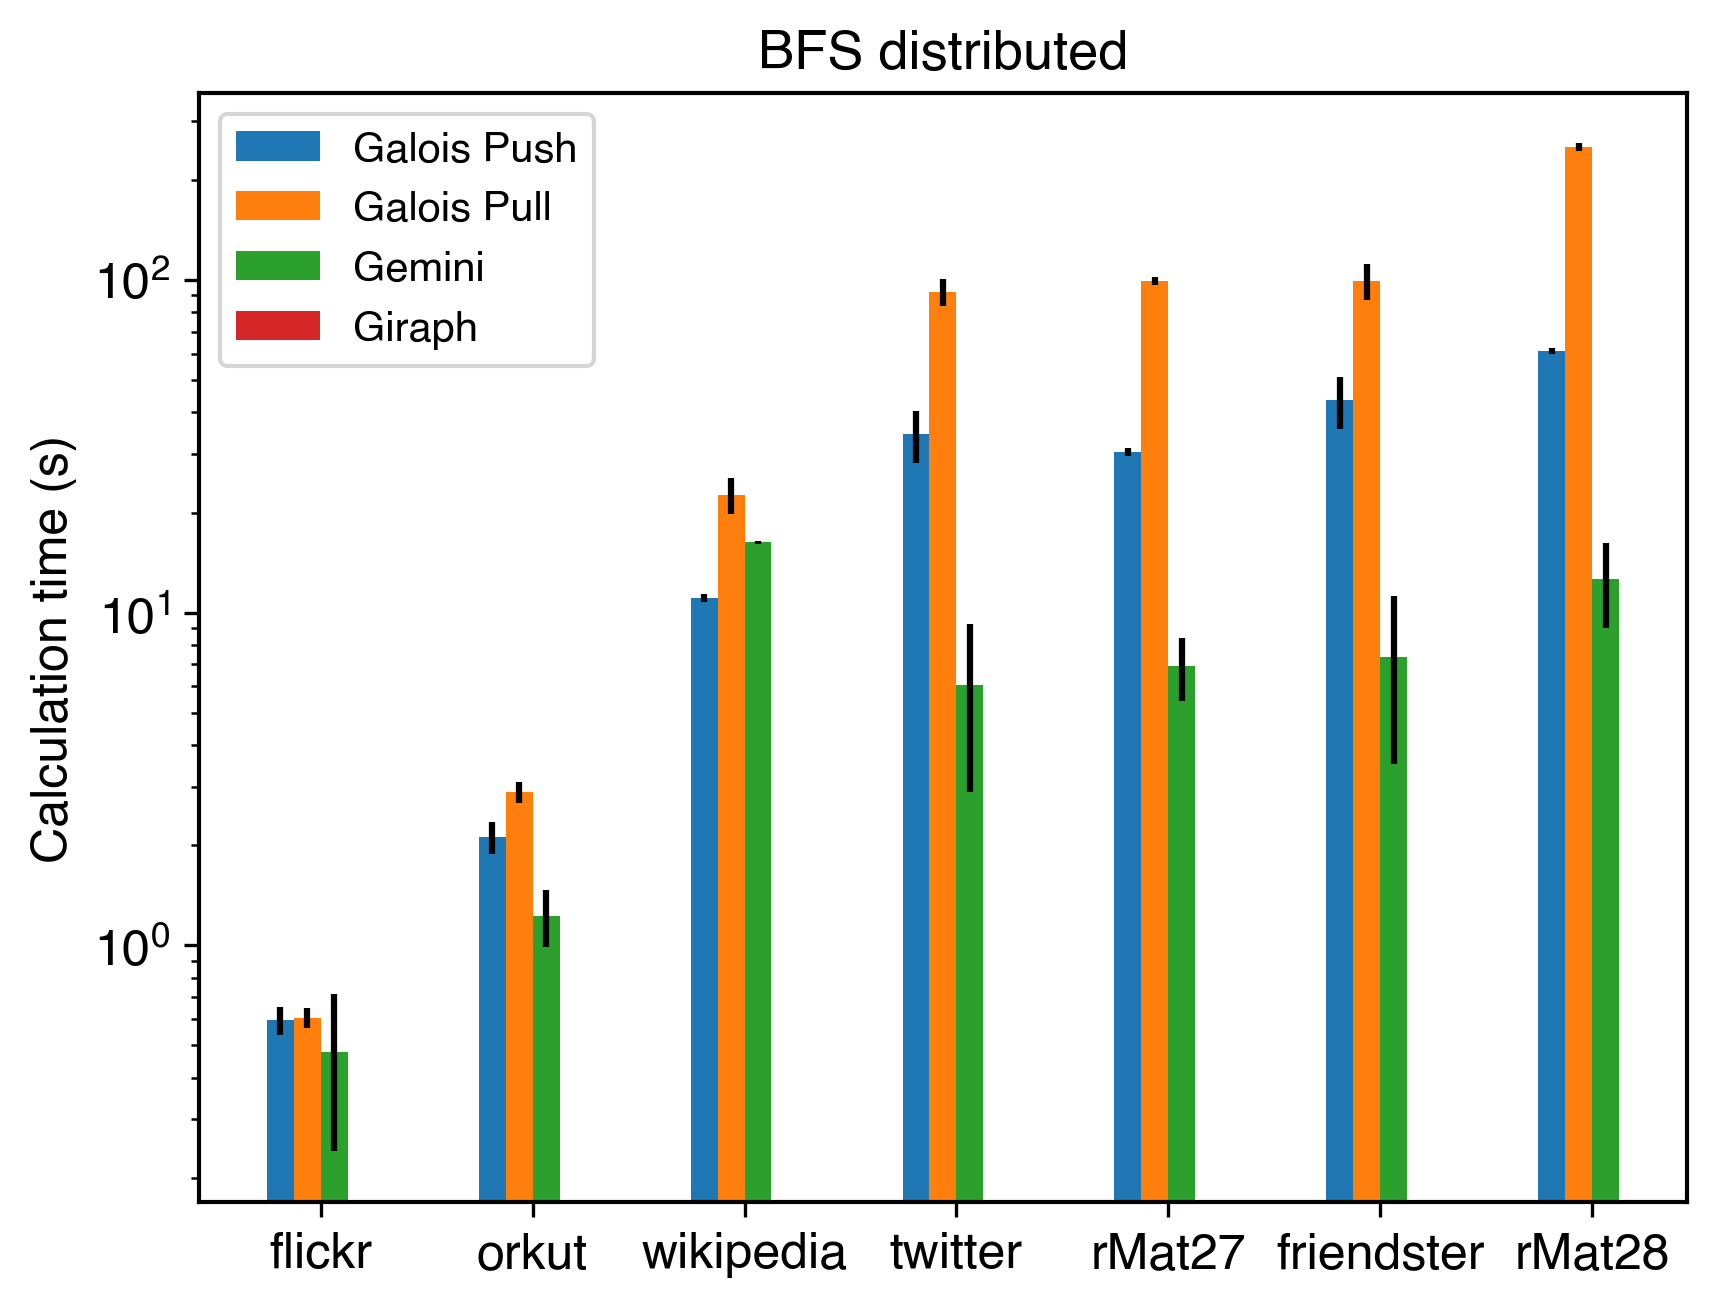
\includegraphics[width=\linewidth]{../../plots/distributedBFS_calcTime.png}
		\caption{Calculation times for distributed BFS}
		\label{fig:distributedBFS_calc}
	\end{subfigure}
	% \hfil
	\begin{subfigure}{\columnwidth}
		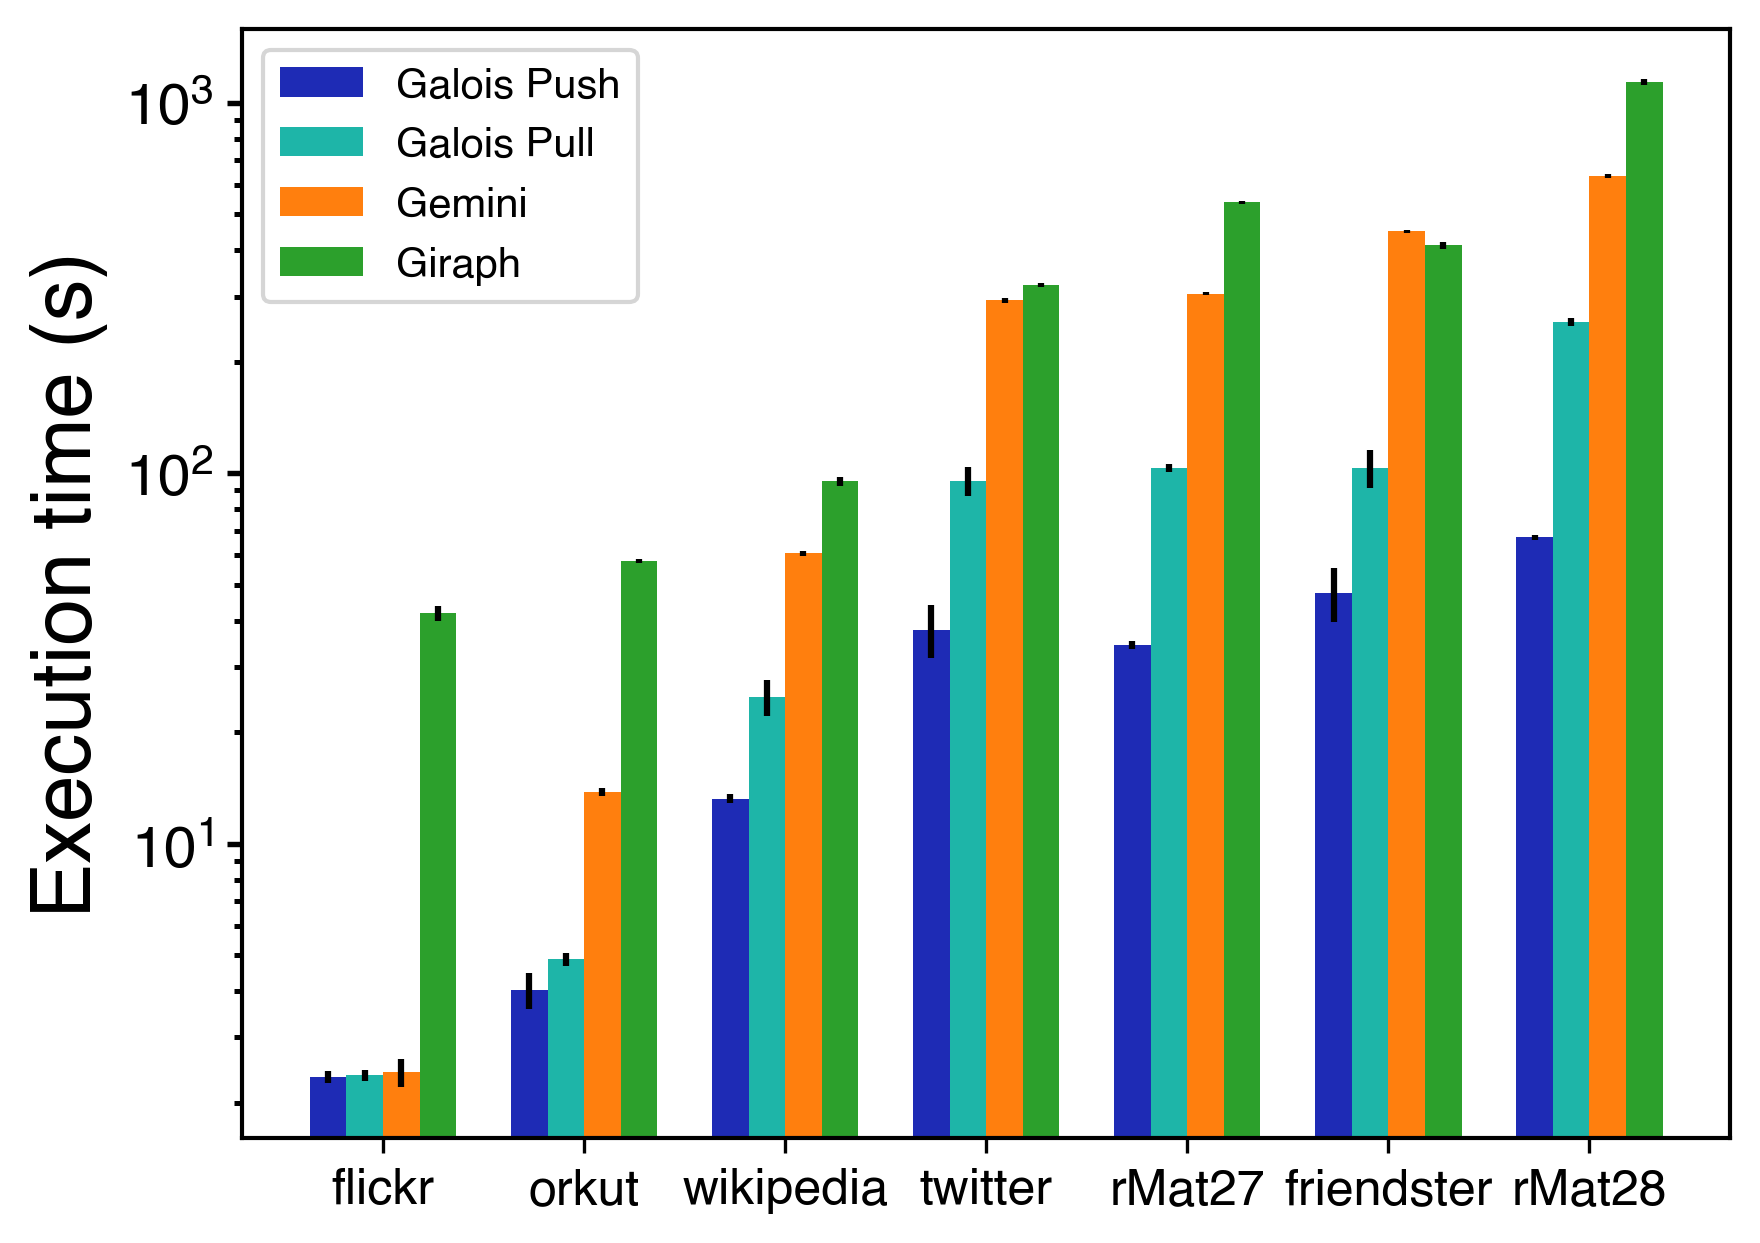
\includegraphics[width=\linewidth]{../../plots/distributedBFS_execTime.png}
		\caption{Execution times for distributed BFS}
		\label{fig:distributedBFS_exec}
	\end{subfigure}
	% \hfil
	% \begin{subfigure}{0.3\textwidth}
	% 	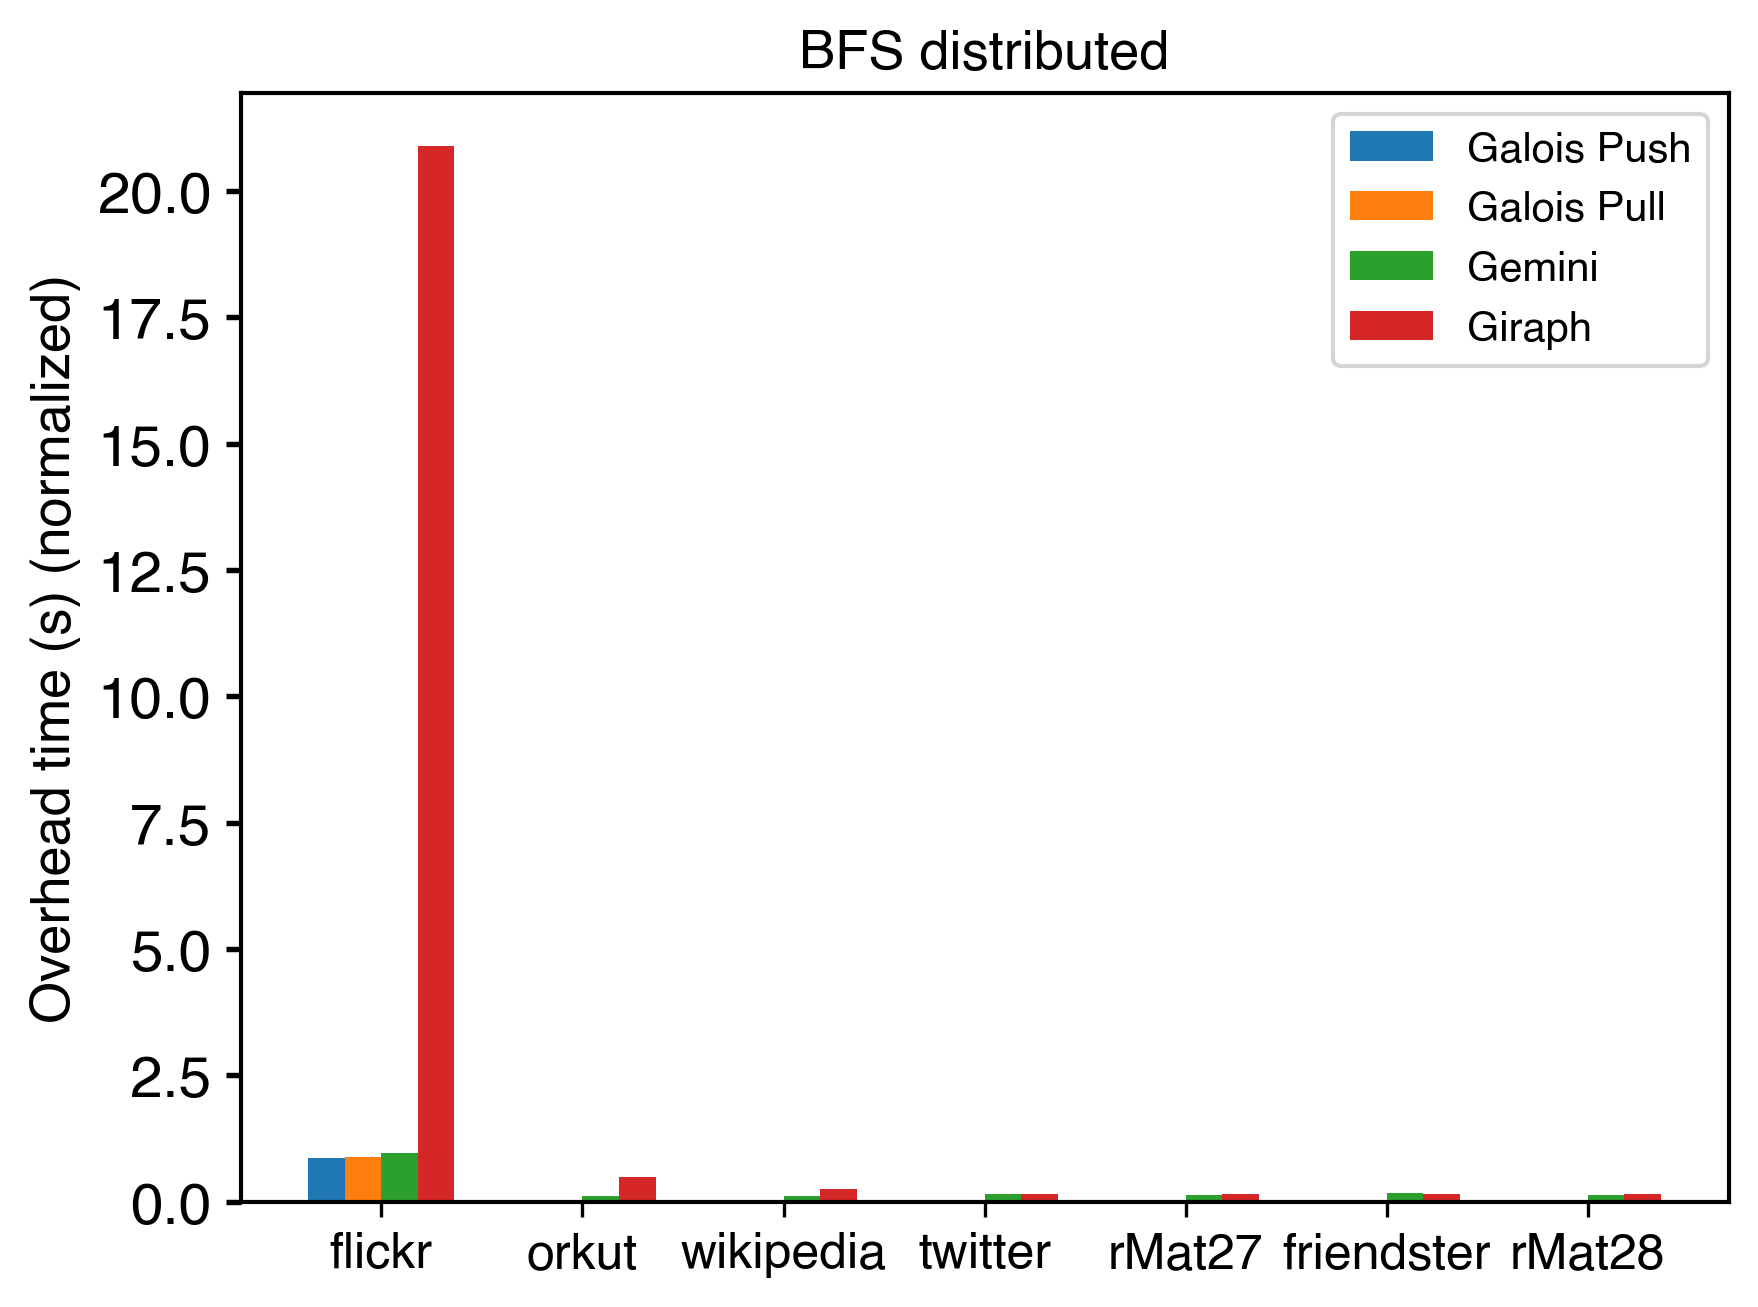
\includegraphics[width=\linewidth]{../../plots/distributedBFS_overheadTimeNormalized.png}
	% 	\caption{Overhead time normalized by the graph size in million edges}
	% 	\label{fig:distributedBFS_overheadNormalized}
	% \end{subfigure}
	\caption{Average times on the distributed cluster, black bars represent one standard deviation in our testing}
	\label{fig:distributedBFS}
\end{figure}
For both the calculation and the execution times, Breadth-First Search shows similar behaviour as the distributed SSSP test case. This is expected since both are graph traversal algorithms starting in one source vertex.
Hence, calculation complexity for each vertex and communication overhead is similar.
All measurements can be seen in \autoref{fig:distributedBFS}.

First, the calculation times in \autoref{fig:distributedBFS_calc}. It shows Giraph having the shortest calculation times on the real-world graphs, while Giraph's calculatin times on both rMat27 and rMat28 are the worst of all frameworks.

Comparing the execution times in \autoref{fig:distributedBFS_exec} results in the same findings as with SSSP.
While Gemini can compete with Galois on the small flickr graph, moving to larger data sets shows the worse performance of Gemini compared to Galois.

Much like when running SSSP, Giraph is slowest on all but one graph. Only on friendster is Gemini marginally slower, which was also the case for SSSP.

Both Galois implementations are again similar to the behaviour on SSSP.
Galois Push is generally faster than the Pull alternative while both Push and Pull versions are faster than Gemini and Giraph across all graphs.
This makes Galois Push the clear winner for distributed BFS.



%!TEX root=../../main.tex


\subsubsection{PageRank}
In this section we compare the PageRank performance of the various frameworks. As usual we begin with the single-node performance and finish by discussing the distributed variants.

\paragraph{Single-Node}
Ligra and Polymer support both regular and Delta-PageRank variants.
Ligra's regular PR implementation is faster on 4 of 7 graphs. If the regular version is slower than delta, that is only by a small difference. Explicitly, regular is slower than delta by a range of 6\% to 19\%\ on twitter, rMat27 or friendster. For the other graphs, the delta version is slower by a far greater margin of 13\% to 68\%.
Hence, we only show the results of Ligra's regular PageRank implementation in our evaluation.
For Polymer we found the delta version to be faster on all graphs except rMat28. Delta-PR is on average 15\%\ faster on the first six graphs, while only being 0.3\%\ slower on rMat28.
Thus, the following only shows Polymer's faster Delta-PR implementation.
Giraph required more than the available 250 GB of RAM on any graph larger than wikipedia, hence all of Giraph's results for the larger graphs are missing here.
\begin{figure*}
	\hfil
	\begin{subfigure}{0.32\textwidth}
		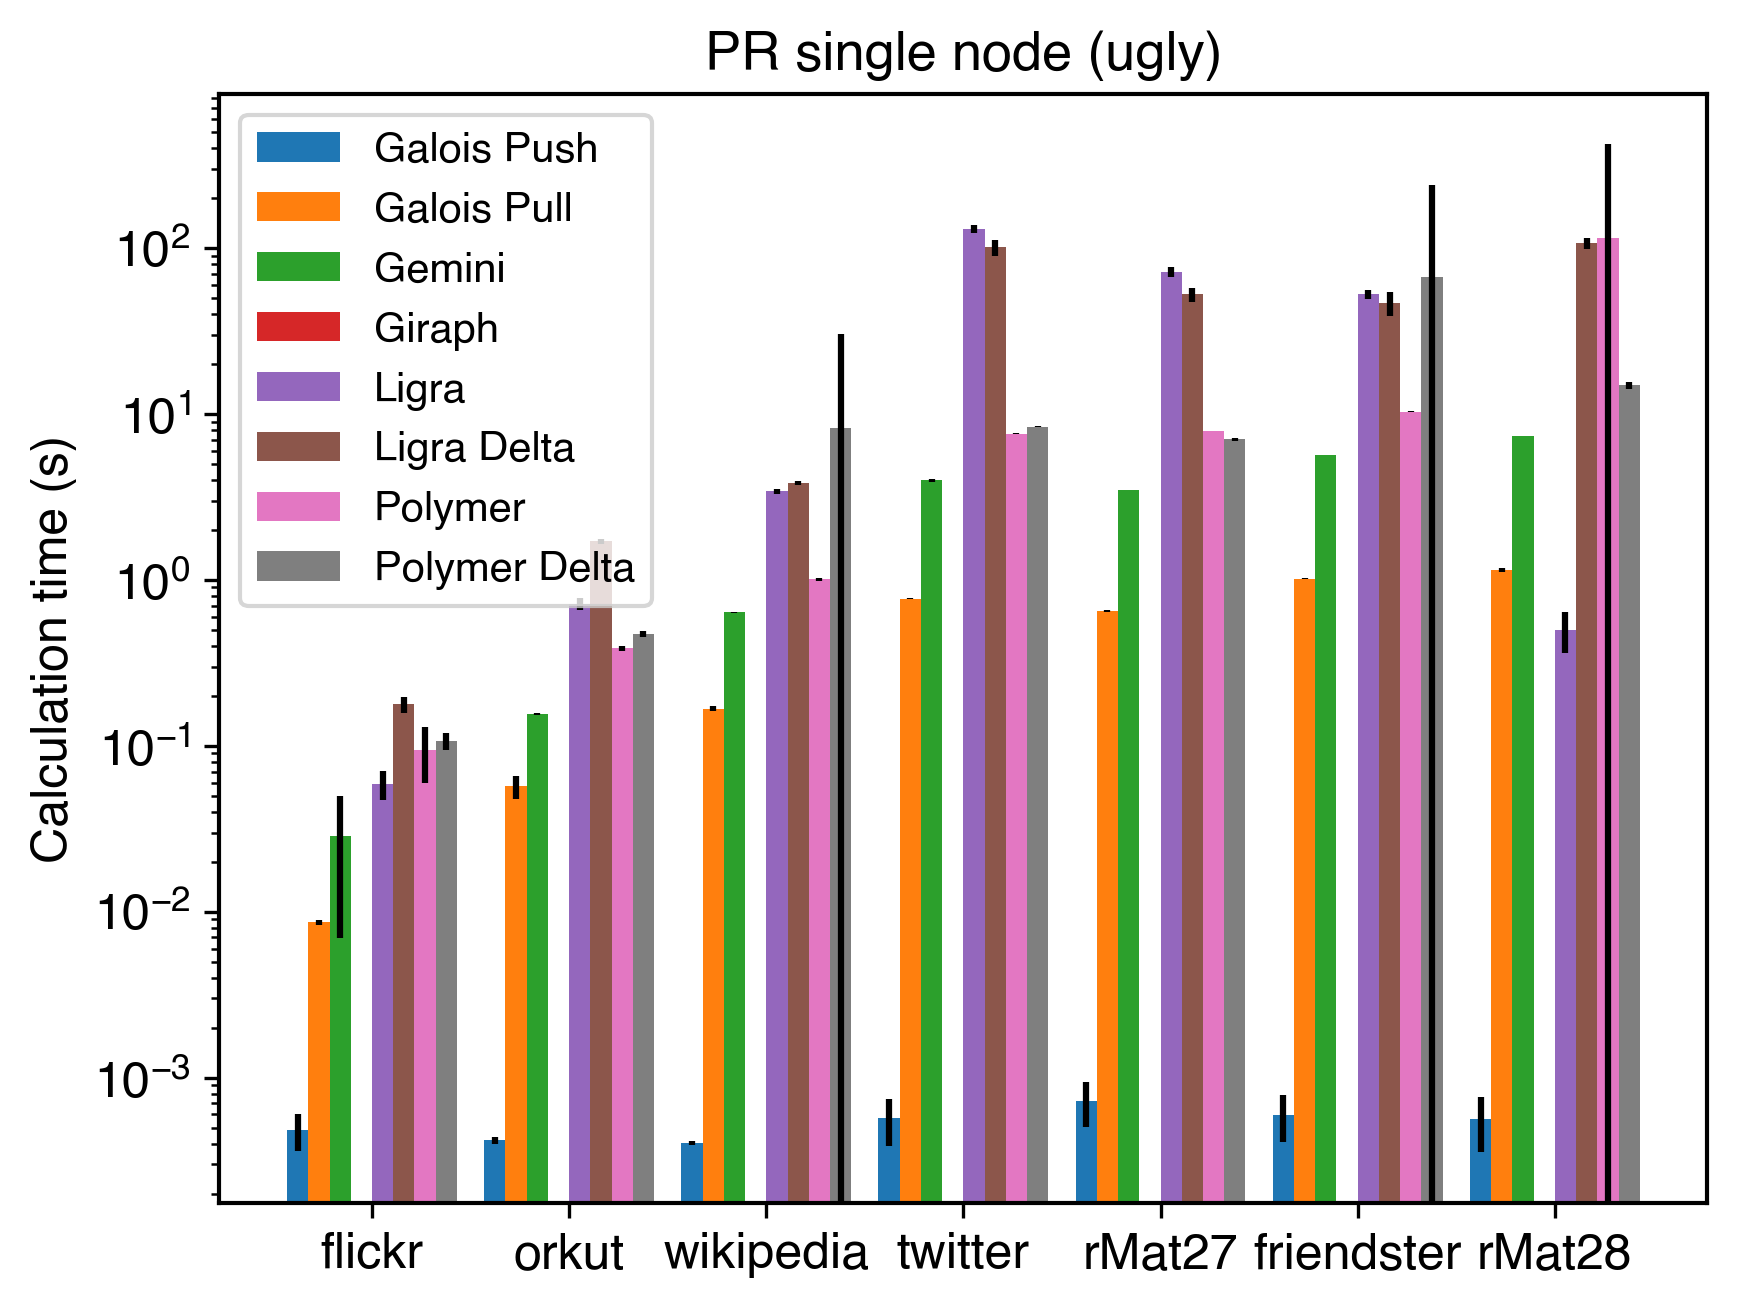
\includegraphics[width=\linewidth]{../../plots/singleNodePR_calcTime.png}
		\caption{Calculation time}
		\label{fig:singleNodePR_calc}
	\end{subfigure}
	\hfil
	\begin{subfigure}{0.32\textwidth}
		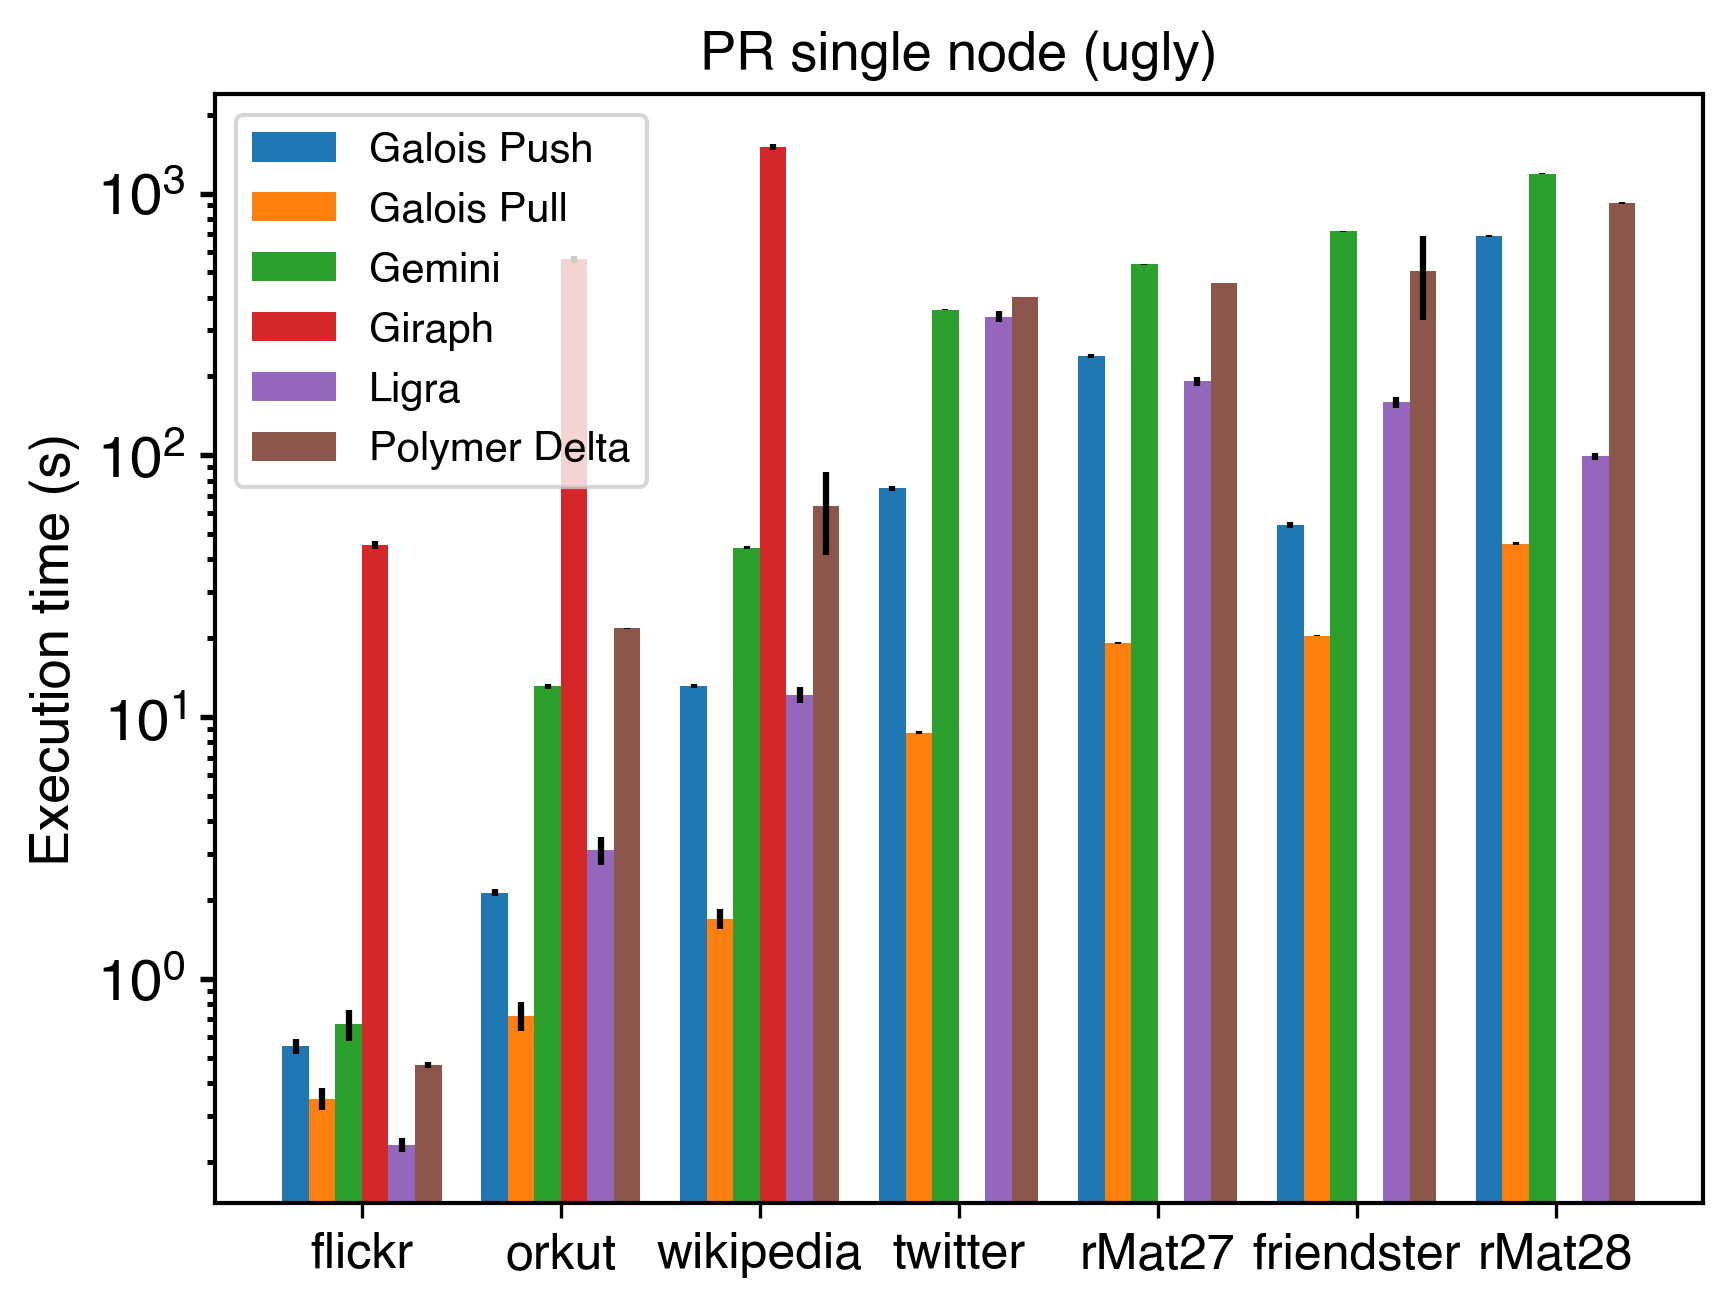
\includegraphics[width=\linewidth]{../../plots/singleNodePR_execTime.png}
		\caption{Execution time}
		\label{fig:singleNodePR_exec}
	\end{subfigure}
	\hfil
	\begin{subfigure}{0.32\textwidth}
		\includegraphics[width=\linewidth]{../../plots/singleNodePR_overheadTIme.png}
		\caption{Overhead}
		\label{fig:singleNodePR_overhead}
	\end{subfigure}
	\hfil
	\caption{Average times for PR on a single computation node, black bars represent one standard deviation in our testing}
	\label{fig:singleNodePR}
\end{figure*}

The calculation times show some odd behaviour of Galois Push. The required time is less than 1ms, regardless of the graph (cf. \autoref{fig:singleNodePR_calc}). Meanwhile there was no output produced, that would indicate any kind of error. These results would make the calculation times of Galois Push the smallest on all graphs, with a difference of at least one order of magnitude. However, we are very suspicious of these results and thus exclude the calculation time for Galois Push in further comparisons. Because the execution time of Galois Push is always considerably longer than the execution time of Galois Pull (cf. \autoref{fig:singleNodePR_calc}). This leads us to believe that the output that we used for our measurements contains an error.

For the three graphs on which Giraph computed successfully, it is the slowest framework in both calculation and execution times. And that by a difference of three orders of magnitude in the calculation time and one to two orders of magnitude in execution time (cf \autoref{fig:singleNodePR}). On the larger graphs (i.e. those, where there is no data for Giraph), Gemini and Ligra are always slowest in execution time.
Contrary to this, Galois Pull has the smallest execution times on all graphs except flickr (cf. \autoref{fig:singleNodePR_exec}). Ligra is fastest on flickr, while being second fastest on wikipedia, rMat27 and rMat28. Galois Push is second fastest on orkut and friendster.
Interestingly, the execution time for Ligra is at a maximum for twitter. The required time is steadily decreasing with increasing graph size.



\paragraph{Distributed}
\begin{figure*}
	\hfil
	\begin{subfigure}{0.32\textwidth}
		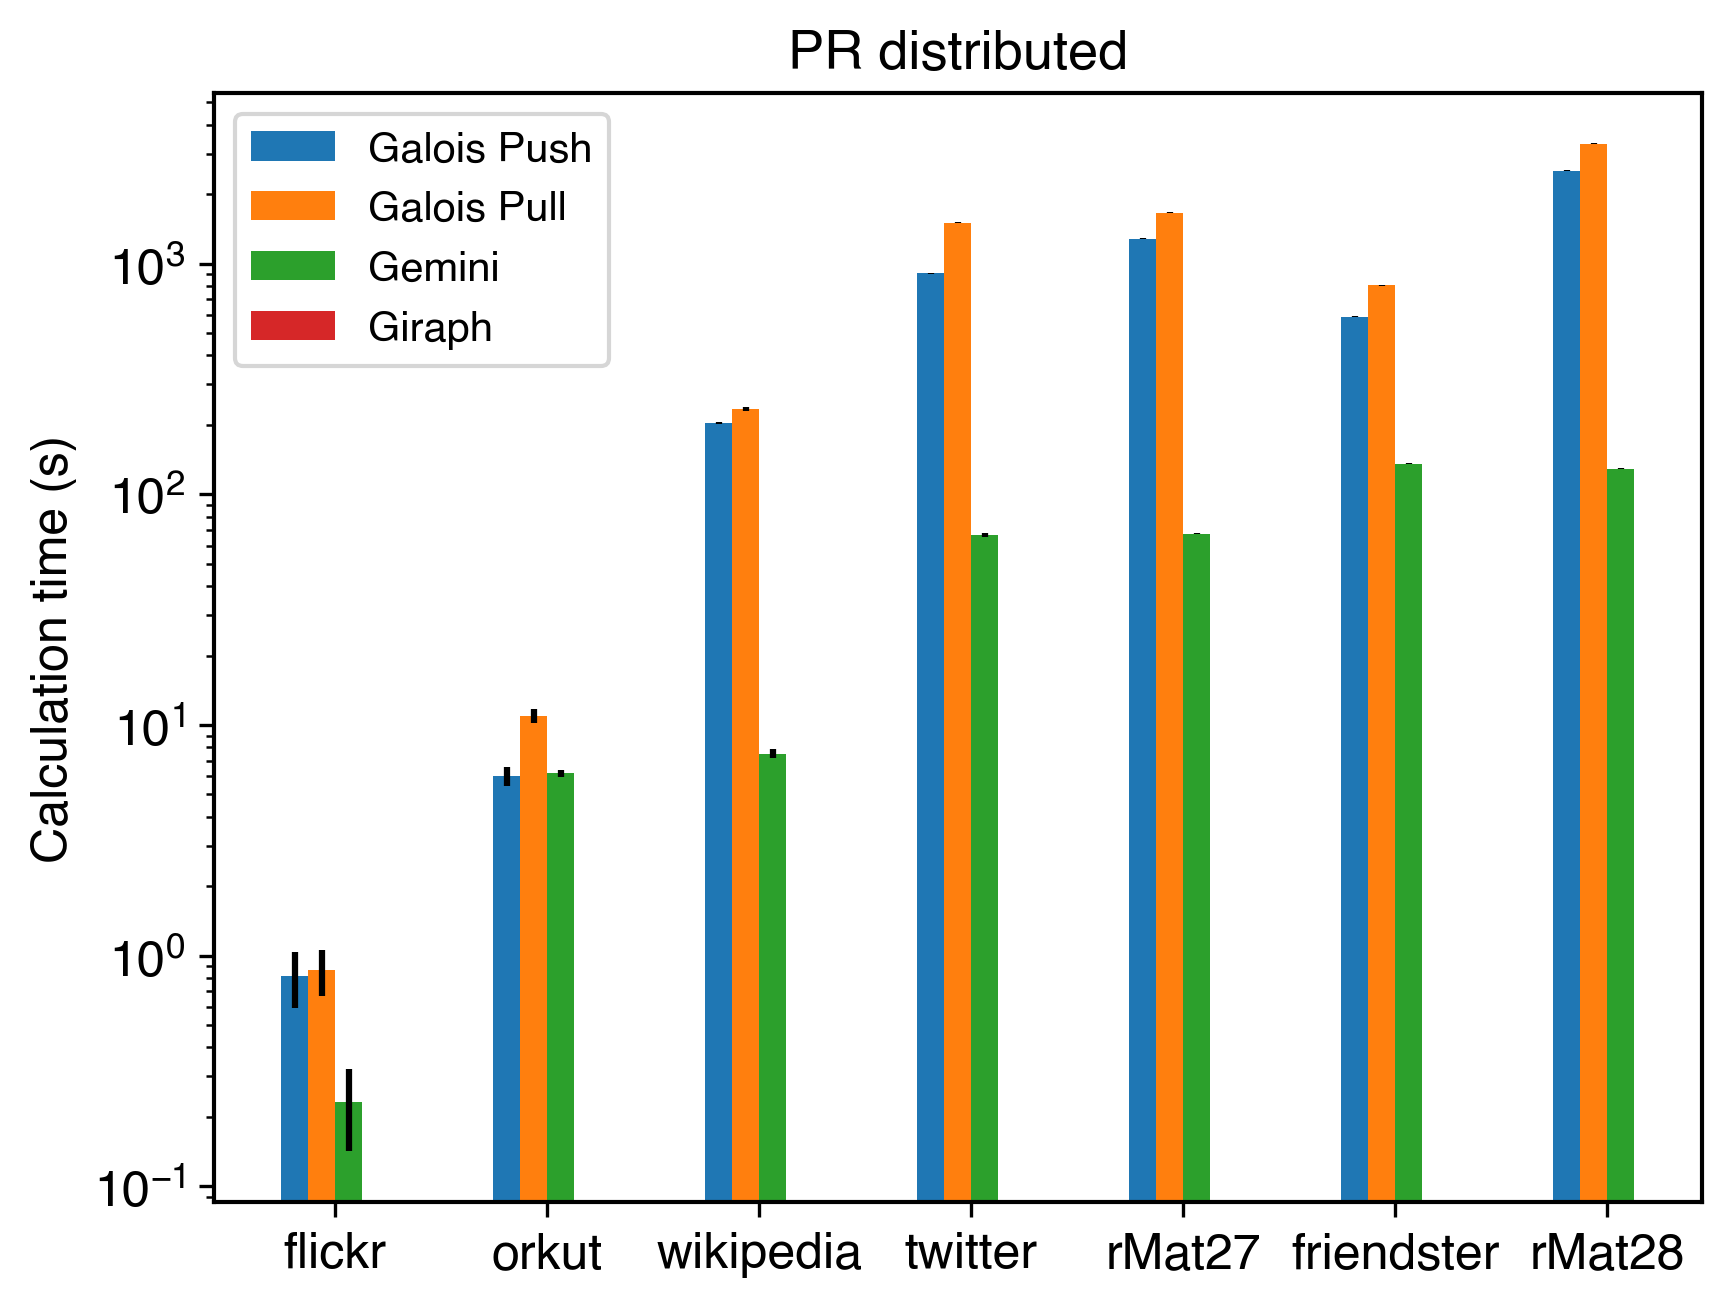
\includegraphics[width=\linewidth]{../../plots/distributedPR_calcTime.png}
		\caption{Calculation time}
		\label{fig:distributedPR_calc}
	\end{subfigure}
	\hfil
	\begin{subfigure}{0.32\textwidth}
		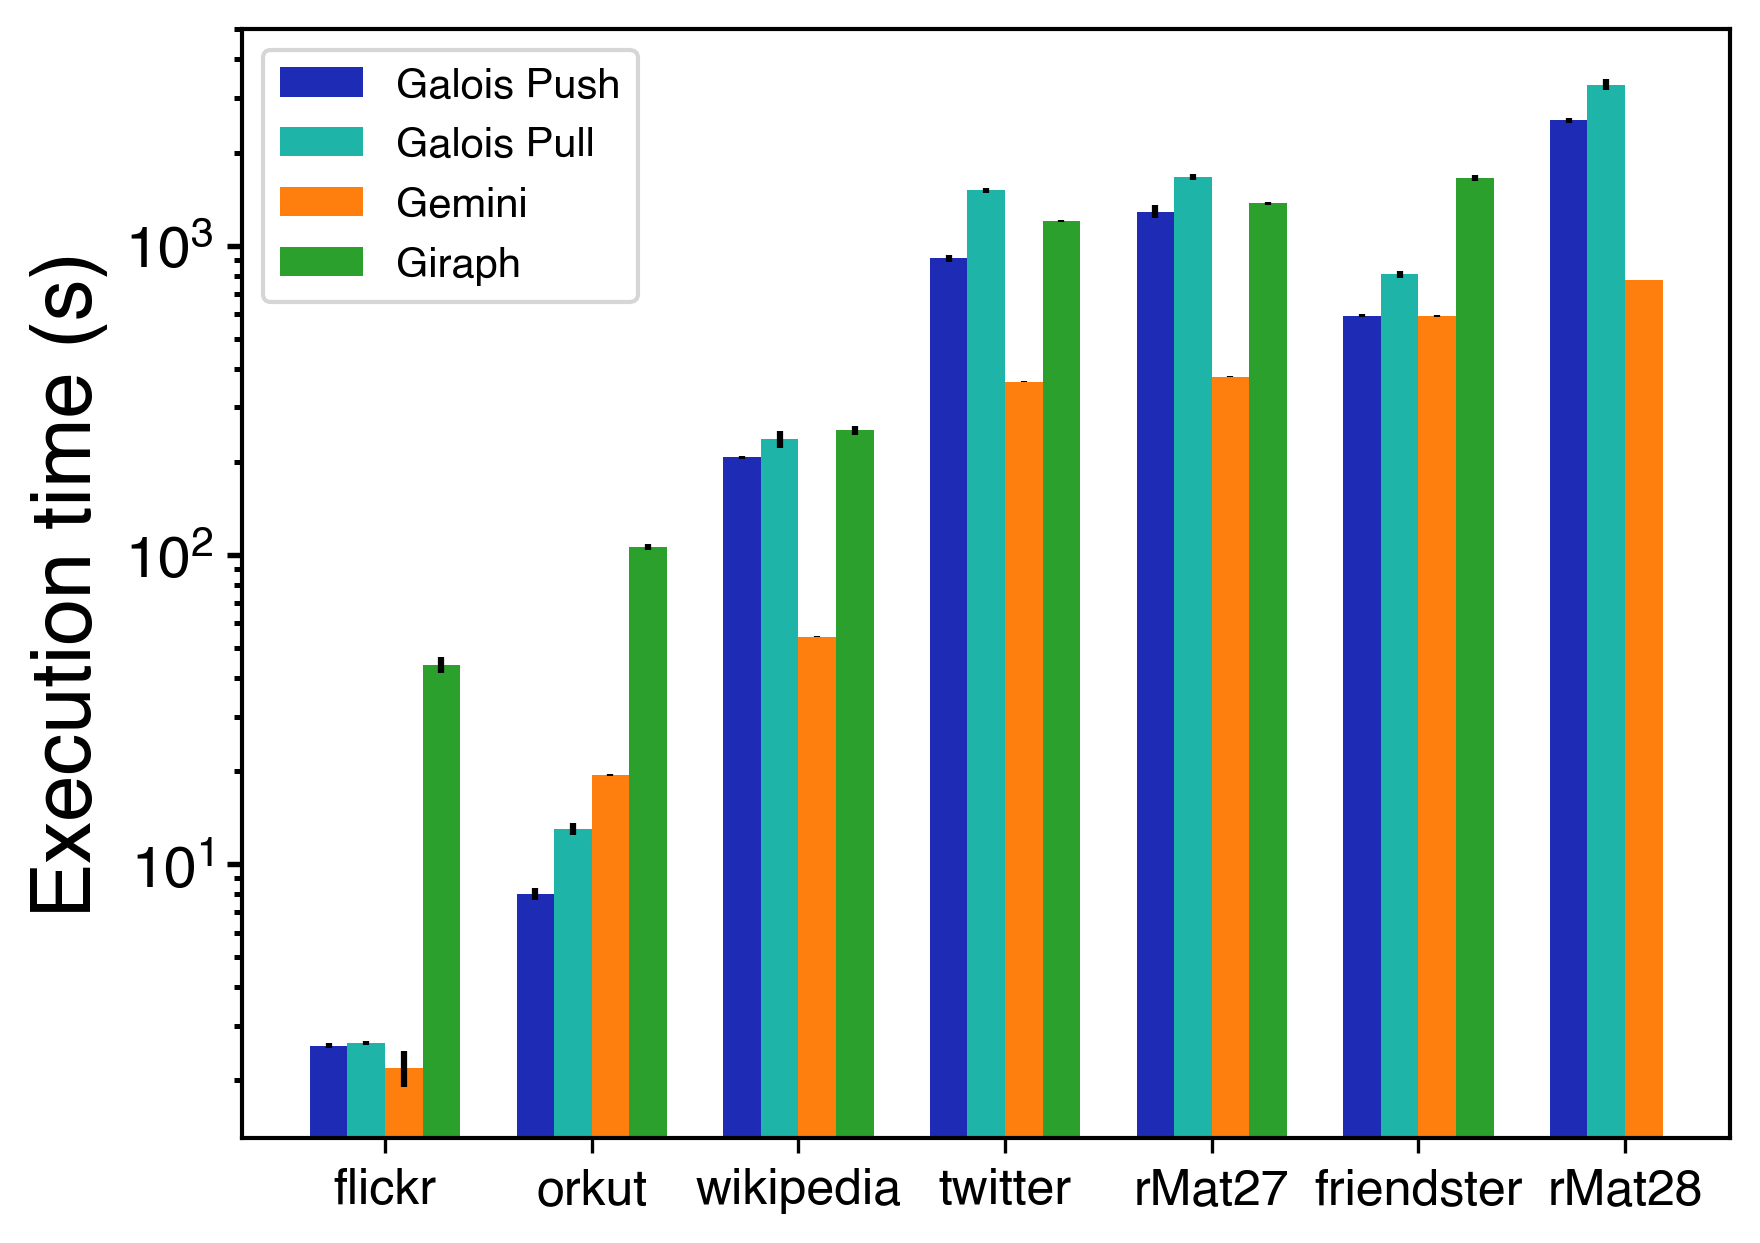
\includegraphics[width=\linewidth]{../../plots/distributedPR_execTime.png}
		\caption{Execution time}
		\label{fig:distributedPR_exec}
	\end{subfigure}
	\hfil
	\begin{subfigure}{0.32\textwidth}
		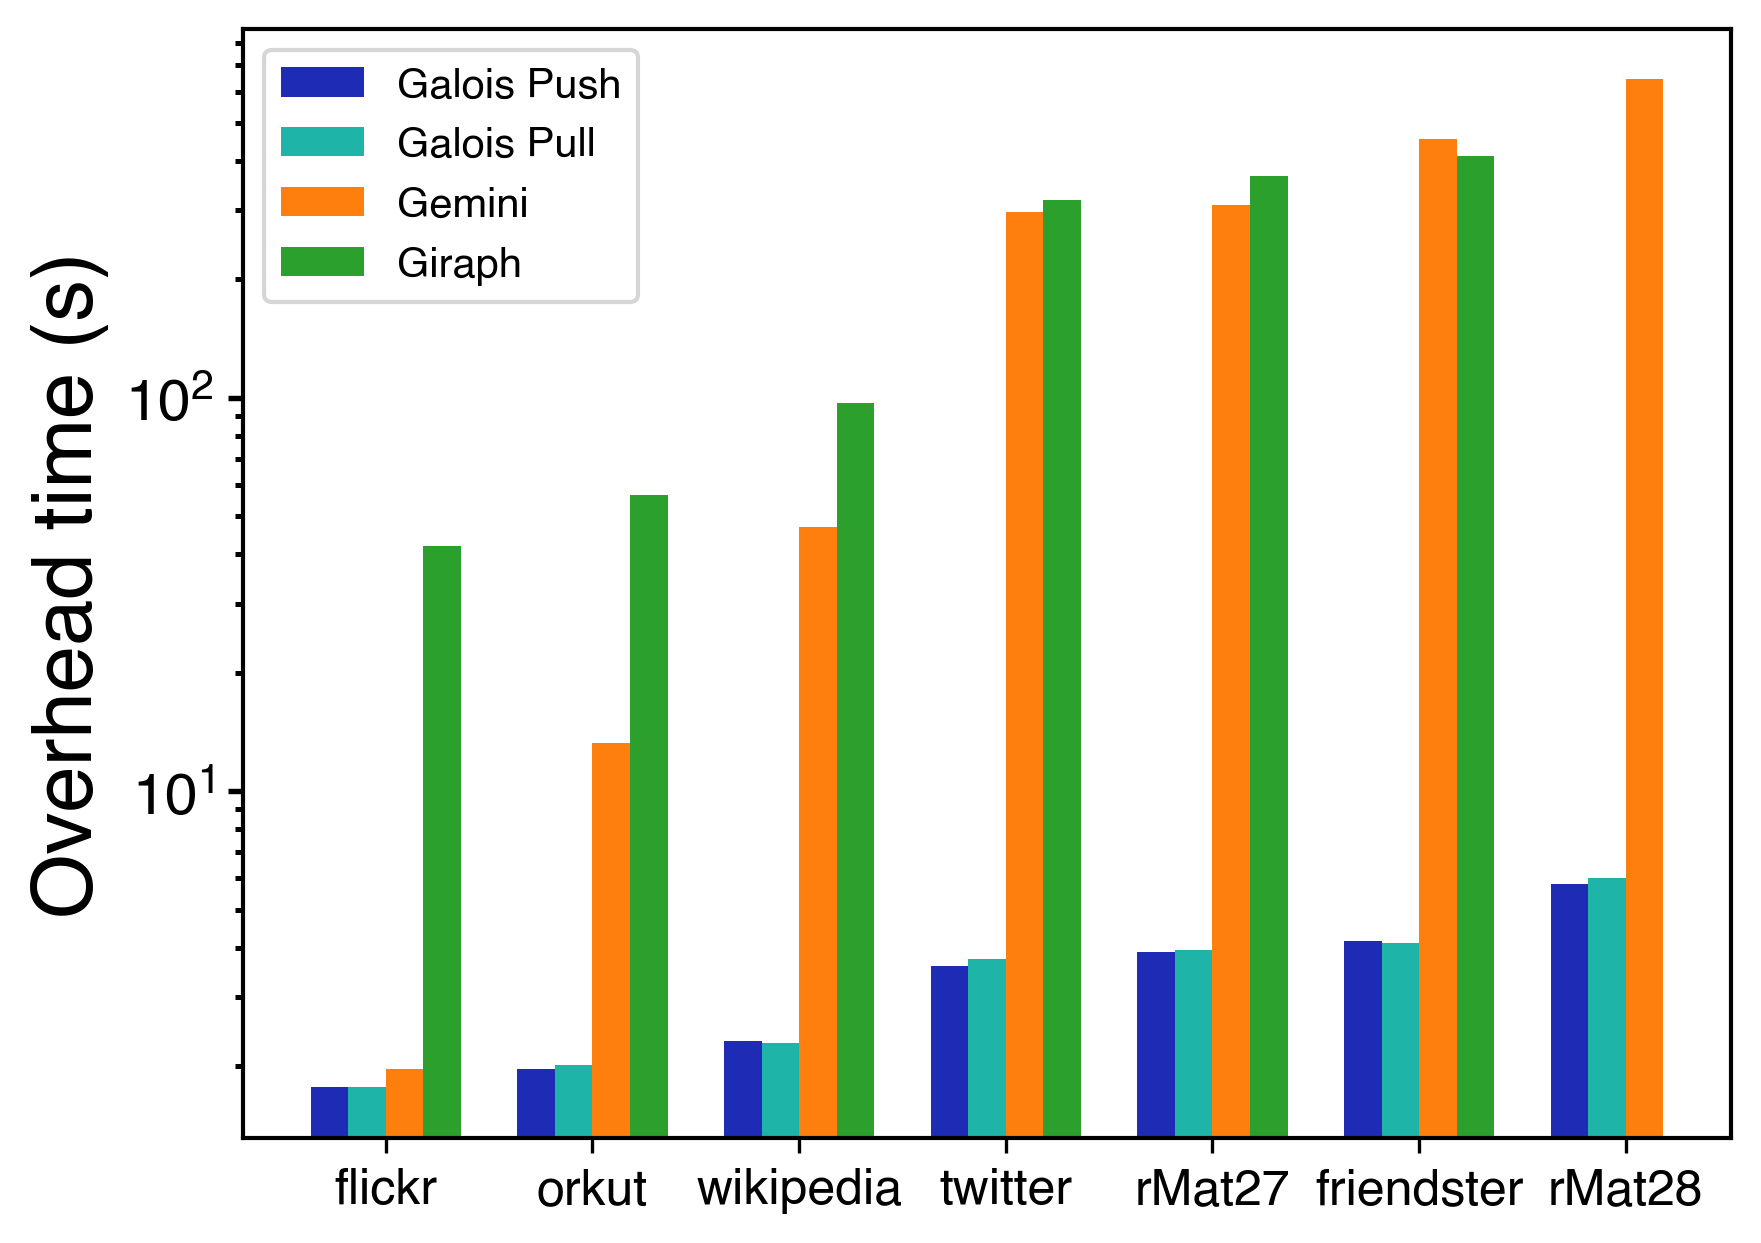
\includegraphics[width=\linewidth]{../../plots/distributedPR_overheadTime.png}
		\caption{Overhead}
		\label{fig:distributedPR_overhead}
	\end{subfigure}
	\hfil
	\caption{Average times for PR on the distributed cluster, black bars represent one standard deviation in our testing}
	\label{fig:distributedPR}
\end{figure*}

Our benchmark results of PageRank on the distributed cluster can be seen in \autoref{fig:distributedPR}.
First of all, Giraph was unable to complete the test on rMat28 because it ran out of memory, thus this result is missing.
When comparing the calculation times in \autoref{fig:distributedPR_calc} to the execution times in \autoref{fig:distributedPR_exec}, we see similar behaviour of all frameworks.
This means that unlike with SSSP or BFS, the calculation times and execution times are similar with respect to the relations of the frameworks to one another.

Gemini has the shortest calculation times on all graphs (cf. \autoref{fig:distributedPR_calc}).
The two Galois implementations are second on flickr, orkut, friendster and rMat28, with Giraph being second on the others.
Generally, the calculation of Galois Push is anywhere from 6\% (flickr) to 46\% (orkut) faster than the Pull counterpart.

This applies to the execution times in almost the same way (cf. \autoref{fig:distributedPR_exec}).
Gemini is the fastest on all graphs except orkut, where both Galois implementations are faster. Galois Pull takes 13s, whereas Gemini requires 19.4s on orkut.
Again, as for the calculation times, Galois is the second fastest framework on flickr, wikipedia, friendster and rMat28.
And Galois Push has smaller execution times than the Pull version because the overhead times for both implementations are similar (cf. \autoref{fig:distributedPR_overhead}).



\subsubsection{Comparison of a Single-Node to the Distributed Cluster}
\begin{table}
	\caption{Execution Times in Seconds on a Single Node vs. 5-Node Distributed Cluster}
	\label{tbl:execTimeComparison}
	\renewcommand{\arraystretch}{1.2}
	\centering
	\begin{tabular}{ccr@{\tabskip 1 \tabcolsep}r
	r@{\tabskip 1 \tabcolsep}r
	r@{\tabskip 1 \tabcolsep}r}
		\toprule
		&&\multicolumn{2}{c}{\bf Galois}&\multicolumn{2}{c}{\bf Gemini}&\multicolumn{2}{c}{\bf Giraph}\\
		\cmidrule{3-4}\cmidrule{5-6}\cmidrule{7-8}
		&\bf Graph&1N&5N&1N&5N&1N&5N\\
		\midrule
		\multirow{7}{0.5ex}{\rotatebox{90}{\bf SSSP}}&flickr & \bf 0.3 & 2.4 & \bf 0.6 & 2.5 & \bf 38.8 & 42.6 \\
		& orkut & \bf 0.8 & 4.2 & \bf 13.9 & 17.3 & 135.9 & \bf 60.4 \\
		& wikipedia & \bf 1.8 & 14.2 & \bf 48.5 & 74.5 & 377.2 & \bf 100.8 \\
		& twitter & \bf 10.8 & 40.0 & \bf 383.0 & 391.1 & - & \bf 349.9 \\
		& rMat27 & \bf 16.0 & 39.0 & 563.5 & \bf 386.0 & - & \bf 565.8 \\
		& friendster & \bf 14.4 & 58.5 & 742.6 & \bf 568.9 & - & \bf 444.0 \\
		& rMat28 & \bf 27.8 & 71.5 & 1236.7 & \bf 792.0 & - & \bf 1180.2 \\
		\midrule
		\multirow{7}{0.5ex}{\rotatebox{90}{\bf BFS}}& flickr & \bf 0.6 & 2.3 & \bf 0.7 & 2.4 & \bf 38.9 & 41.9 \\
		& orkut & \bf 0.9 & 4.0 & \bf 12.5 & 13.8 & 128.2 & \bf 58.1 \\
		& wikipedia & \bf 2.4 & 13.2 & \bf 44.9 & 60.9 & 360.7 & \bf 95.1 \\
		& twitter & \bf 14.2 & 37.9 & 355.0 & \bf 293.2 & - & \bf 322.3 \\
		& rMat27 & \bf 14.6 & 34.4 & 540.8 & \bf 305.3 & - & \bf 539.2 \\
		& friendster & \bf 12.8 & 47.6 & 708.4 & \bf 450.2 & - & \bf 412.3 \\
		& rMat28 & \bf 33.1 & 67.1 & 1178.7 & \bf 634.3 & - & \bf 1135.6 \\
		\midrule
		\multirow{7}{0.5ex}{\rotatebox{90}{\bf PR}}& flickr & \bf 0.3\txtdagger & 2.6 & \bf 0.7 & 2.2 & 45.6 & \bf 44.1 \\
		& orkut & \bf 0.7\txtdagger & 8.0 & \bf 13.1 & 19.4 & 561.3 & \bf 106.2 \\
		& wikipedia & \bf 1.7\txtdagger & 206.5 & \bf 44.4 & 54.4 & 1501.3 & \bf 252.6 \\
		& twitter & \bf 8.7\txtdagger & 910.9 & \bf 359.9 & 363.5 & - & \bf 1200.2 \\
		& rMat27 & \bf 19.2\txtdagger & 1287.4 & 536.3 & \bf 376.3 & - & \bf 1369.5 \\
		& friendster & \bf 20.4\txtdagger & 593.3 & 716.5 & \bf 591.1 & - & \bf 1655.0 \\
		& rMat28 & \bf 46.0\txtdagger & 2540.2 & 1188.5 & \bf 774.2 & - & - \\
		\bottomrule
		\multicolumn{8}{l}{(\txtdagger) Results of Galois Pull shown.}
	\end{tabular}
\end{table}
Until now, we have only compared the frameworks with each other, under the same setup circumstances. Hence, a comparison of the same framework, in single-node versus distributed setup is the content of this section.
Of course only frameworks that were tested in both setups are shown.
We focus primarily on the results of the execution times, the data can be seen in \autoref{tbl:execTimeComparison}. We show the results of Galois Push for the 5-node cluster in the table, since it is faster than Pull.

There are some, rather large differences in the execution times of each framework. Galois is consistently faster on a single computation node compared to the distributed setup. 
On both SSSP and BFS, the margin between the two setups is already noticeable. The distributed scenario requires from 2$\times$ (BFS, rMat28) to 7.8$\times$ (SSSP, wikipedia) the execution time of single-node Galois.
For PR however, the difference is multiple orders of magnitude large. Distributed Galois requires from 8.6$\times$ to 121$\times$ more time than single-node Galois. 

Gemini's distributed calculation only requires more time on the smaller graphs (i.e. flickr to wikipedia). There, the distributed scenario is anywhere from 1.1$\times$ (BFS, orkut) to 4.2$\times$ (SSSP, flickr) slower.
Twitter is the tipping point for Gemini's SSSP and PR algorithm. Here, execution times on the single-node and distributed cluster are within 2\% of each other. For BFS, the tipping point is anywhere between twitter and rMat27.
Above that, i.e. on the larger graphs, the added computation power can be leveraged to overcome the synchronization overhead of the distributed scenario. Hence, on those graphs single-node Gemini becomes up to 1.8$\times$ (BFS, rMat28) slower than the distributed version.
This relation is very dependent on the graph size. The smaller the graph, the faster single-node Gemini is in comparison. Analogously, the larger the graph, the larger the gap becomes, in favour of the distributed version.

A very similiar behaviour can be observed for Giraph, but the relation tips in favour of the distributed version much sooner. Giraph already uses the distributed cluster efficiently on the smaller graphs as well.
On flickr, the execution times of single-node vs distributed Giraph are already within 9\% of each other.
On the larger graphs, the differences quickly increase, again in favour of the distributed scenario. Giraph's single-node version runs up to 5.9$\times$ (PR, wikipedia) slower than the distributed version.
Keep in mind, that only a comparison between the three smallest graphs can be made here.

%!TEX root=../../main.tex




\subsection{Galois speedup}
\label{sec:galois_speedup}
Analyzing the calculation time speedups for Galois, we can compare how or if the different algorithms benefit from increasing thread numbers.


\begin{figure*}
	\hfil
	\begin{subfigure}{0.32\textwidth}
		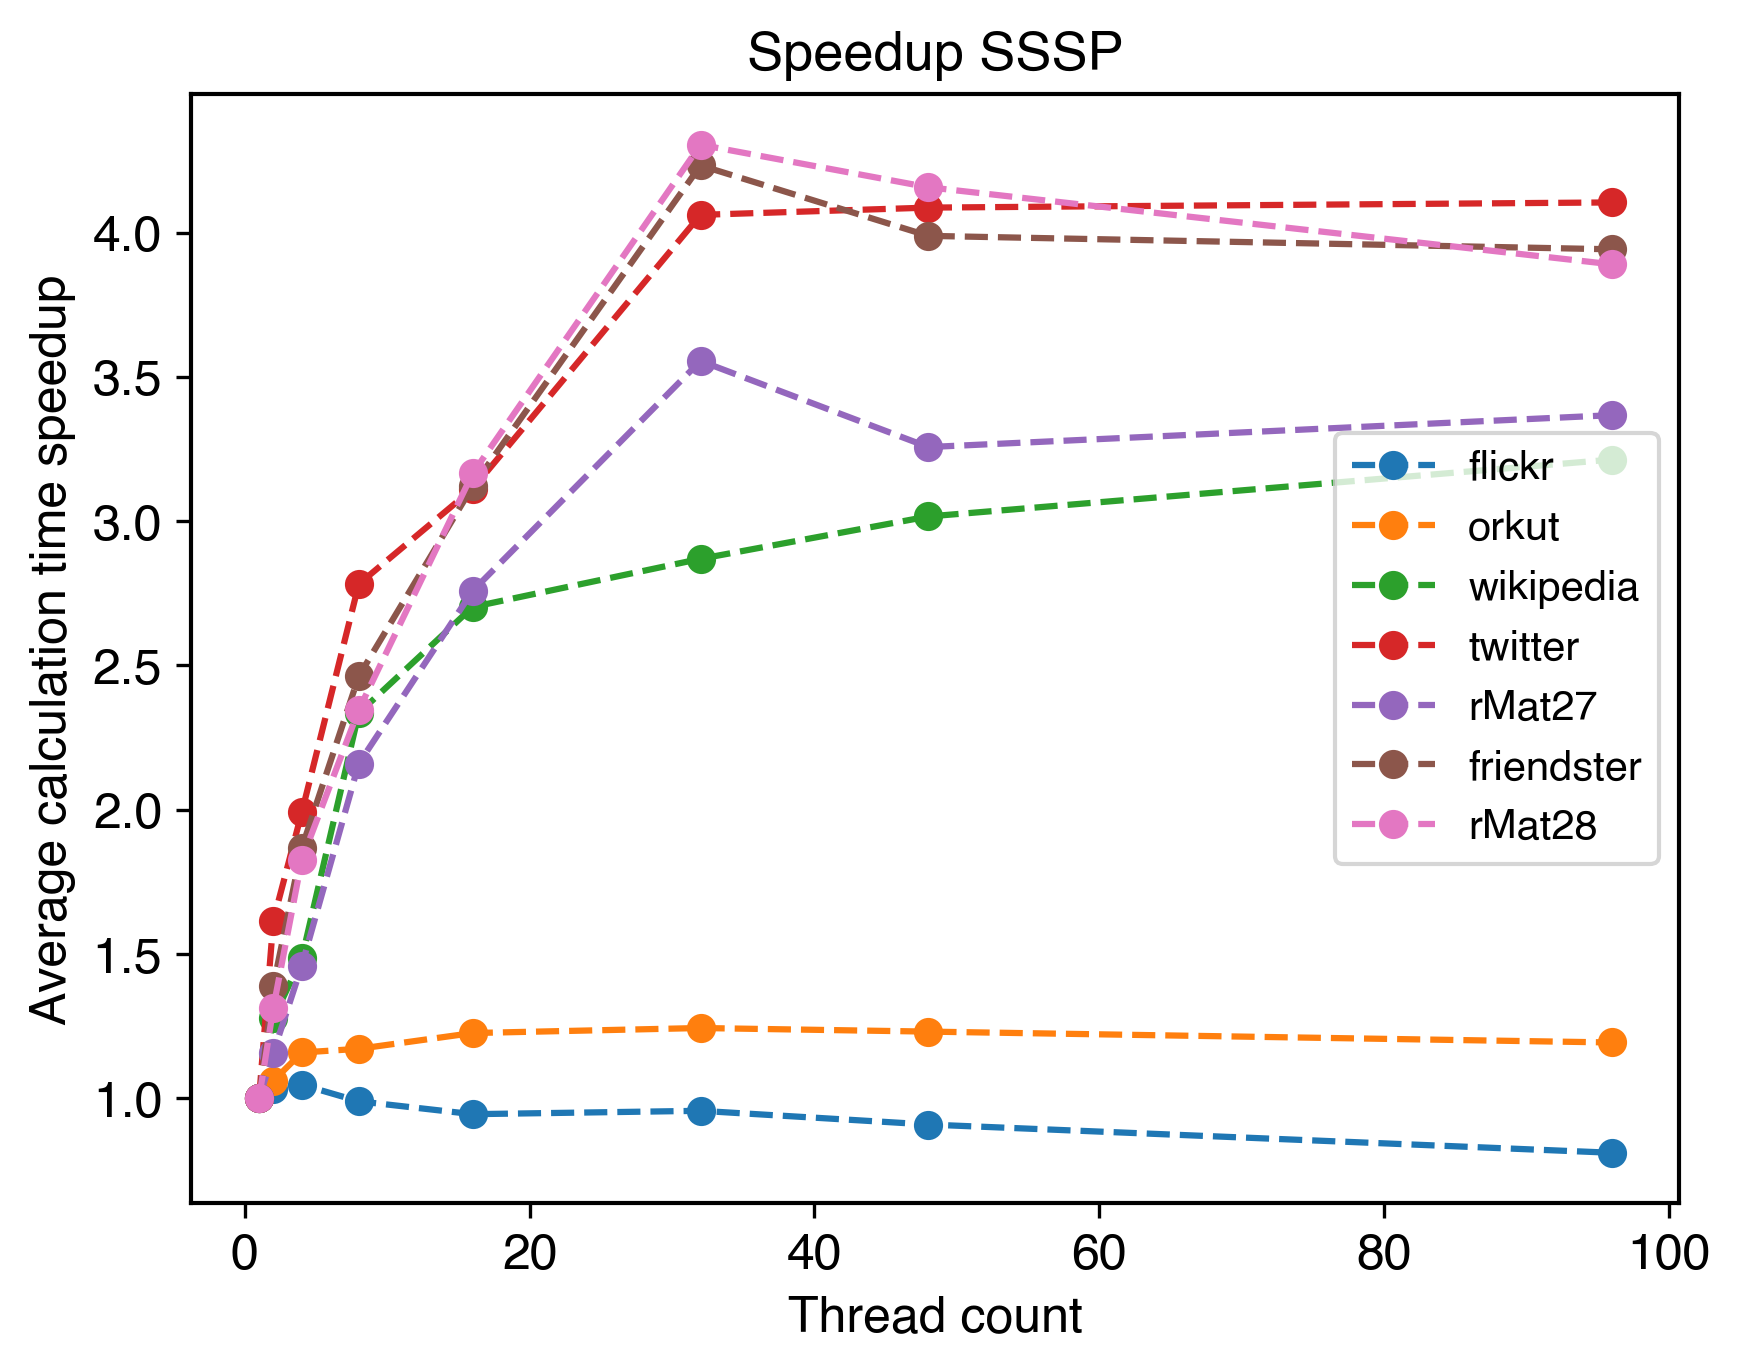
\includegraphics[width=\linewidth]{../../plots/singleNodeSSSPGaloisThreads.png}
		\caption{Calculation time speedup with increasing thread count for Galois Single-source Shortest-paths}
		\label{fig:galoisSpeedupSSSP}
	\end{subfigure}
	\hfil
	\begin{subfigure}{0.32\textwidth}
		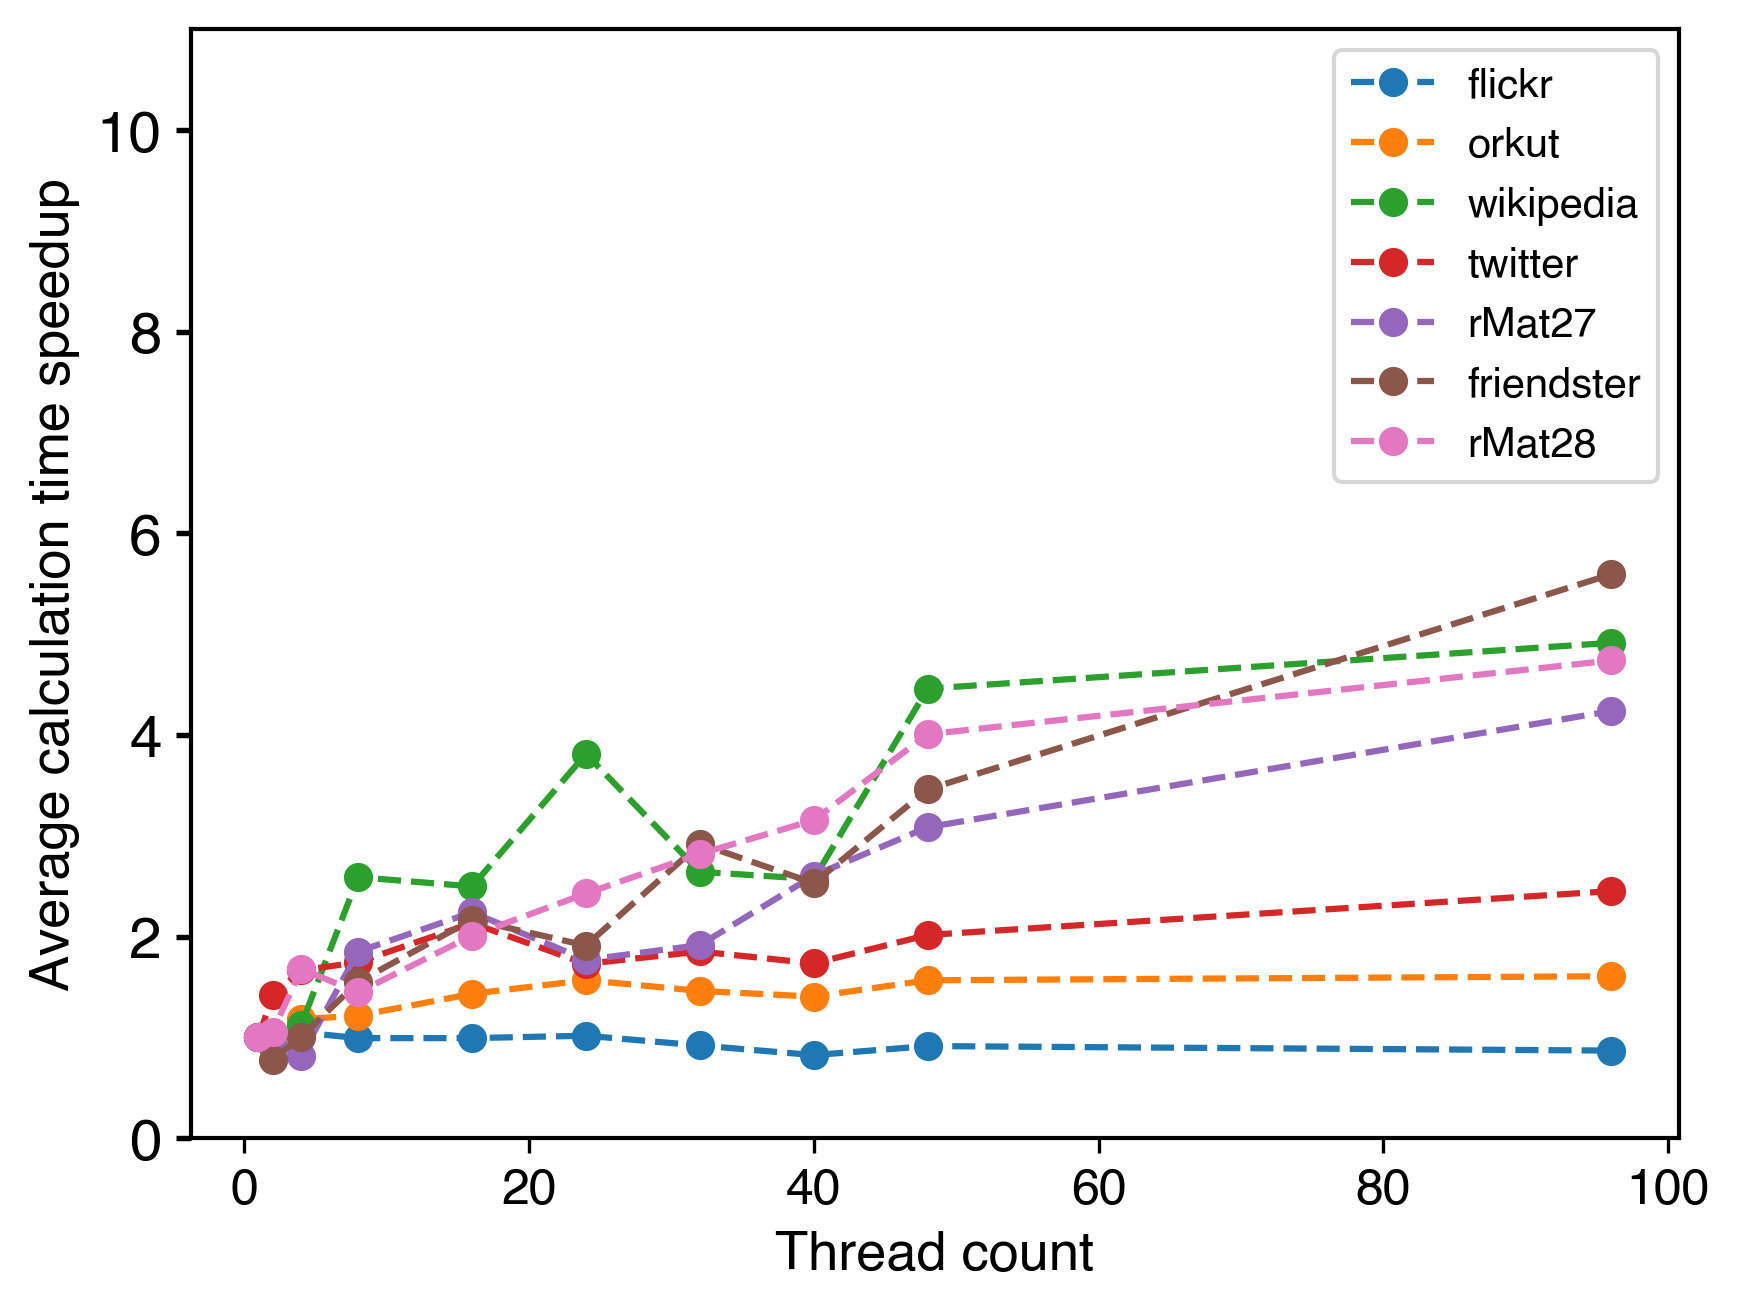
\includegraphics[width=\linewidth]{../../plots/singleNodeBFSGaloisThreads.png}
		\caption{Calculation time speedup with increasing thread count for Galois Breadth-first search}
		\label{fig:galoisSpeedupBFS}
	\end{subfigure}
	\hfil
\end{figure*}



\subsubsection{Single-source Shortest-path}

Starting with SSSP, we see an algorithm that benefits from many available threads in \autoref{fig:galoisSpeedupSSSP}.
For all larger graphs, speedup is in most cases very close to optimal up to about 8 threads.
Twitter has the best speedup overall. It is 2.6$\times$ with 2 threads compared to one, 4$\times$ with 4, 7.7$\times$ with 8 and 9.7$\times$ using 16 threads.
Behaviour on friendster is similarly good. Here speedup is 1.9$\times$ at 2 threads compared to one, 3.5$\times$ at 4, 6.1$\times$ at 8 threads and 9.7$\times$ at 16 threads.
Anything above 16 threads however no longer helps decrease the computation time significantly on any graph. Speedup above 16 threads is always less than double the speedup of 16 threads. The maximum measured speedups are 10$\times$ (96 threads) for wikipedia, 17$\times$ (96 threads) for twitter, 11$\times$ (96 threads) for rMat27, 16$\times$ (48 threads) for friendster and 19$\times$ (40 threads) for rMat28.
In some cases increasing thread counts even prolongues calculation time. For example calculation on rMat28 is actually slower with 48 or 96 threads compared to 40 threads. For 40 threads, the speedup is nearly 19$\times$, on 48 threads 17$\times$ and with 96 threads only 15$\times$ compared to one thread.

Small graphs, i.e. flickr and orkut neither benefit from more threads nor is the performance significantly held up by synchronization overhead.
Performance on flickr can not be sped up at all, with speedup on flickr being very close to 1 for 1 to 8 threads and between 0.7$\times$ to 0.9$\times$ from 16 to 96 threads.
Orkut reaches maximum speedup of 1.6$\times$ at 16 threads. However on orkut, the speedup is always greater or equal to 1.


\subsubsection{Breadth-first search}


For our speedup results on BFS, \autoref{fig:galoisSpeedupBFS} shows the calculation time speedup of Galois' BFS.
On all graphs, the speedup never exceeds 6$\times$ even when using 96 threads.
For the smaller graphs (flickr, orkut), we have the same behaviour as on SSSP. Speedup is close to 1 in all cases, with orkut reaching a maximum speedup of 1.6$\times$ at 24 threads.
On the larger graphs, speedup is possible but only to a very small degree.
Wikipedia has a maximum speedup of 4.9$\times$ at 96 threads, for twitter it is 2.5$\times$ at 96 threads and 5.6$\times$ on friendster. The two synthetic data sets reach speedups of 4.2$\times$ and 4.7$\times$ for rMat27 and rMat28 on 96 threads.


\subsubsection{PageRank}
We want to first take a look at the results for PageRank in Pull mode, seen in \autoref{fig:galoisSpeedupPRPull}. This is a perfect example for an algorithm that does not benefit from multithreaded computation.
Computation is hardly sped up on any graph other than flicker, where the reached maximum is 64\%. This maximum is reached at two threads, with speedup steadily declining above that.
The rMat28 is the only other graph of one could say computation was sped up at large thread counts. Here we reached a maximum speedup of 31\%\ at 96 threads.
All 5 other graphs only reach a speedup greater or equal to 1 in just one or two cases and if so only by a small margin.
Computation on Orkut and Twitter reaches a speedup maximum of 12\%\ and 5\%\ at 4 threads, while being less or equal to 1 in all other cases.
The wikipedia graph is never sped up.
Friendster and rMat27 can be sped up by 6.5\%\ or 10\%\ respectively on 8 threads.

Speedup results on PageRank show odd behaviour in the Galois implementation.
There is a significant performance loss on 4, 24 and 40 threads that is far from the expected behaviour. This is most visible for the Push variant seen in \autoref{fig:galoisSpeedupPRPush}, we validated the shown results two times.
Especially, the speedup for 24 threads is (by interpolating between 16 and 32 threads) expected to be anywhere between 25\% and 94\%.
Actually however, the system does not reach a speedup of more than 4\%\ on any graph, with only rMat27 actually reaching a value greater than 1.
On all other graphs, using 24 threads is anywhere from 3\% (flickr) to 9\%\ (wikipedia) slower than using just one thread.

Similar yet less pronounced behaviour is oberservable for Pull in \autoref{fig:galoisSpeedupPRPull}.
Here especially the values for 24 and 40 threads show a loss in performance.
It is most visible on the values for twitter and friendster, where both values drop significantly compared to the neighbouring 32 and 48 thread results.

\begin{figure*}
	\hfil
	\begin{subfigure}{0.32\textwidth}
		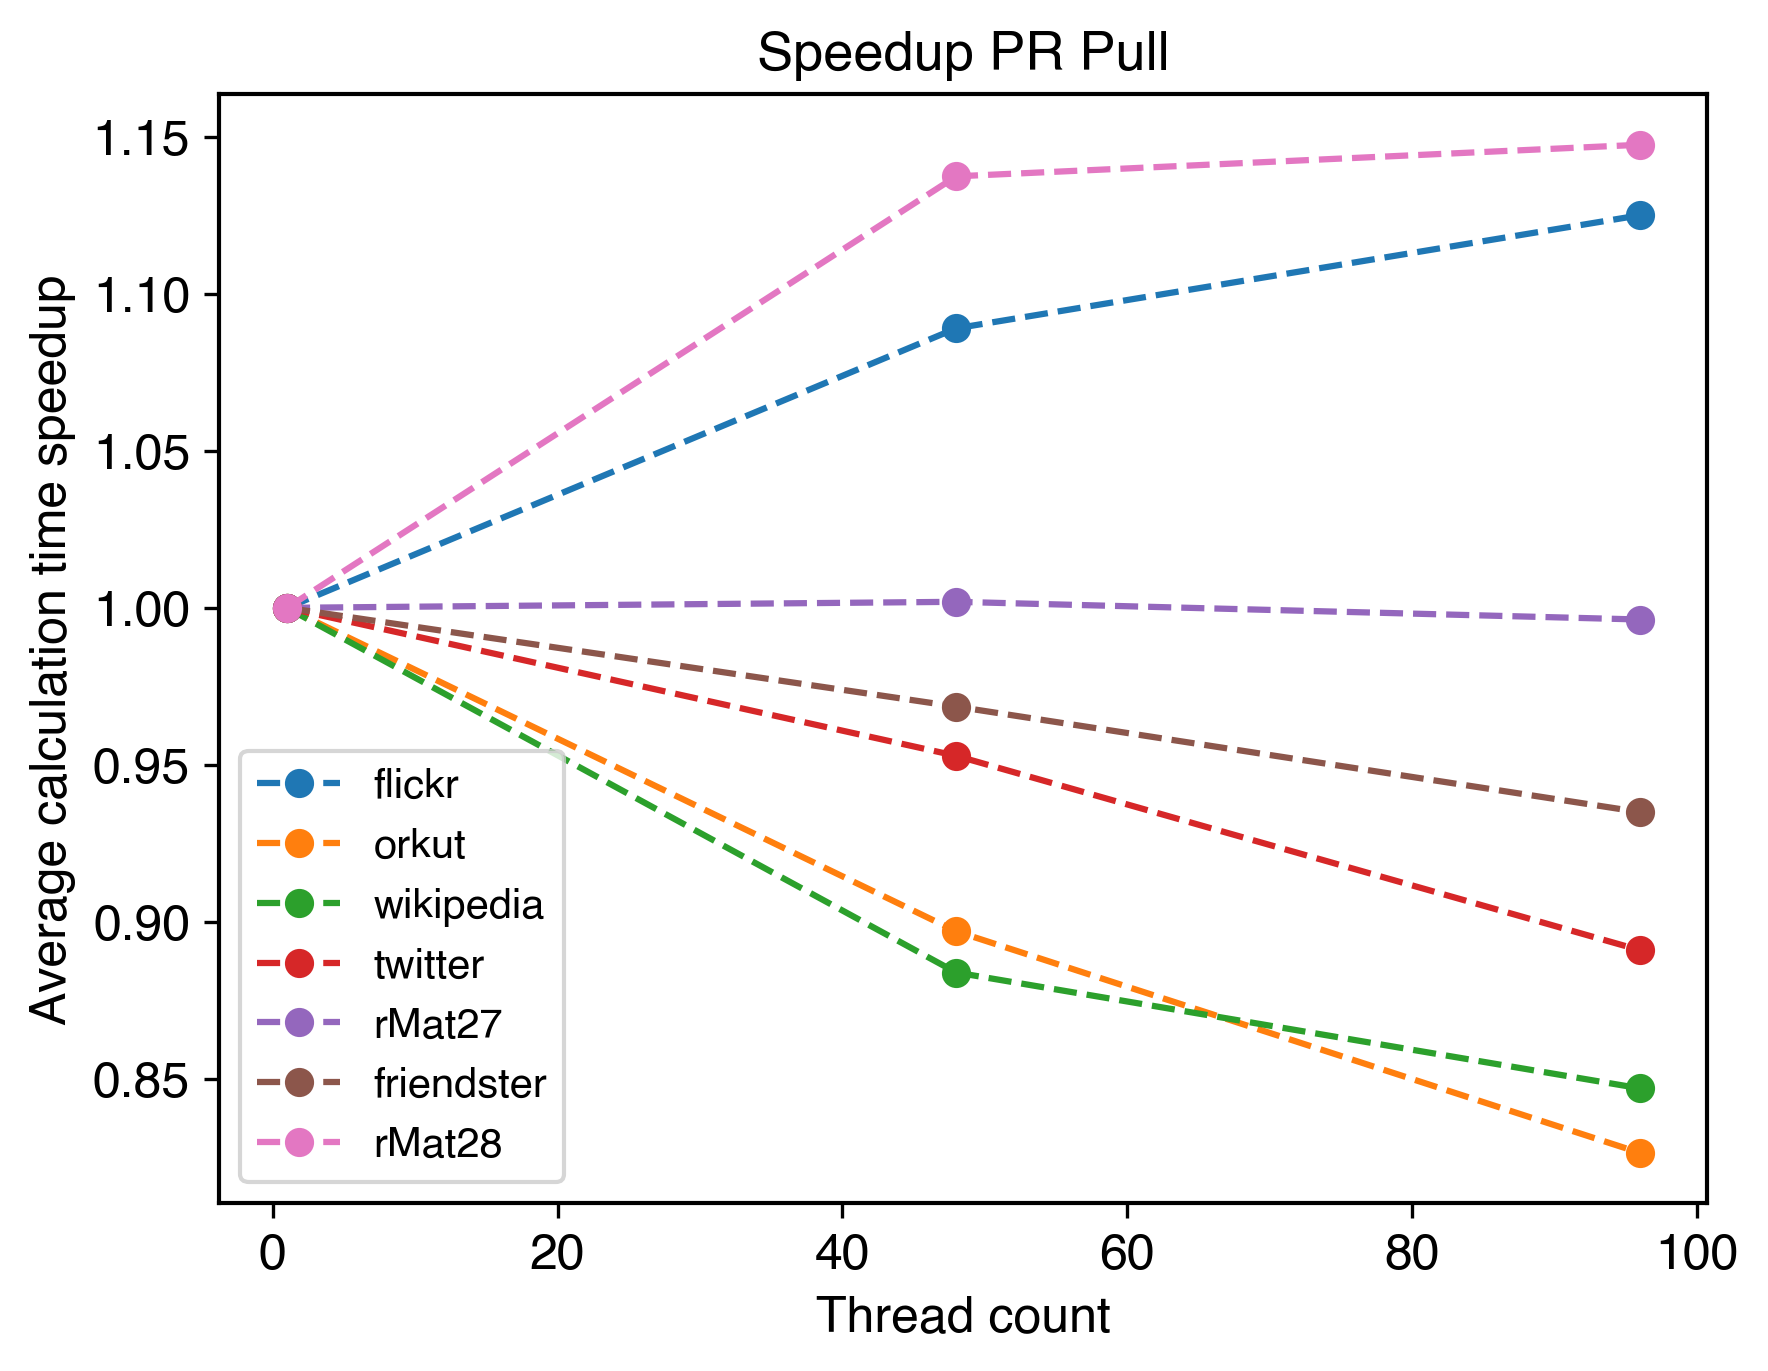
\includegraphics[width=\linewidth]{../../plots/singleNodePRPullGaloisThreads.png}
		\caption{PageRank Pull}
		\label{fig:galoisSpeedupPRPull}
	\end{subfigure}
	\hfil
	\begin{subfigure}{0.32\textwidth}
		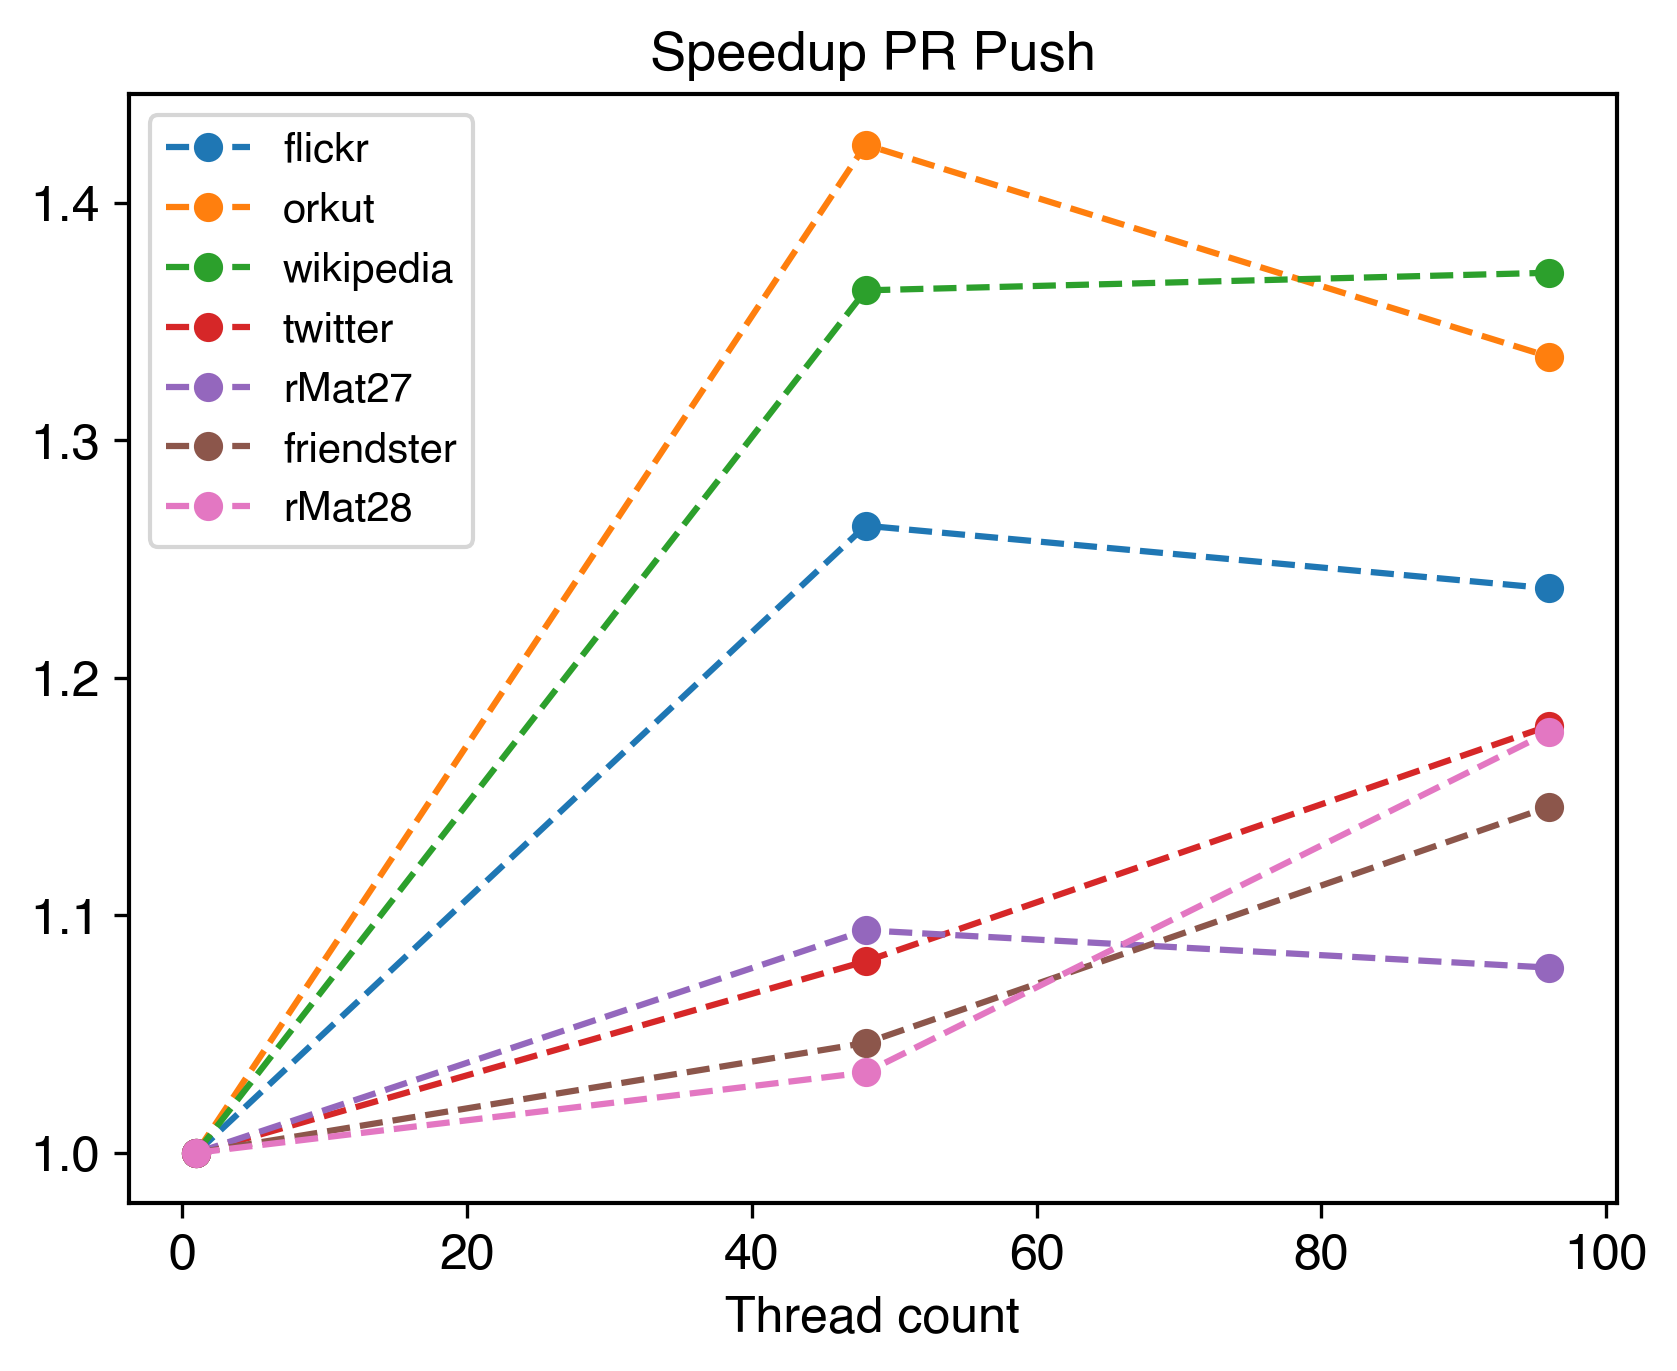
\includegraphics[width=\linewidth]{../../plots/singleNodePRPushGaloisThreads.png}
		\caption{PageRank Push}
		\label{fig:galoisSpeedupPRPush}
	\end{subfigure}
	\hfil
	\caption{Calculation time speedup with increasing thread count for Galois PageRank Push and Pull algorithms.}
\end{figure*}


\section{Hugepages}
\todo{Section}
\begin{figure}
	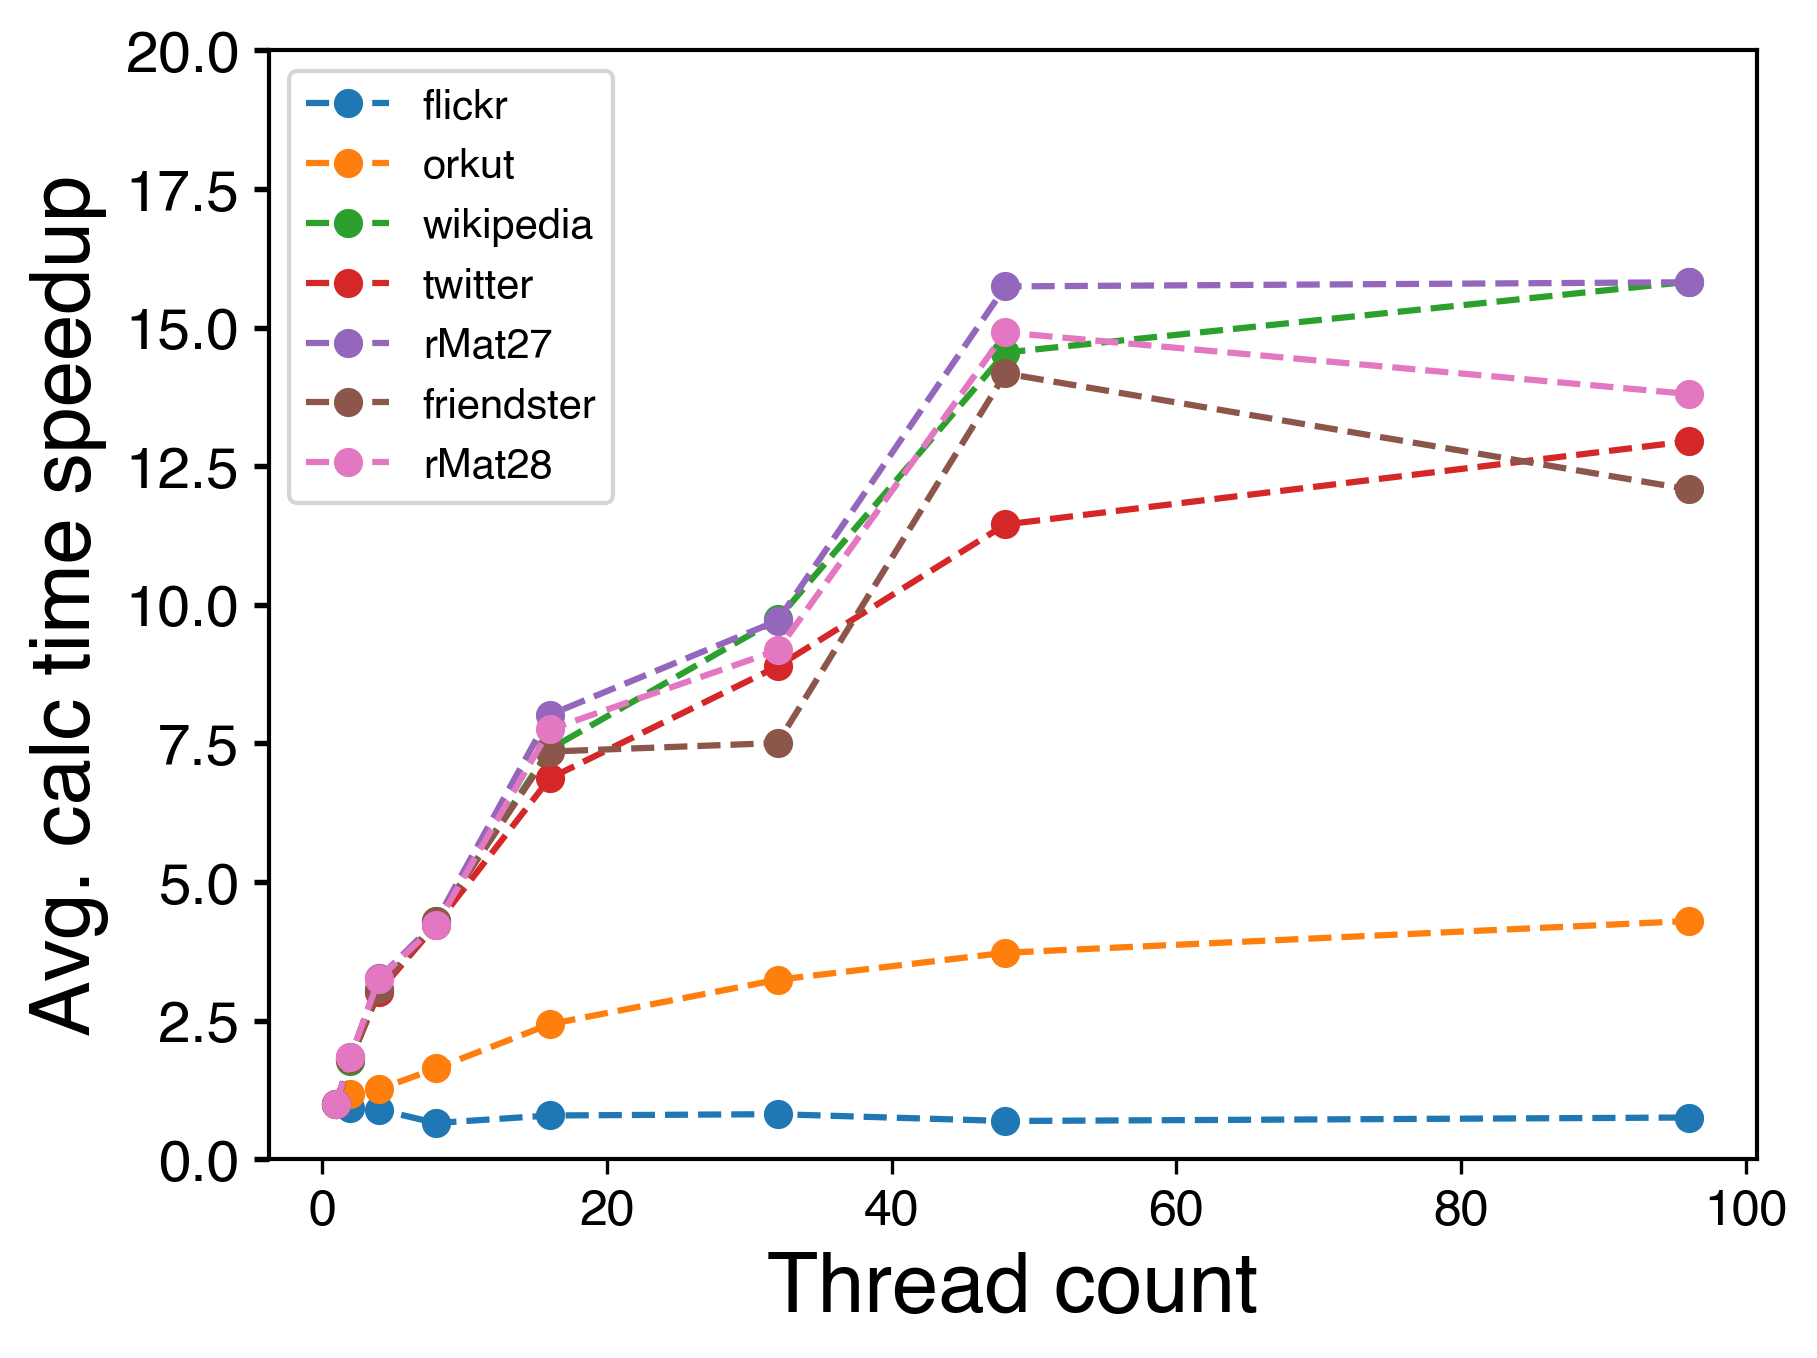
\includegraphics[width=\linewidth]{../../plots/singleNodeSSSPGaloisHPThreads.png}
	\caption{Calculation time speedup with increasing thread count for Galois Single-source Shortest-paths with Hugepages}
	\label{fig:galoisHPSpeedupSSSP}
\end{figure}

\begin{figure}
	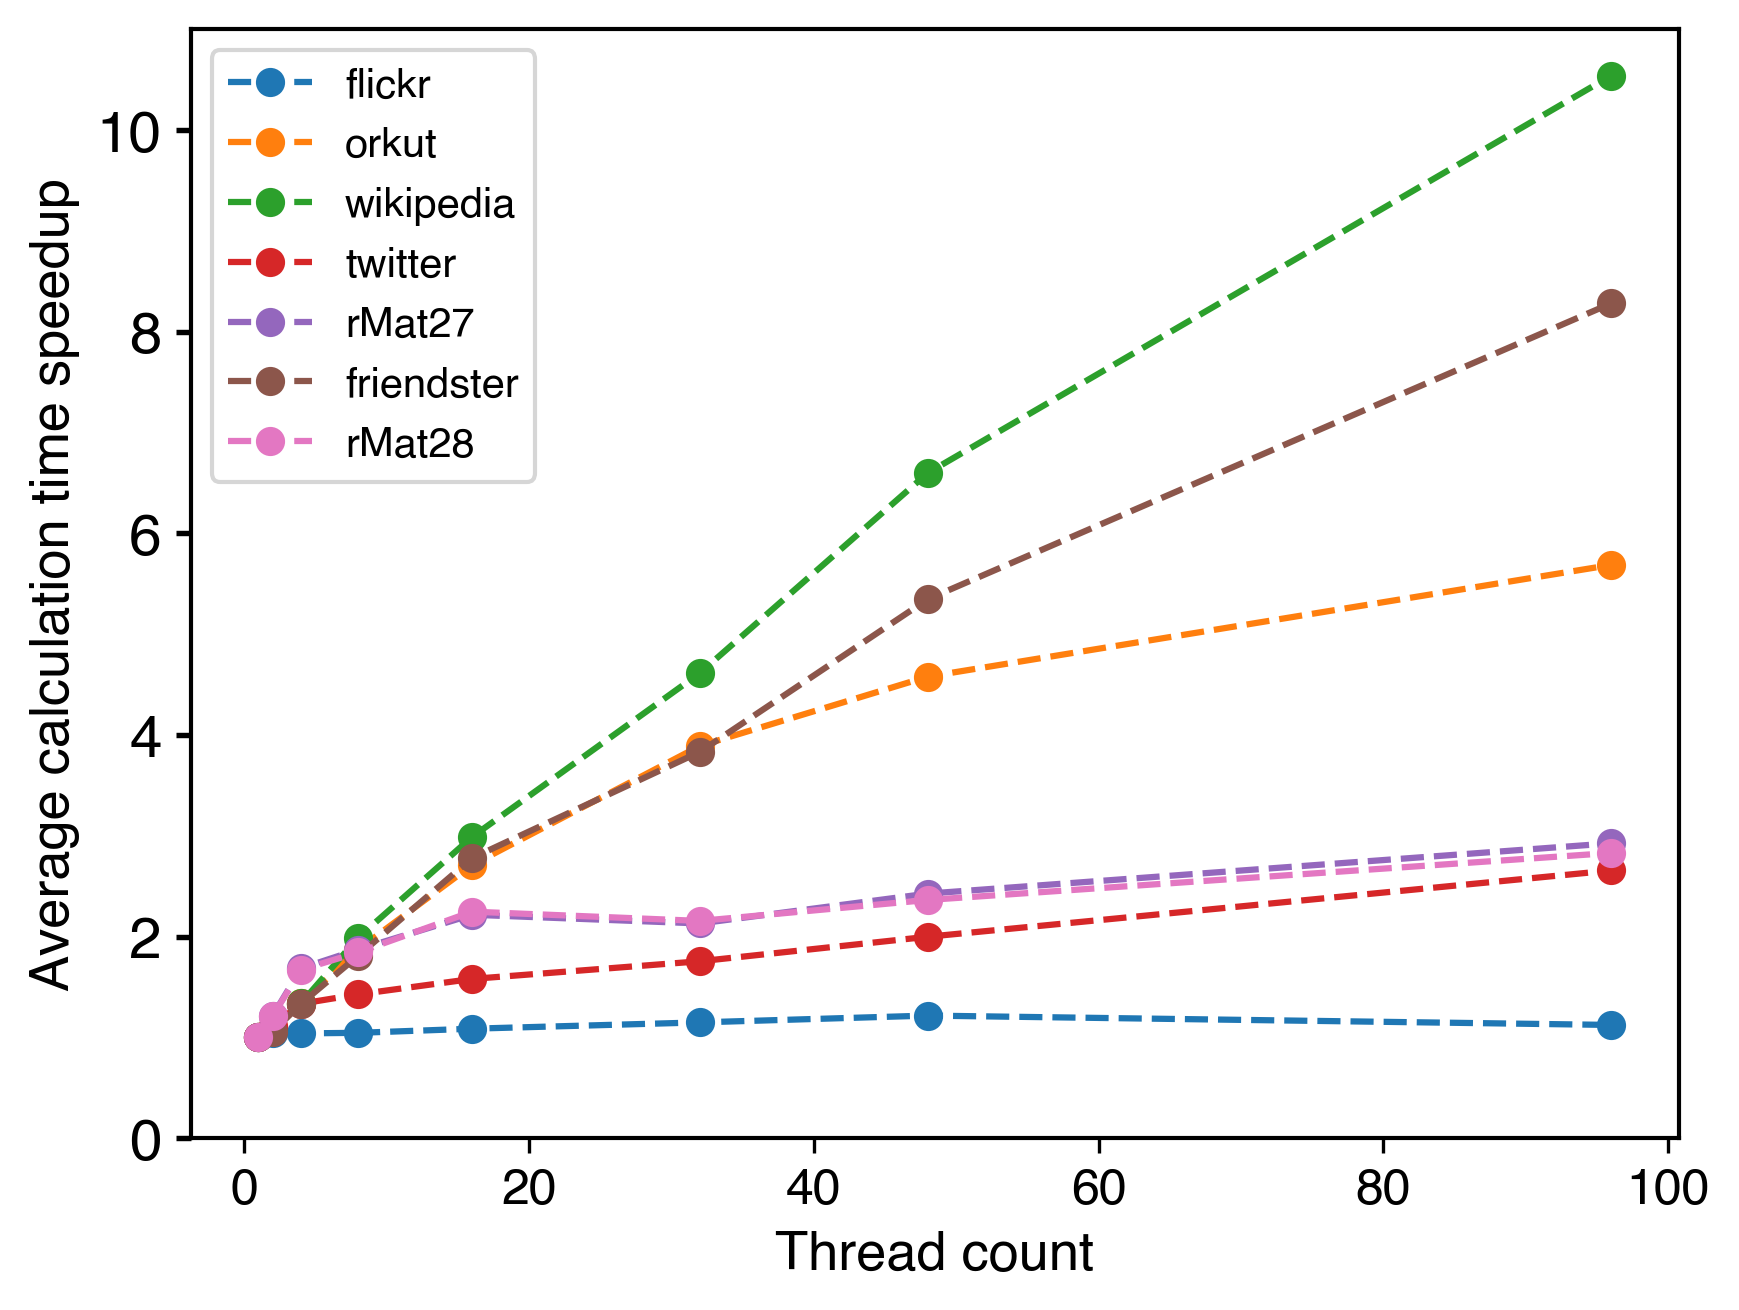
\includegraphics[width=\linewidth]{../../plots/singleNodeBFSGaloisHPThreads.png}
	\caption{Calculation time speedup with increasing thread count for Galois Breadth-first search with Hugepages}
	\label{fig:galoisHPSpeedupBFS}
\end{figure}

\begin{figure}
	\begin{subfigure}{\columnwidth}
		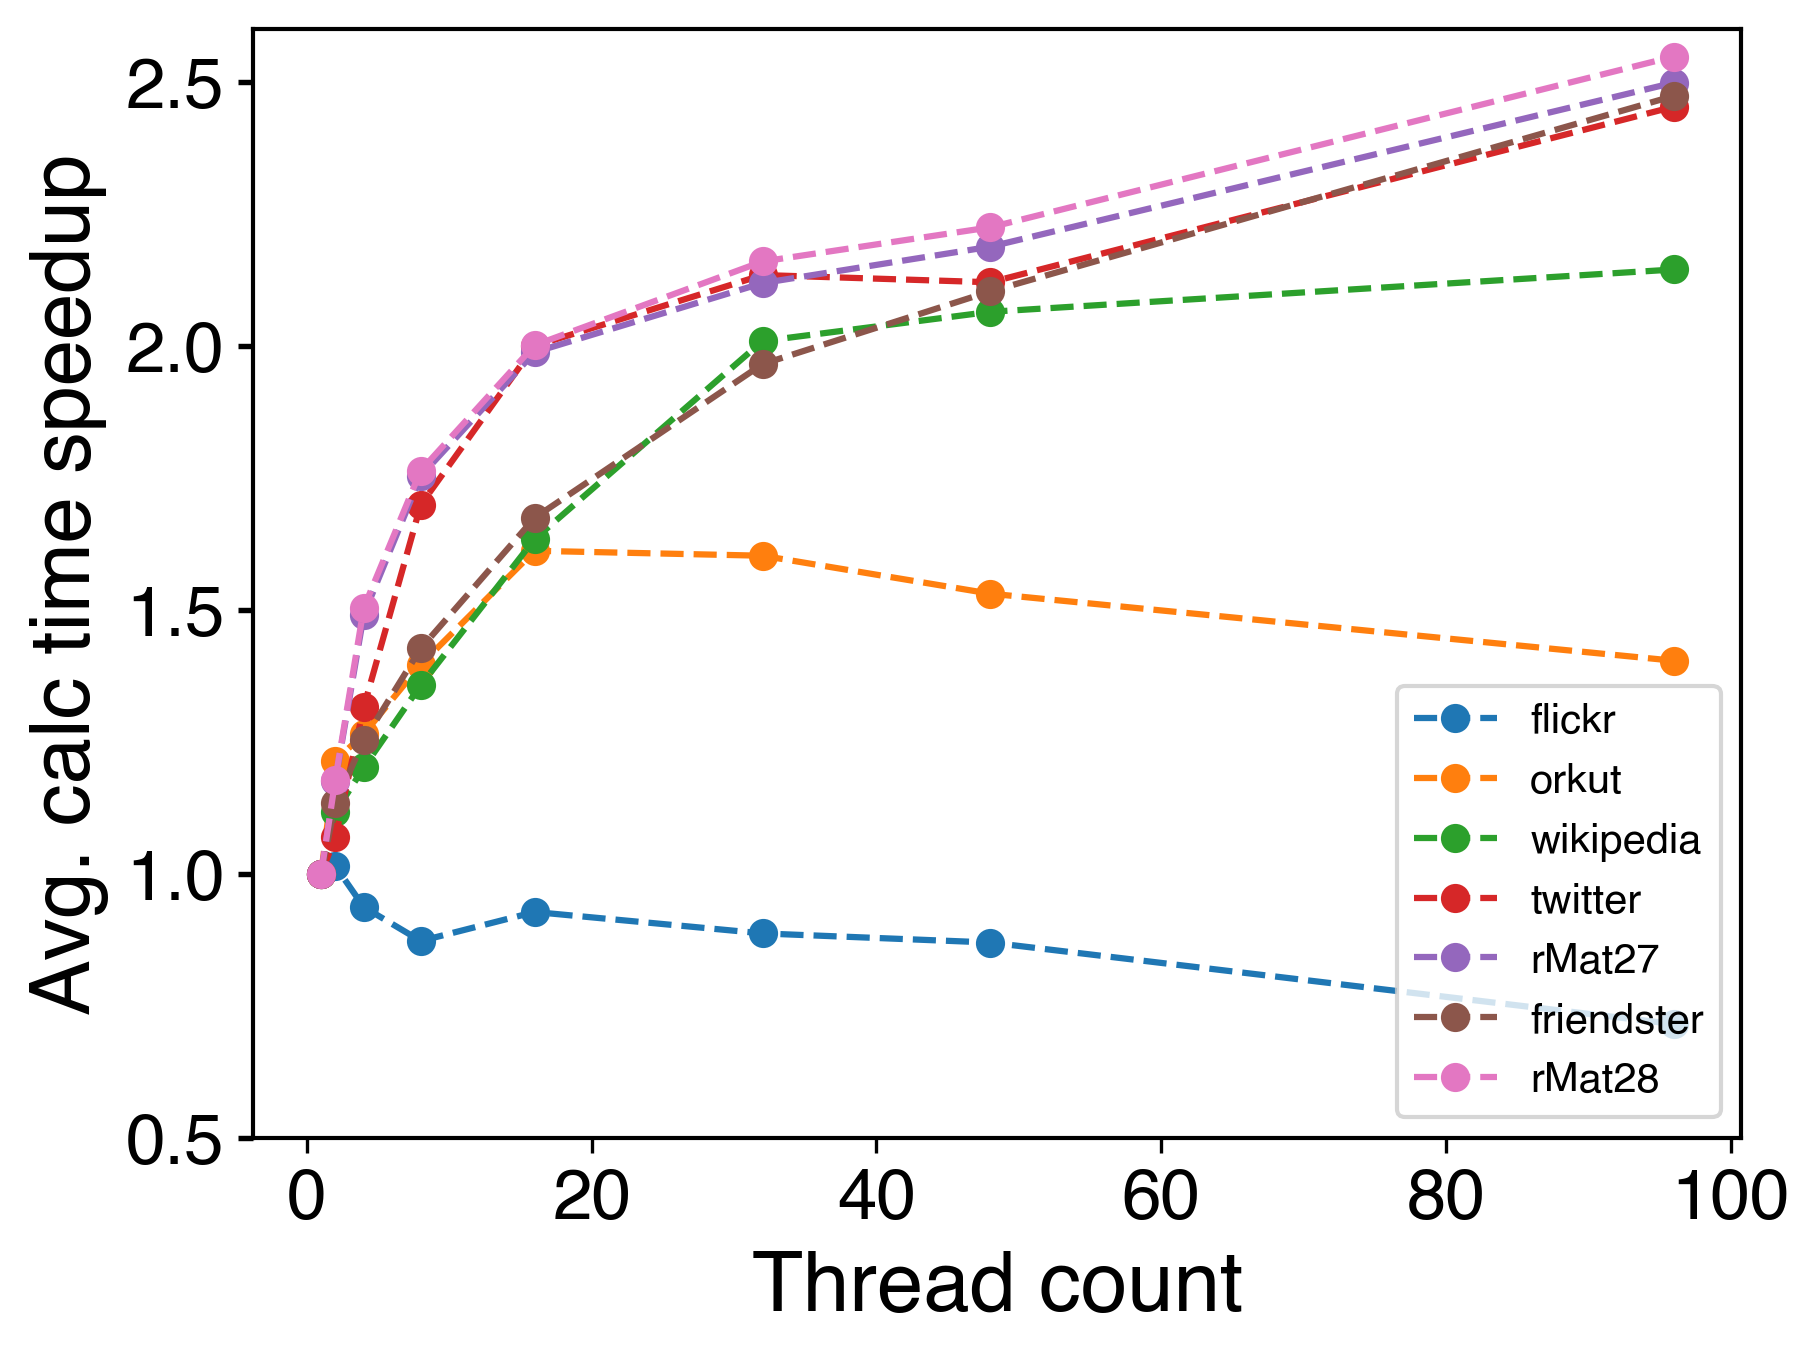
\includegraphics[width=\linewidth]{../../plots/singleNodePRPullGaloisHPThreads.png}
		\caption{PageRank Pull}
		\label{fig:galoisHPSpeedupPRPull}
	\end{subfigure}
	\begin{subfigure}{\columnwidth}
		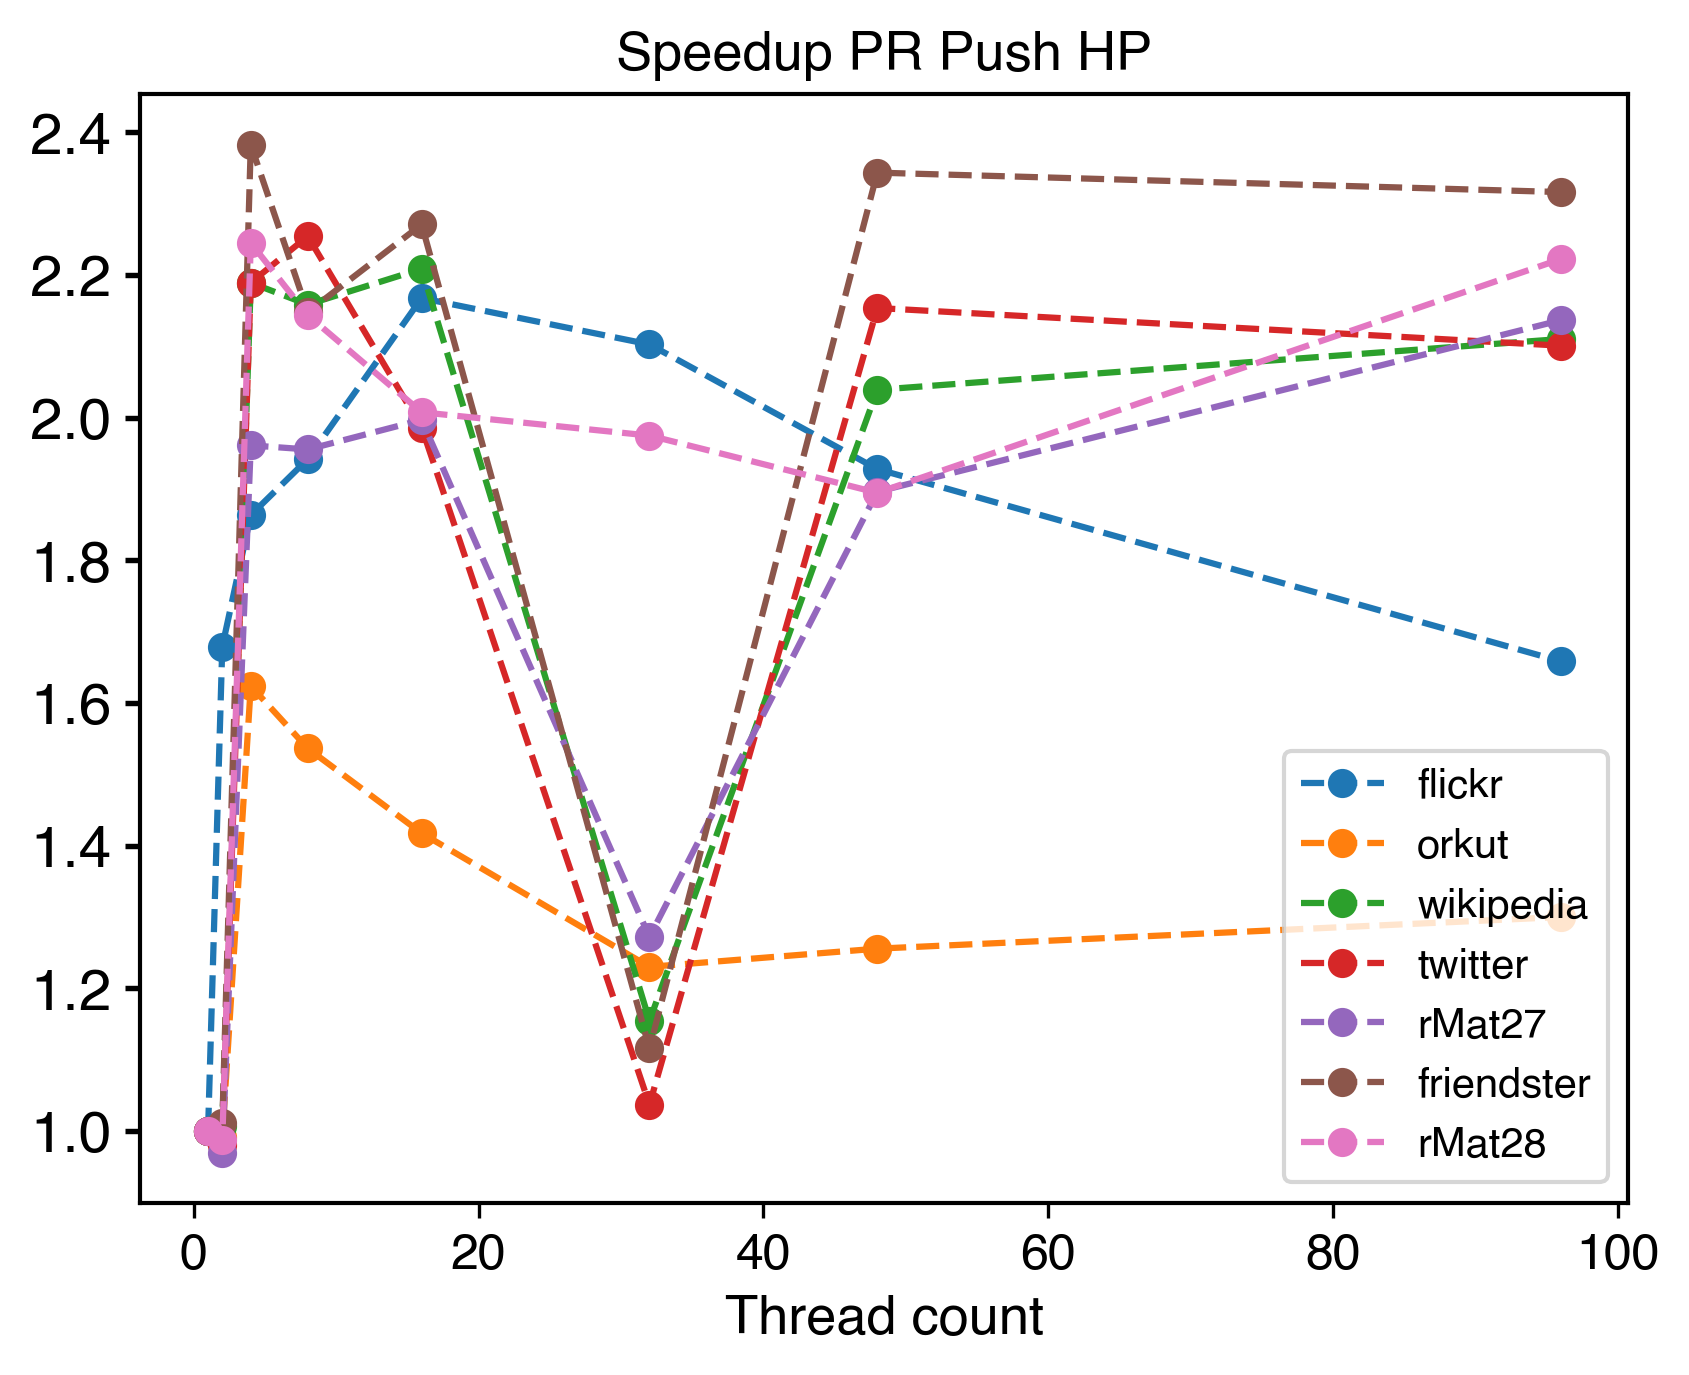
\includegraphics[width=\linewidth]{../../plots/singleNodePRPushGaloisHPThreads.png}
		\caption{PageRank Push}
		\label{fig:galoisHPSpeedupPRPush}
	\end{subfigure}
	\caption{Calculation time speedup with increasing thread count for Galois PageRank Push and Pull algorithms using Hugepages.}
\end{figure}





\section{Discussion}




\section{Conclusion}
The conclusion goes here.


\clearpage


\section*{Acknowledgment}
We are using the graph frameworks Galois~\cite{Galois}, Ligra~\cite{Ligra}, Polymer~\cite{Polymer}, Gemini~\cite{Gemini} as well as Apache Giraph~\cite{Giraph}.

Also we use Gluon~\cite{vertGalois} for the distributed Galois setups.

Gemini~\cite{Gemini}

%We would like to thank our supervisor Heiko Geppert for continued guidance and support.

\section*{Supplementary Data}\label{supplementaryData}
We have written a number of conversion tools and installation guides to help
users or developers with the use of the tested frameworks.


Our GitHub repository: \url{http://www.github.com/serengti/Forschungsprojekt}.






% Beim Hinzufügen neuer Referenzen
% 1. die beiden Zeilen nach diesem Kommentar auskommentieren.
%    (gemeint ist \bibliographystyle... und \bibliography..)
%    Dann alle cache files im Ordner löschen.
% 2. Die folgenden Commands ausführen
% pdflatex main.tex
% bibtex main
% pdflatex main.tex
%    das letzte wirft dann Fehler aber das stimmt so..
% 3. Jetzt main.bbl öffnen und den Inhalt hier drunter rein kopieren.
%    Man kann kein \input benutzen, weil main.bbl leer ist, wenn die beiden
%    Zeilen auskommentiert sind. Aber wenn sie nicht auskommentiert sind
%    kann kein PDF erzeugt werden.. Was zur Hölle denken die sich.
% 4. Die folgenden beiden Zeilen auskommentieren und pdflatex
%    ausführen wie gewohnt.


% \bibliographystyle{IEEEtran}
% \bibliography{literature}


% Alles ab hier kommt aus main.bbl

% Generated by IEEEtran.bst, version: 1.12 (2007/01/11)
% Generated by IEEEtran.bst, version: 1.12 (2007/01/11)
% Generated by IEEEtran.bst, version: 1.12 (2007/01/11)
\begin{thebibliography}{1}
\providecommand{\url}[1]{#1}
\csname url@samestyle\endcsname
\providecommand{\newblock}{\relax}
\providecommand{\bibinfo}[2]{#2}
\providecommand{\BIBentrySTDinterwordspacing}{\spaceskip=0pt\relax}
\providecommand{\BIBentryALTinterwordstretchfactor}{4}
\providecommand{\BIBentryALTinterwordspacing}{\spaceskip=\fontdimen2\font plus
\BIBentryALTinterwordstretchfactor\fontdimen3\font minus
  \fontdimen4\font\relax}
\providecommand{\BIBforeignlanguage}[2]{{%
\expandafter\ifx\csname l@#1\endcsname\relax
\typeout{** WARNING: IEEEtran.bst: No hyphenation pattern has been}%
\typeout{** loaded for the language `#1'. Using the pattern for}%
\typeout{** the default language instead.}%
\else
\language=\csname l@#1\endcsname
\fi
#2}}
\providecommand{\BIBdecl}{\relax}
\BIBdecl

\bibitem{Galois}
\BIBentryALTinterwordspacing
D.~Nguyen, A.~Lenharth, and K.~Pingali, ``A lightweight infrastructure for
  graph analytics,'' in \emph{Proceedings of the Twenty-Fourth ACM Symposium on
  Operating Systems Principles}, ser. SOSP ’13.\hskip 1em plus 0.5em minus
  0.4em\relax New York, NY, USA: Association for Computing Machinery, 2013, p.
  456–471. [Online]. Available: \url{https://doi.org/10.1145/2517349.2522739}
\BIBentrySTDinterwordspacing

\bibitem{vertGalois}
\BIBentryALTinterwordspacing
R.~Dathathri, G.~Gill, L.~Hoang, H.-V. Dang, A.~Brooks, N.~Dryden, M.~Snir, and
  K.~Pingali, ``Gluon: A communication-optimizing substrate for distributed
  heterogeneous graph analytics,'' in \emph{Proceedings of the 39th ACM SIGPLAN
  Conference on Programming Language Design and Implementation}, ser. PLDI
  2018.\hskip 1em plus 0.5em minus 0.4em\relax New York, NY, USA: Association
  for Computing Machinery, 2018, p. 752–768. [Online]. Available:
  \url{https://doi.org/10.1145/3192366.3192404}
\BIBentrySTDinterwordspacing

\bibitem{Polymer}
\BIBentryALTinterwordspacing
K.~Zhang, R.~Chen, and H.~Chen, ``Numa-aware graph-structured analytics,'' in
  \emph{Proceedings of the 20th ACM SIGPLAN Symposium on Principles and
  Practice of Parallel Programming}, ser. PPoPP 2015.\hskip 1em plus 0.5em
  minus 0.4em\relax New York, NY, USA: Association for Computing Machinery,
  2015, p. 183–193. [Online]. Available:
  \url{https://doi.org/10.1145/2688500.2688507}
\BIBentrySTDinterwordspacing

\bibitem{adjListFormat}
\BIBentryALTinterwordspacing
J.~Shun, G.~Blelloch, J.~Fineman, P.~Gibbons, A.~Kyrola, K.~Tangwonsan, and
  H.~V. Simhadri. (2020, Jun.) {Problem Based Benchmark Suite}. graphIO.html.
  [Online]. Available: \url{http://www.cs.cmu.edu/~pbbs/benchmarks/}
\BIBentrySTDinterwordspacing

\bibitem{Ligra}
\BIBentryALTinterwordspacing
J.~Shun and G.~E. Blelloch, ``Ligra: A lightweight graph processing framework
  for shared memory,'' in \emph{Proceedings of the 18th ACM SIGPLAN Symposium
  on Principles and Practice of Parallel Programming}, ser. PPoPP ’13.\hskip
  1em plus 0.5em minus 0.4em\relax New York, NY, USA: Association for Computing
  Machinery, 2013, p. 135–146. [Online]. Available:
  \url{https://doi.org/10.1145/2442516.2442530}
\BIBentrySTDinterwordspacing

\bibitem{Gemini}
\BIBentryALTinterwordspacing
X.~Zhu, W.~Chen, W.~Zheng, and X.~Ma, ``Gemini: A computation-centric
  distributed graph processing system,'' in \emph{12th {USENIX} Symposium on
  Operating Systems Design and Implementation ({OSDI} 16)}.\hskip 1em plus
  0.5em minus 0.4em\relax Savannah, GA: {USENIX} Association, Nov. 2016, pp.
  301--316. [Online]. Available:
  \url{https://www.usenix.org/conference/osdi16/technical-sessions/presentation/zhu}
\BIBentrySTDinterwordspacing

\bibitem{Giraph}
\BIBentryALTinterwordspacing
A.~S. Foundation. (2020, Jun.) {Apache Giraph}. [Online]. Available:
  \url{https://giraph.apache.org}
\BIBentrySTDinterwordspacing

\bibitem{konect}
J.~Kunegis, ``Konect: the koblenz network collection,'' 05 2013, pp.
  1343--1350.

\end{thebibliography}


% Alles bis hier kommt aus main.bbl



\end{document}
